\documentclass[11pt]{report}
%% Useful packages
\usepackage[utf8]{inputenc}
\usepackage[a4paper,margin=20mm]{geometry}
\usepackage{crop,graphicx,amsmath,array,color,amssymb,fancyhdr,lineno,float,booktabs}
\usepackage{flushend,stfloats,amsthm,chngpage,times,,lipsum,lastpage,parskip,adjustbox} 
\usepackage{calc,listings,color,wrapfig,tabularx,longtable,multirow,enumitem,commath,siunitx}
\usepackage[table,xcdraw]{xcolor}
\usepackage[]{quoting}
%\usepackage[numbers]{natbib}
%\usepackage[subtle]{savetrees}
\usepackage[
  nottoc
  %notlot
  %notlof
]{tocbibind}

\usepackage{hyperref}
\hypersetup{
    colorlinks=true,
    linkcolor=black,
    filecolor=teal,      
    urlcolor=teal,
    citecolor=teal,
    pdftitle={MECH0071 Topic Notes},
    pdfauthor={HD},
    pdfpagemode=FullScreen,
}

\renewcommand\bibname{References}
\usepackage{lineno}
%%%%%%%%%%%%   Header and Footer  %%%%%%%%%%%%%
\pagestyle{fancy}
\fancypagestyle{plain}{%
  \renewcommand{\headrulewidth}{0pt}%
  \fancyhf{}%
  \addtolength{\topmargin}{-2pt}
}

\title{%
  Topic Notes}
\author{HD
}

\begin{document}
\begin{titlepage}

  \newcommand{\HRule}{\rule{\linewidth}{0.5mm}} % Defines a new command for the horizontal lines, change thickness here

  %----------------------------------------------------------------------------------------
  %	LOGO SECTION
  %----------------------------------------------------------------------------------------
  \center
  
\includegraphics[width=5cm]{Title/UCL.png}\\[1cm] % Include a department/university logo - this will require the graphicx package

  %----------------------------------------------------------------------------------------

  \center % Center everything on the page

  %----------------------------------------------------------------------------------------
  %	HEADING SECTIONS
  %----------------------------------------------------------------------------------------

  \textsc{\LARGE University College London }\\[1.5cm] % Name of your university/college
  \textsc{\Large MEng Mechanical Engineering  }\\[0.5cm] % Major heading such as course name
  \textsc{\large MECH0071 Electrical Power Systems and Electrical Propulsion }\\[1.5cm] % Minor heading such as course title

  %----------------------------------------------------------------------------------------
  %	TITLE SECTION
  %----------------------------------------------------------------------------------------
  \makeatletter
  { \huge \textsc \@title}\\[1.5cm] % Title of your document


  %----------------------------------------------------------------------------------------
  %	AUTHOR SECTION
  %----------------------------------------------------------------------------------------

  \begin{minipage}{0.4\textwidth}
    \begin{flushleft} \large
      \emph{Author:}\\
      \@author % Your name
      \\[1.2em]
      %\emph{ID No:}\\
      %0101010 \\[1.2em]
    \end{flushleft}
  \end{minipage}
  ~
  \begin{minipage}{0.4\textwidth}
    \begin{flushright} \large
      \emph{Module coordinator:} \\
      Prof. Richard Bucknall \\[1.2em] % Supervisor's Name
      %\emph{Module teaching team:} \\
      %Dr. Tim Hillel\\ % second marker's name
      %Mr. Umut Lagap
    \end{flushright}
  \end{minipage}\\[2cm]
  \makeatother

  % If you don't want a supervisor, uncomment the two lines below and remove the section above
  %\Large \emph{Author:}\\
  %John \textsc{Smith}\\[3cm] % Your name

  %----------------------------------------------------------------------------------------
  %	DATE SECTION
  %----------------------------------------------------------------------------------------

  {\large \today}\\[2cm] % Date, change the \today to a set date if you want to be precise

  \vfill % Fill the rest of the page with whitespace

\end{titlepage}

\fancyhf{}
\fancyhead[L]{MECH0071}
\fancyfoot[L]{HD}
\fancyfoot[R]{ \bf\thepage\ \rm }%

\newpage
\tableofcontents
\newpage
\listoffigures
\listoftables
\newpage

\chapter{The Electrical Line Diagram}
\section{Overview of electrical power systems}
\subsection{Basic electrical power system}
Most electrical power systems contain:
\begin{itemize}
  \item Generators to produce electrical energy (often coming from another store of energy e.g. chemical - oil, gas, coal)
  \item A means to transmit and distribute the electrical energy
  \item Loads that use the electrical energy for some purpose
\end{itemize}
\subsection{What is an electrical power system?}
\textbf{An electric power system} is a network or grid of electrical components that supply, transfer and use electric energy. Electrical power systems can be a:
\begin{itemize}
  \item Large grids covering a wide area e.g. a continent
  \item Medium grid covering a large area e.g. a country
  \item Small network covering a small area e.g. a ship
\end{itemize}
\section{Components of electrical power systems}
\subsection{Sources of electrical power include}
Generators (rotating types AC and DC):
\begin{itemize}
  \item Large AC generators e.g. \SI{25}{\kilo\volt} three-phase voltages
  \item Medium AC generators e.g. \SI{440}{\volt} three-phase voltages
  \item Small AC generators e.g. e.g. single-phase \SI{220}{\volt} voltages
\end{itemize}
Fuel cells:
\begin{itemize}
  \item DC output voltage (typically \SI{720}{\volt} DC)
\end{itemize}
Batteries (electro-chemical):
\begin{itemize}
  \item DC output voltage (usually multiples of \SI{12}{\volt})
\end{itemize}
Photo-voltaic (solar) cells:
\begin{itemize}
  \item DC output currents (usually mA/cell)
\end{itemize}
\subsection{Sources of DC electrical power \dots}
A fuel cell in a car. Photovoltaics used in a solar farm. Battery energy store. DC systems are increasing in their popularity due to wider use of batteries, solar cells and fuel cells in grids and electrical propulsion.
\subsection{Generators \dots single and multiphase AC}
AC generators:
\begin{itemize}
  \item Large AC generators e.g. \SI{25}{\kilo\volt} 3 phase
  \item Medium AC generators e.g. \SI{11}{\kilo\volt} or \SI{440}{\volt} 3 phase
  \item Small generators e.g. \SI{220}{\volt} single-phase voltage
\end{itemize}
\subsection{Transmission systems}
HVAC often three-wire and three-phase e.g. \SI{440}{\kilo\volt}, \SI{275}{\kilo\volt} and \SI{132}{\kilo\volt}.

HVDC often two-wire and bipolar e.g. +/- \SI{330}{\kilo\volt}.
\subsection{Distribution systems}
AC distribution:
\begin{itemize}
  \item \SI{11}{\kilo\volt}, \SI{440}{\volt} three-phase
  \item \SI{25}{\kilo\volt} single-phase (rail)
  \item \SI{240}{\volt} single-phase
\end{itemize}
DC distribution:
\begin{itemize}
  \item \SI{750}{\volt} (rail)
  \item \SI{110}{\volt} (emergency lighting)
\end{itemize}
\subsection{Loads}
Three-phase loads:
\begin{itemize}
  \item Induction motors to drive pumps, fans and compressors
  \item Propulsion drives
\end{itemize}
Single-phase loads:
\begin{itemize}
  \item Lighting
  \item Heating
  \item Appliances e.g. domestic, electronics, small pumps
\end{itemize}
DC loads:
\begin{itemize}
  \item DC motors
  \item Lighting and heating
  \item Battery charging
\end{itemize}
\section{Representation by the electrical line diagram}
\subsection{Electrical system representation}
Electrical systems are commonly represented as one of the following:
\begin{itemize}
  \item Pictorial diagram
  \item Block diagram
  \item Wiring diagram
  \item Single line diagram
  \item Riser diagram
  \item Electrical floor plan
  \item Layout diagram
\end{itemize}
Of these the most useful to the \textit{electrical power engineer} is the \textbf{Single line diagram.}
\begin{figure}[H]
  \centering
  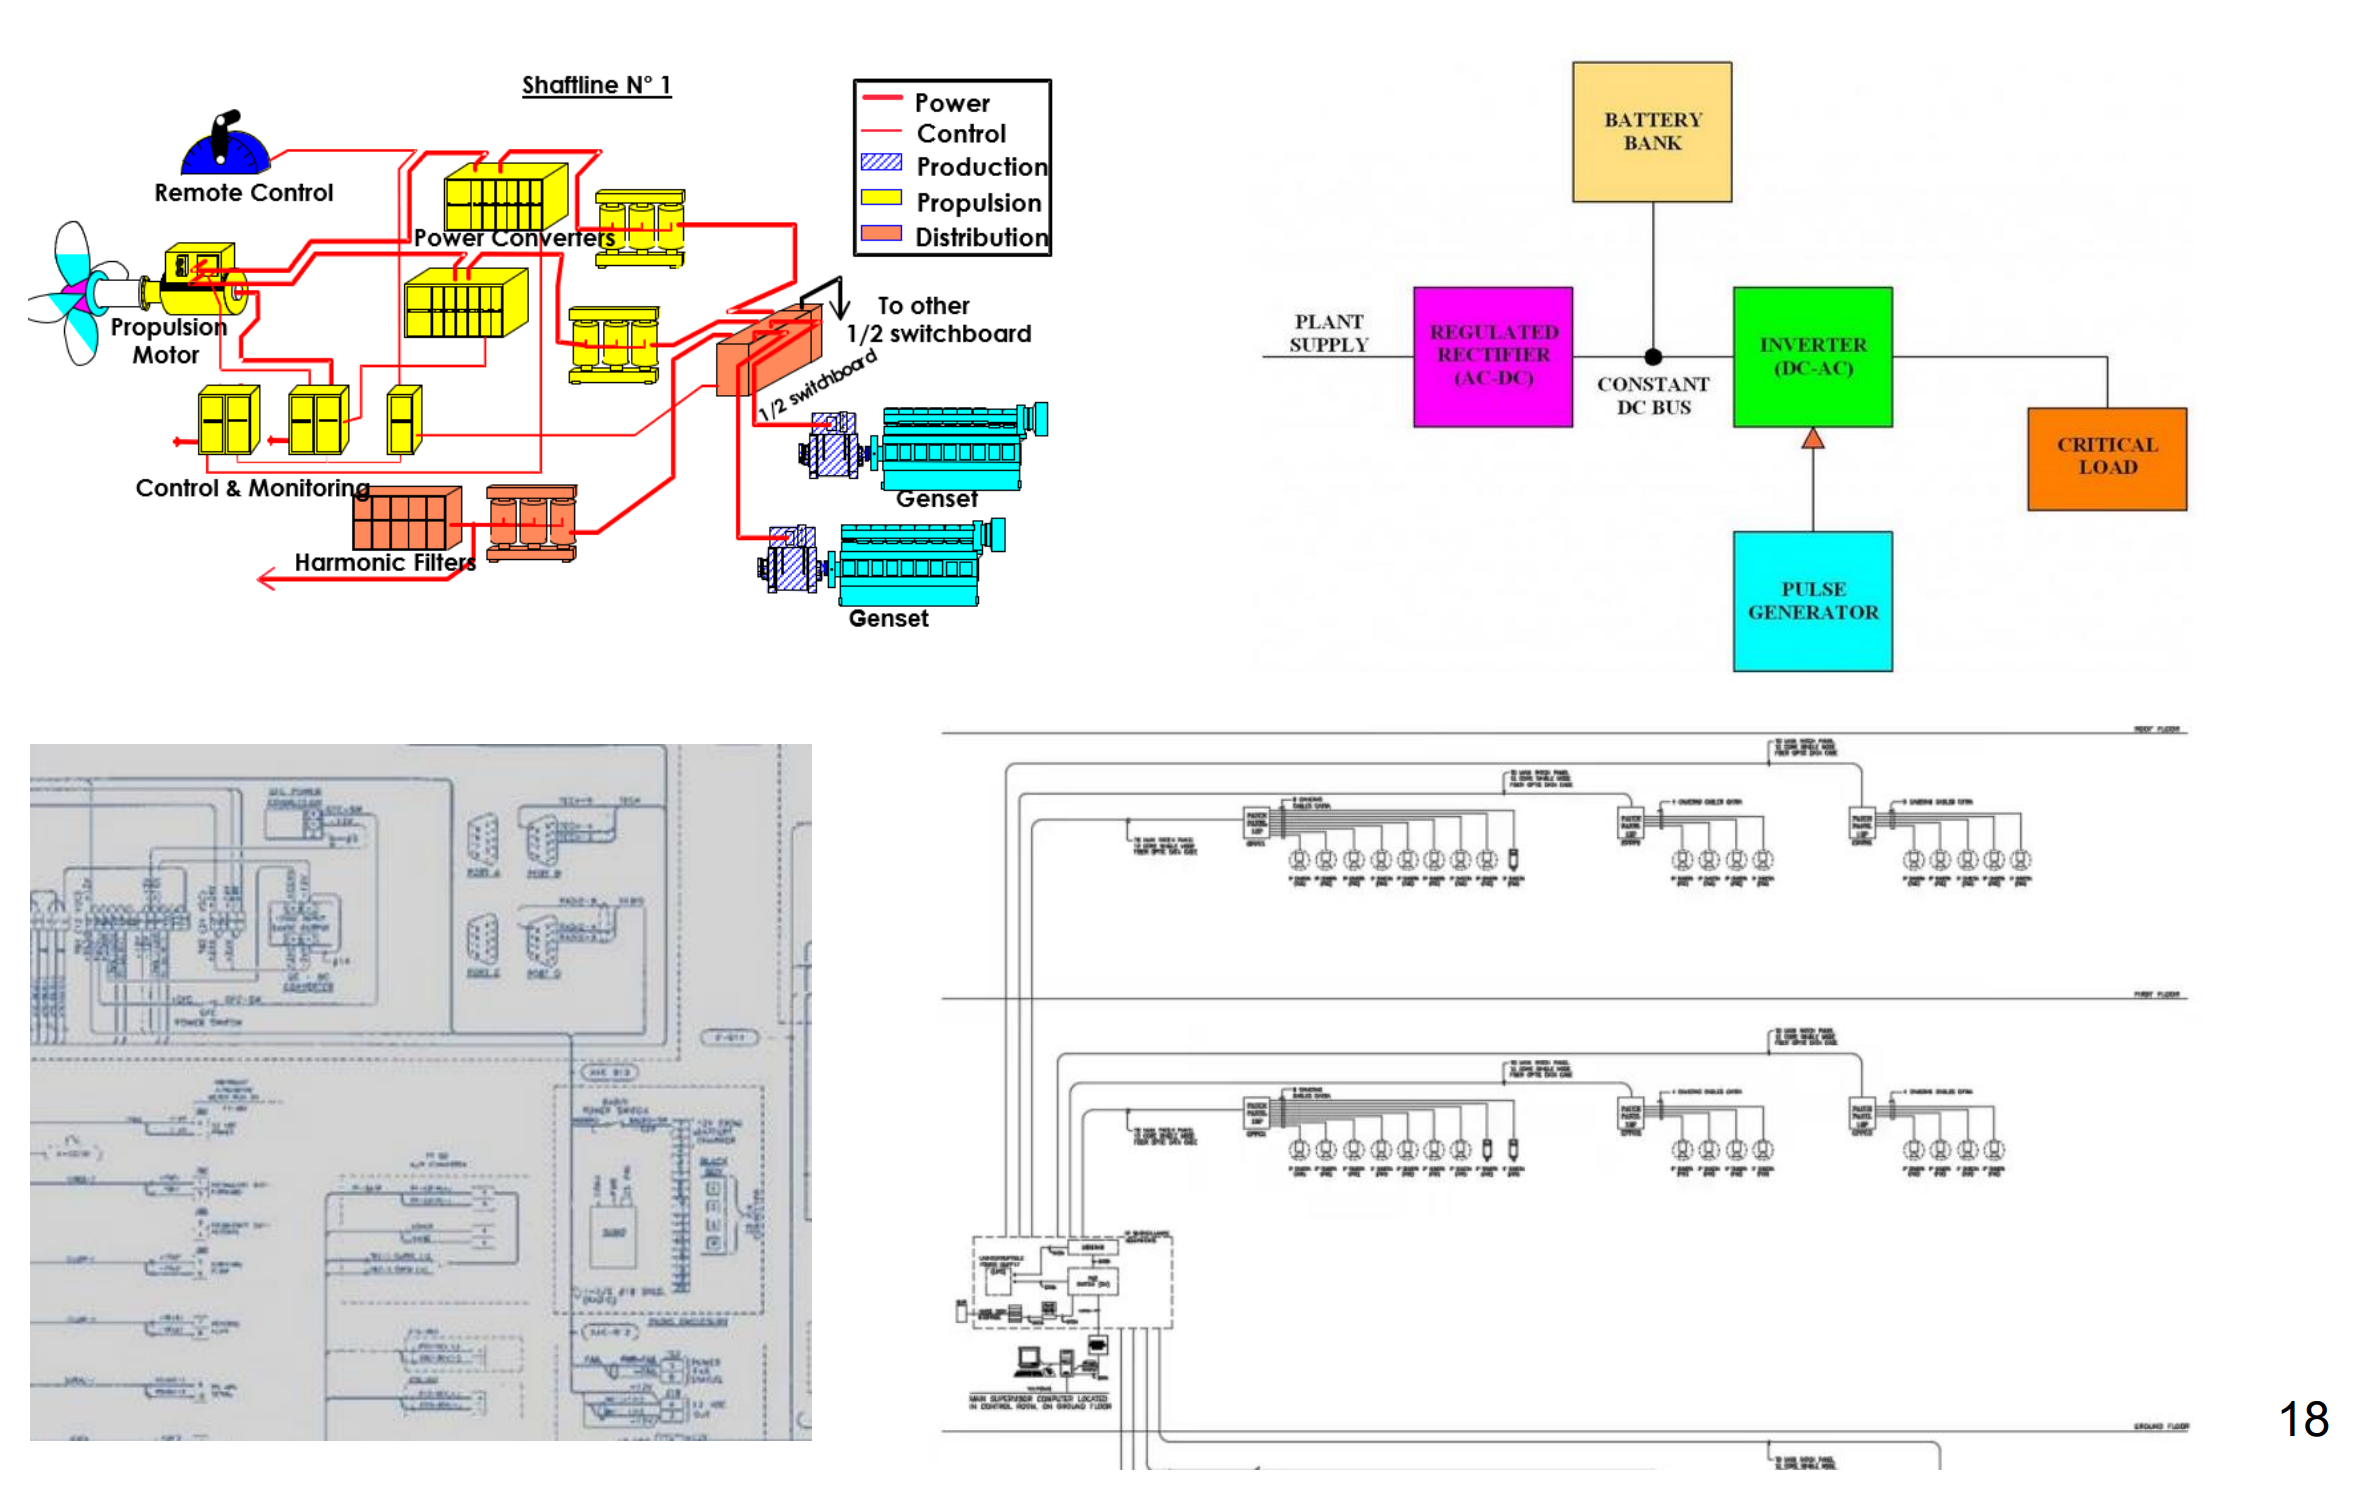
\includegraphics[width = \textwidth]{./img/figure1.png}
  \caption{Some types of electrical system representation.}
\end{figure}
\begin{figure}[H]
  \centering
  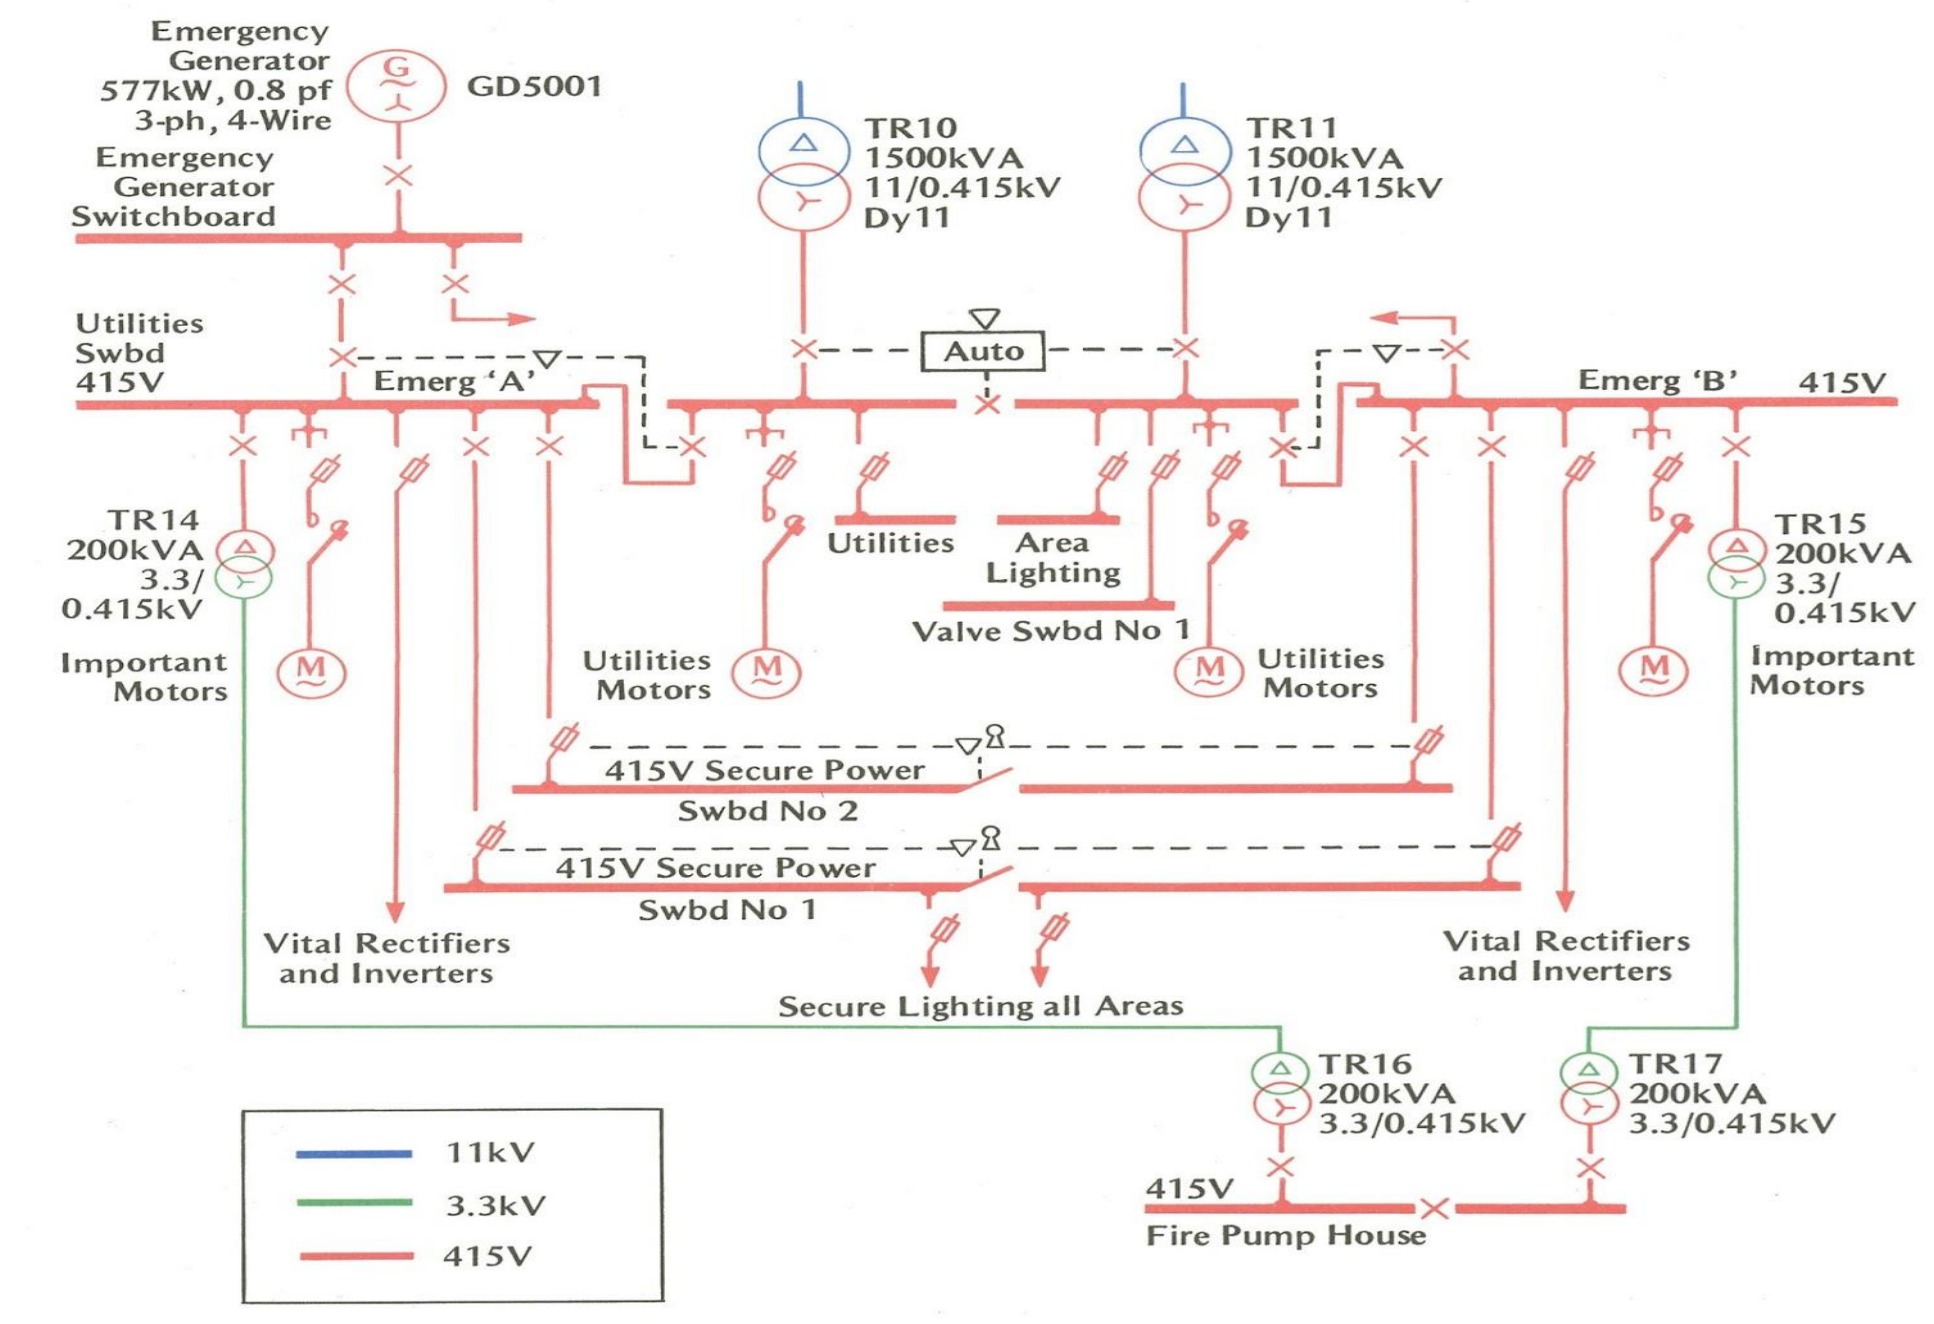
\includegraphics[width = \textwidth]{./img/figure2.png}
  \caption{Example of a `Single Line diagram'.}
\end{figure}
\subsection{Questions for you?}
\begin{enumerate}
  \item The number of separate switchboards shown? 14 (each thick line is a separate switchboard)
  \item Maximum current that will flow through the supply transformers? $I = \dfrac{\si{\kilo\volt\ampere}}{\si{\kilo\volt} \times \sqrt{3}}$, (root 3 due to 3-phase)
  \item How many different electrical sources supply the fire pump house? All three supplies can be connected to the fire pump house.
        \begin{figure}[H]
          \centering
          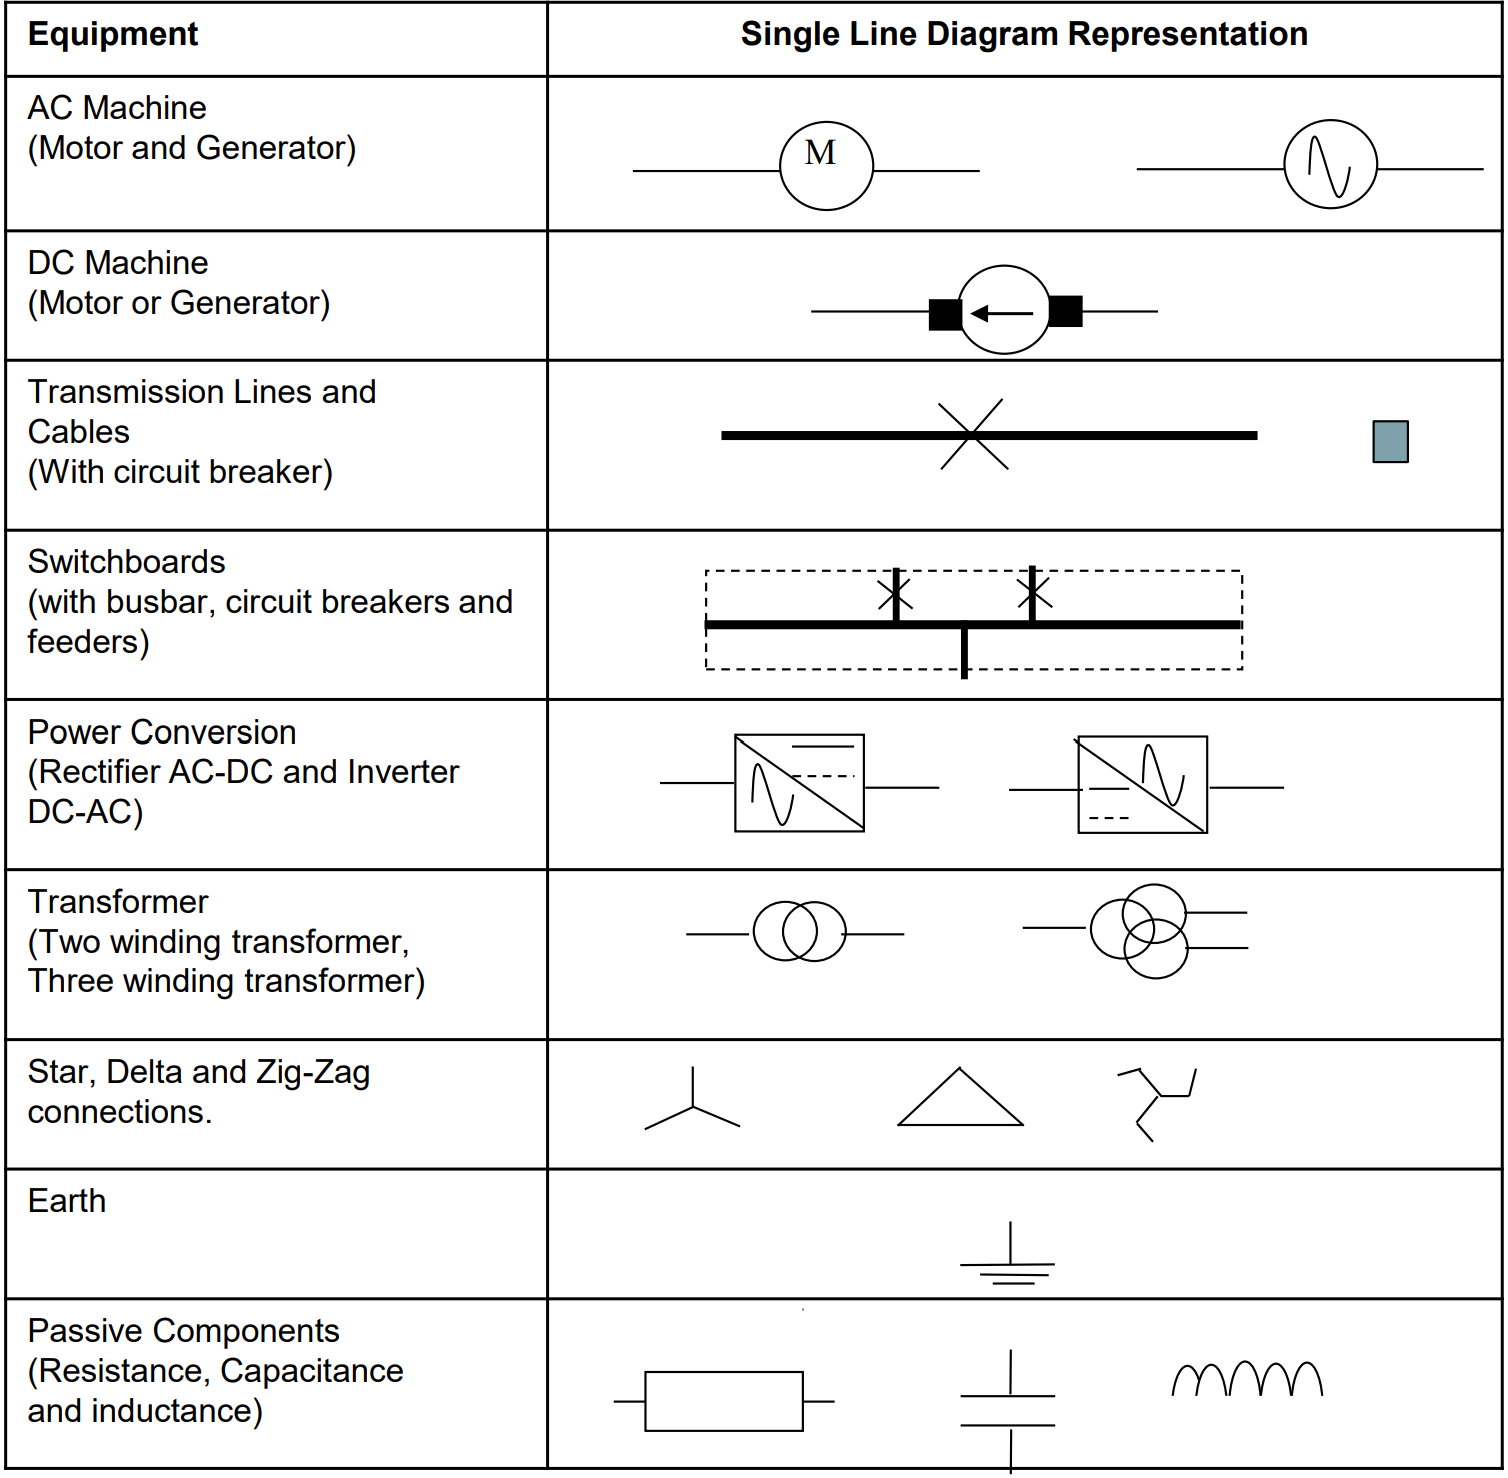
\includegraphics[width = \textwidth]{./img/figure3.png}
          \caption{Symbols.}
        \end{figure}
\end{enumerate}
\subsection{The `Single Line Diagram' (SLD)}
The `Single Line Diagram' (also known as the `One Line Diagram') represents an electrical power system using single lines regardless of number of cables being used. It can be used to represent:
\begin{itemize}
  \item Any type of electrical power system: DC, single-phase, three-phase or a mixed voltage electrical system.
  \item The interconnections between different electrical equipment including generators, switchboards, electrical distribution centres and loads.
  \item The types of electrical equipment and their main characteristics e.g. ratings of equipment such as voltage, power, power factor, and impedance.
  \item Emergency features such as reversionary modes, cross-connections and emergency generators. Sometimes these can be represented as single `dotted line' connections rather than the usual solid single line.
  \item Other details such as `earthing arrangements, arrangements of star/delta connections in three-phase systems and any autonomous operating systems such as circuit breakers.
\end{itemize}
\begin{figure}[H]
  \centering
  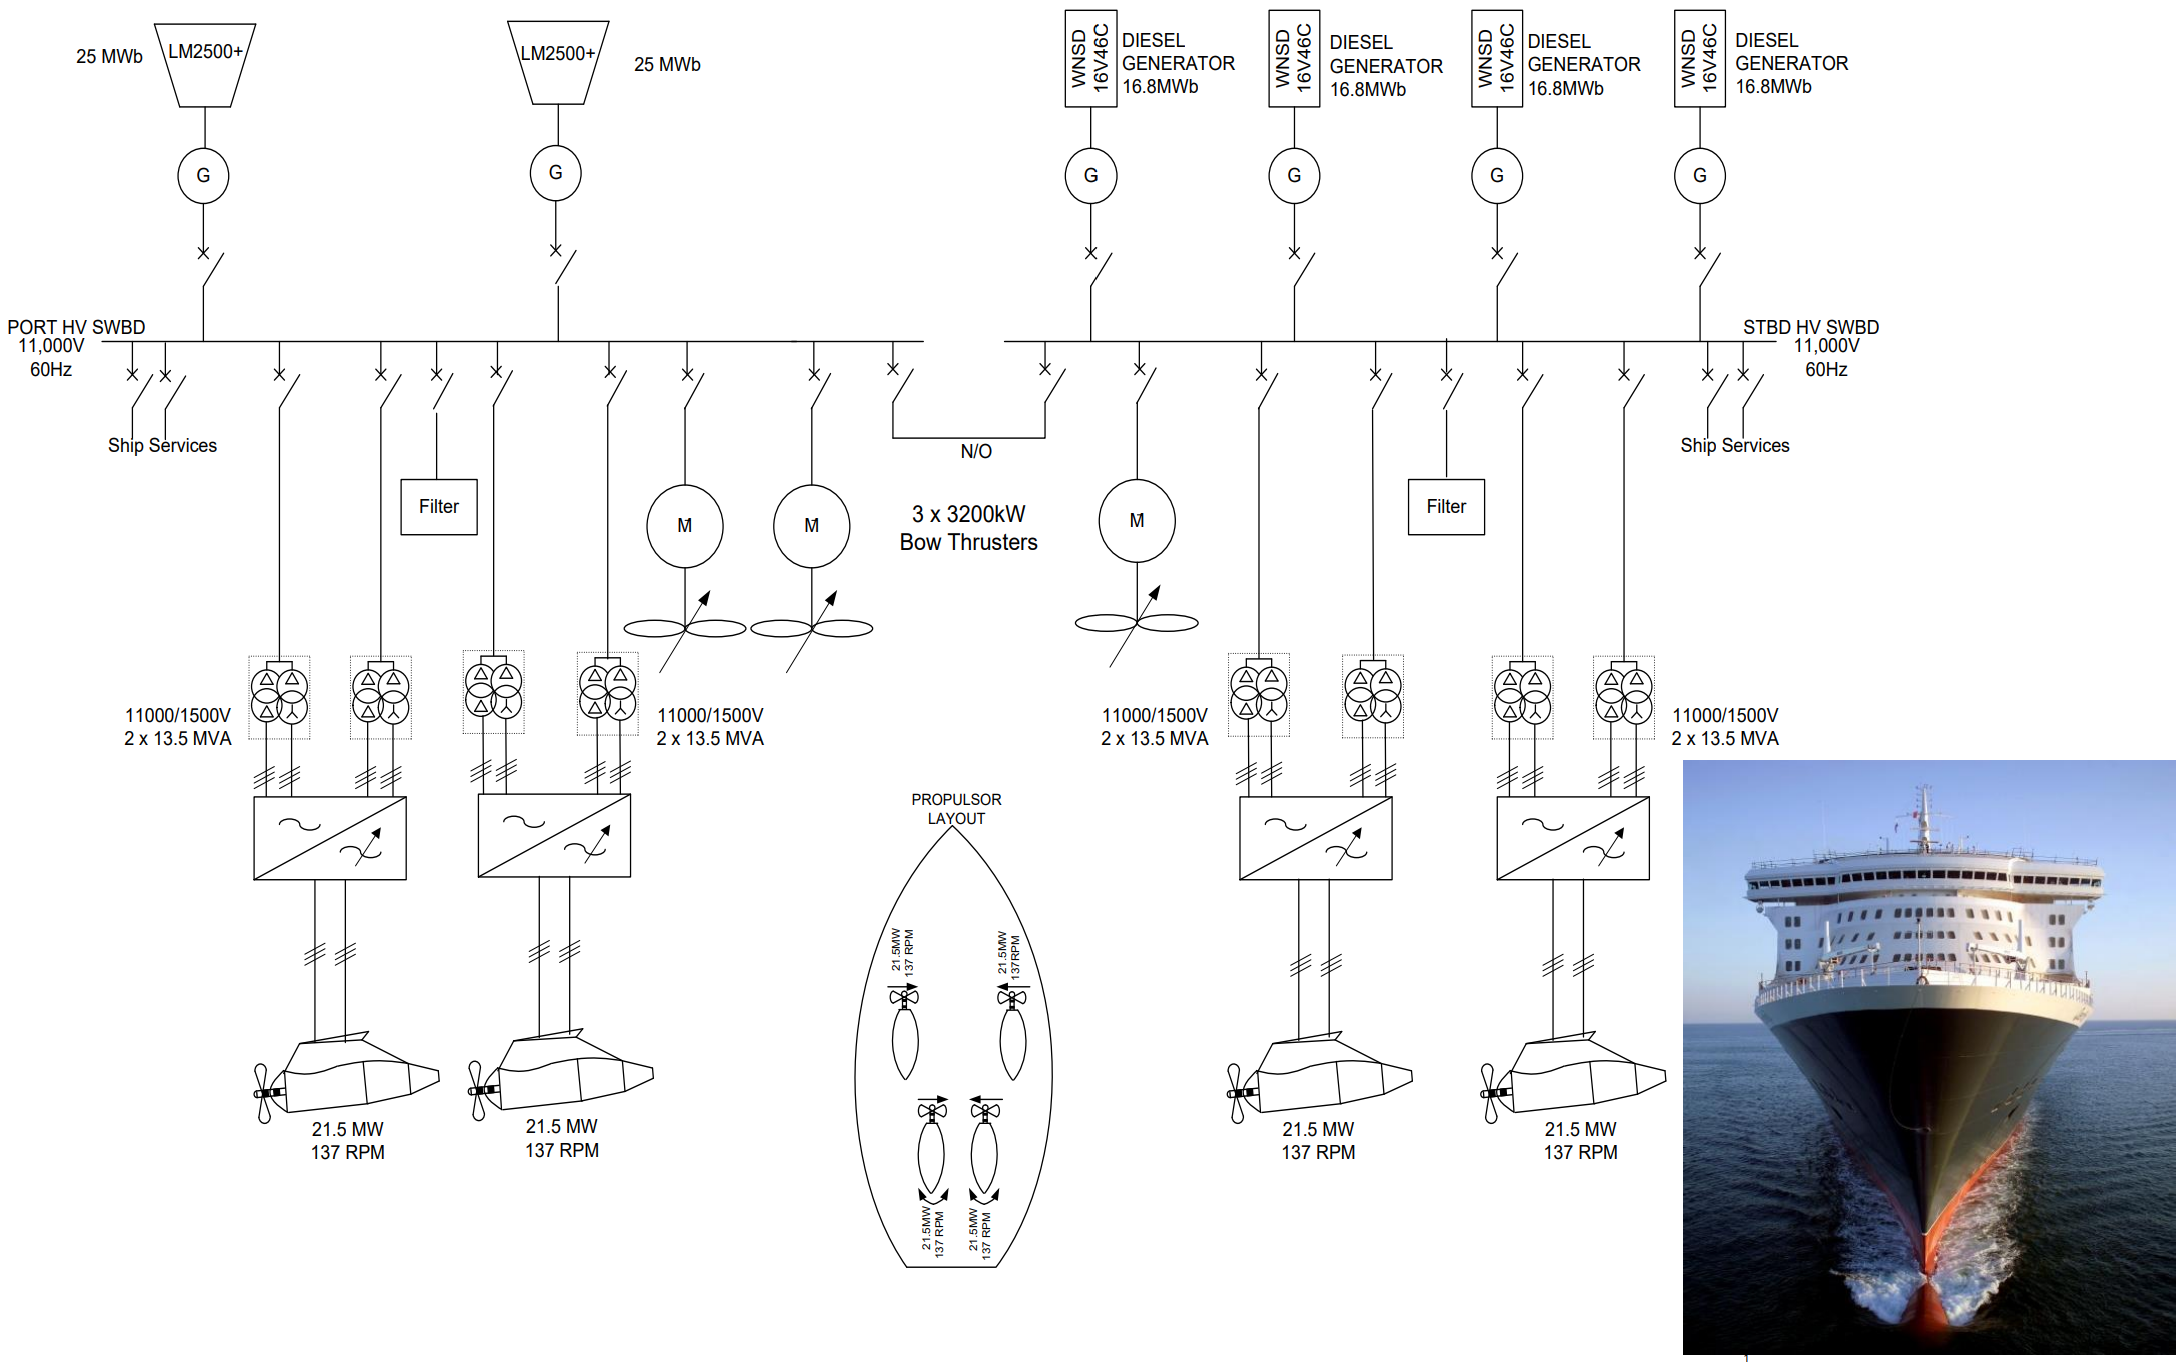
\includegraphics[width = \textwidth]{./img/figure4.png}
  \caption{Marine SLD.}
\end{figure}
\begin{figure}[H]
  \centering
  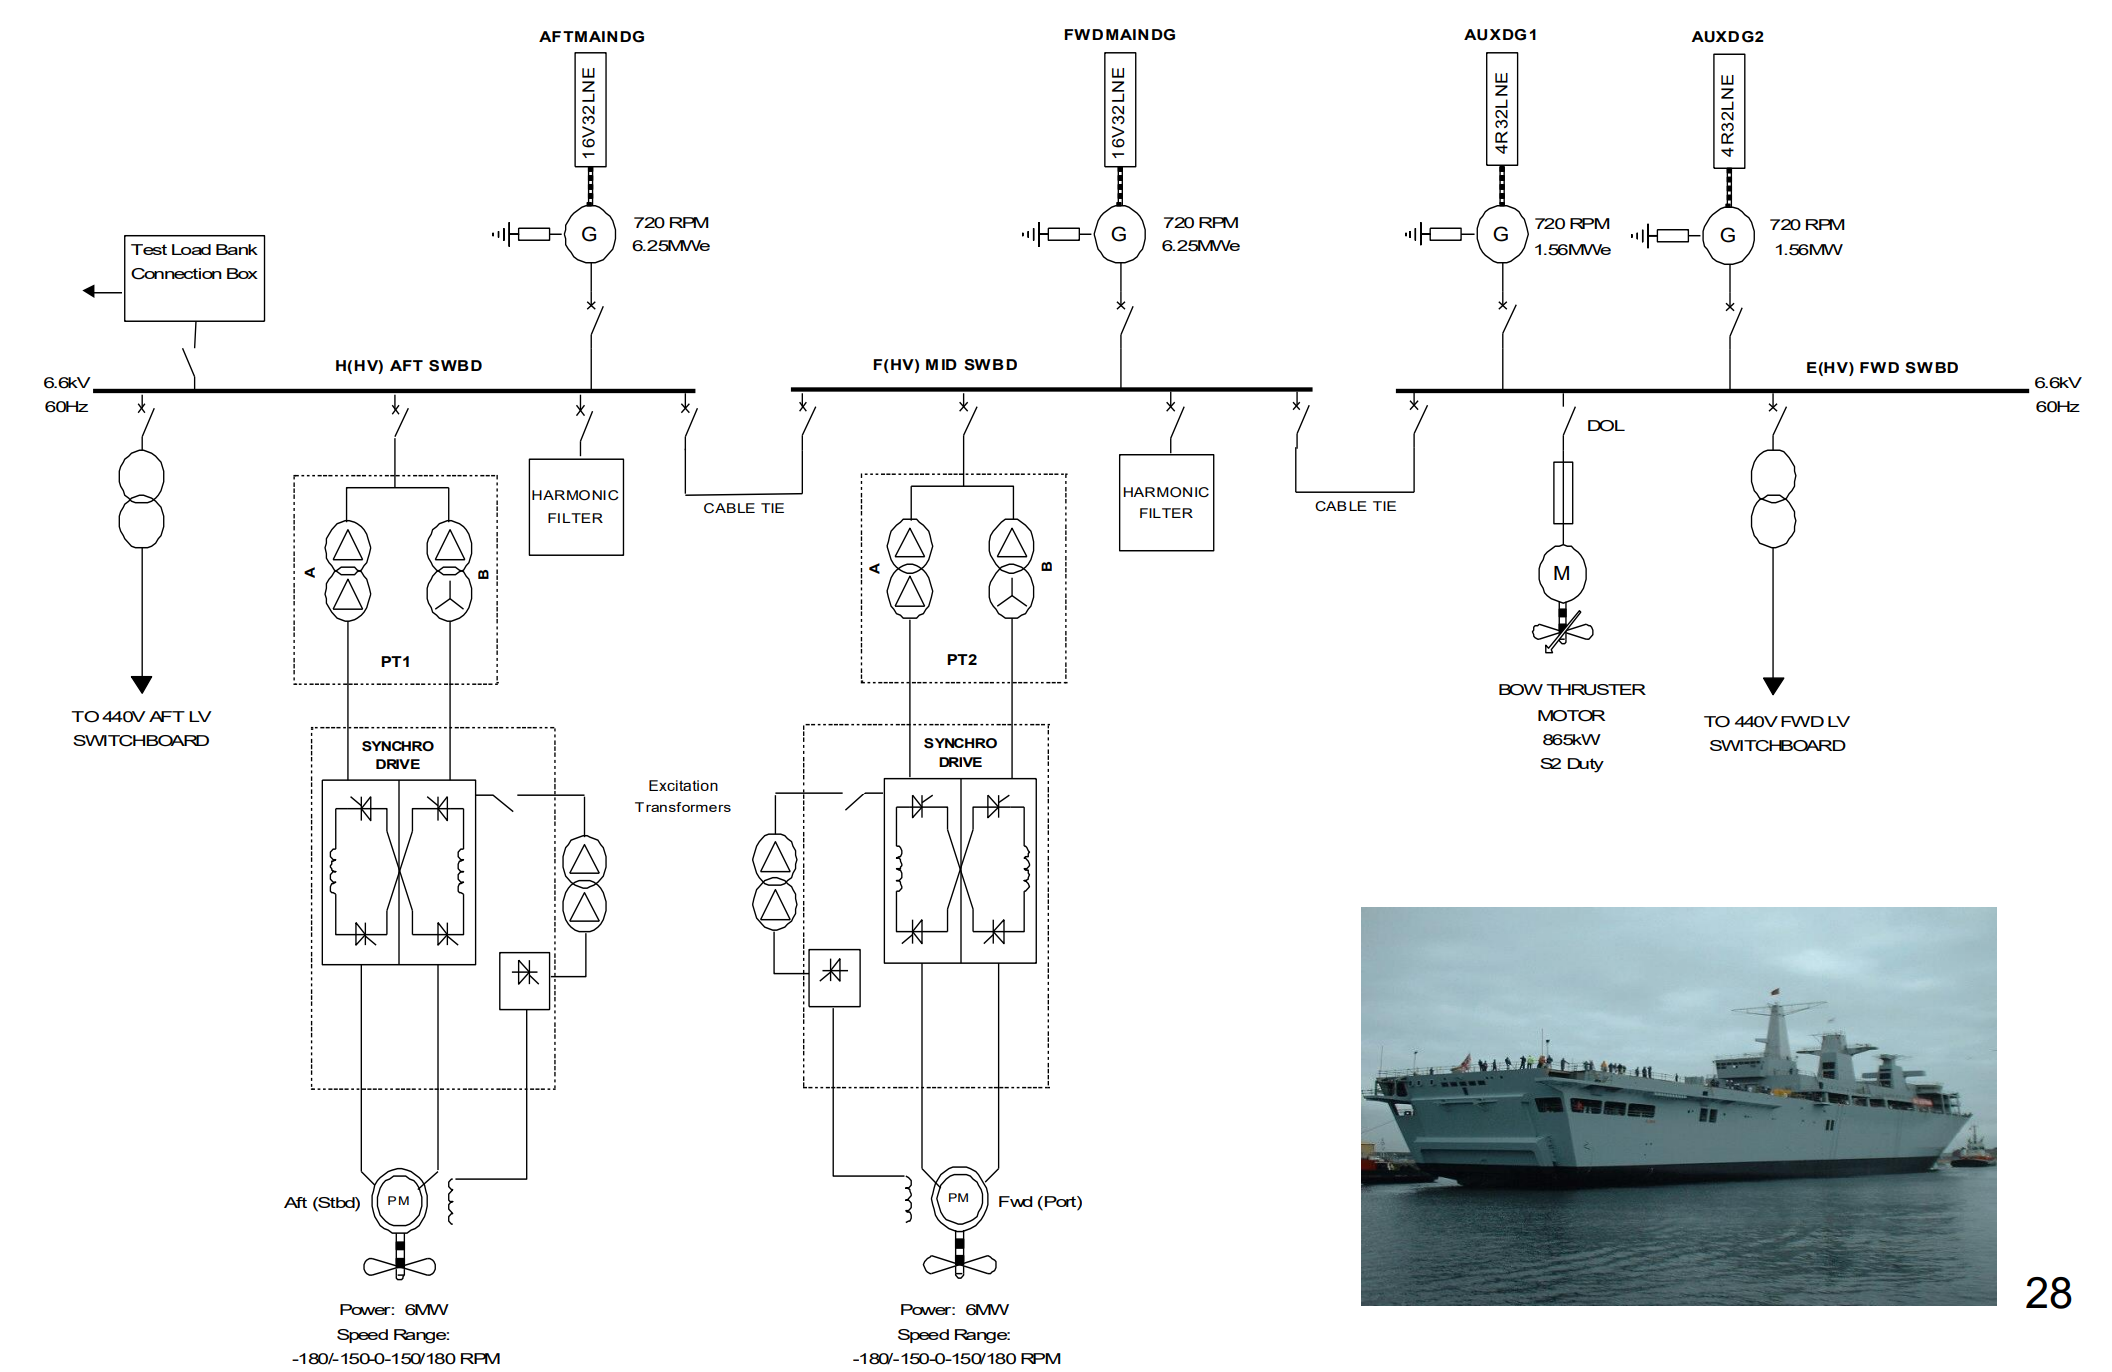
\includegraphics[width = \textwidth]{./img/figure5.png}
  \caption{Naval SLD.}
\end{figure}
\subsection{Some common features of SLDs}
\begin{itemize}
  \item Supplies (shore supplies, generators, incoming supply) are located at the top of the diagram
  \item The loads (motors, lighting, etc.) are located towards the bottom of the diagram.
  \item Switchboards are shown as thicker lines with interlocking switchgear being shown using dotted lines.
  \item Interconnections between equipment is a single-line representation regardless of number of phase (unless there is a good reason not to do so).
  \item Voltage, Frequency, Power, PF, revolutions, etc. are provided.
\end{itemize}
\subsection{Limitations of the electrical line diagram}
\begin{itemize}
  \item The `Single Line Electrical Diagram' is a very useful means of showing how electrical equipment is connected into a system using single lines (representing a three-phase system or some other electrical power system).
  \item It has very limited use when undertaking analysis. It is not an electrical circuit. To undertake analysis of electrical power systems then it is necessary to change the `Single Line Electrical Diagram' into an `Impedance Diagram'.
\end{itemize}














\chapter{Developing Impedance Diagram}
\section{Three Phase Power}
\subsection{Three-phase alternating voltages}
A three-phase synchronous generator consists of a rotor and a stator.
\begin{itemize}
	\item Adjusting excitation current on the rotating field will change the magnitude of the three AC phase emfs generated in the stator.
	\item Changing the rotational speed changes the frequency of the AC emfs
	\item The three phases generated are \SI{120}{\degree} displaced due to special arrangement
\end{itemize}
\subsection{Three-phase emfs (or terminal voltages) can be expressed mathematically}
\begin{align}
	v_a\left( t\right) & = V_m \sin\left( \omega t\right)                  \\
	v_b\left( t\right) & = V_m \sin\left( \omega t - \frac{2\pi}{3}\right) \\
	v_c\left( t\right) & = V_m \sin\left( \omega t - \frac{4\pi}{3}\right)
\end{align}
$V_m$ is the peak (maximum) voltage, $\omega$ is the angular frequency, $t$ is time. The phase displacement between the three-phase waveforms is \SI{120}{\degree} or $\frac{2\pi}{3}$ radians. $v_a$, $v_b$ and $v_c$ are the three phase voltages.
\subsection{Three-phase, six-wire connection}
The are different arrangements for distributing three-phase electrical power. The three phases can be independent of each other as seen below and treated as three separate circuits. This is known as the \textit{three-phase, six-wire system}.
\begin{figure}[H]
	\centering
	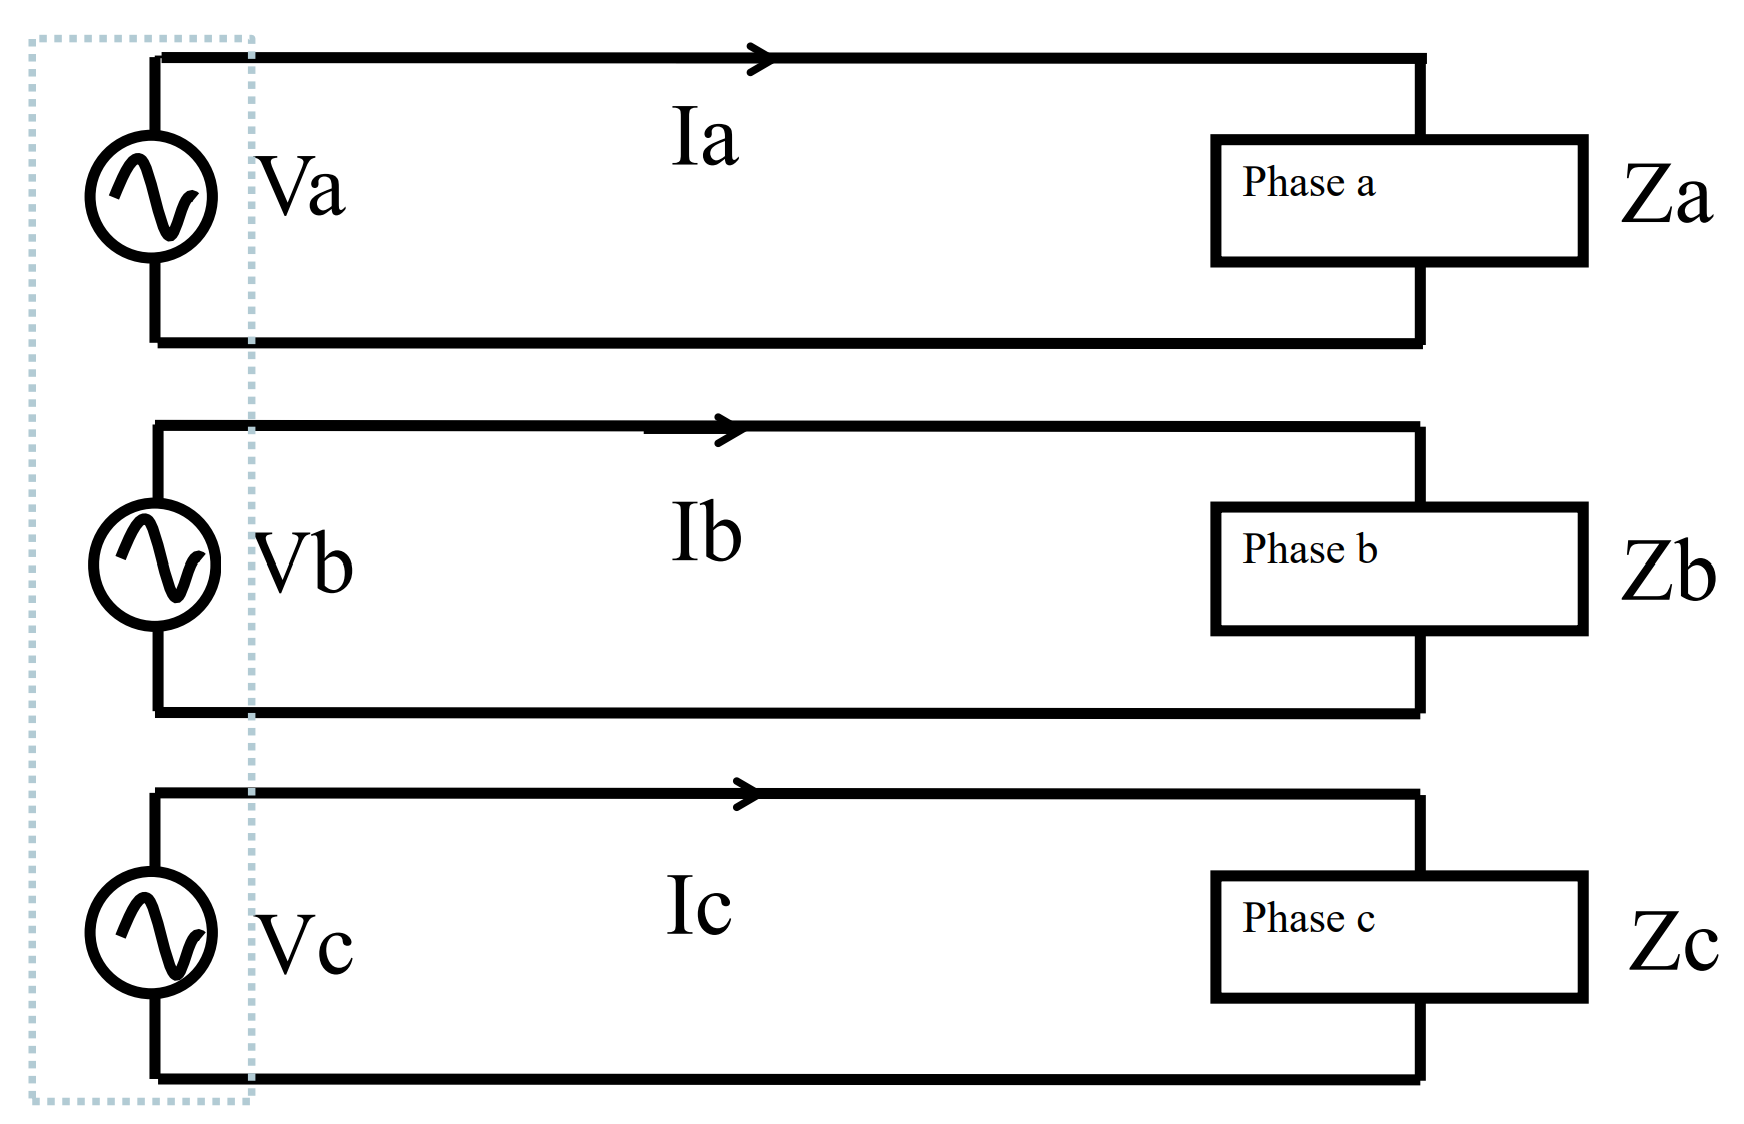
\includegraphics[width = 0.9\textwidth]{./img/figure6.png}
	\caption{Three-phase, six-wire system.}
\end{figure}
\subsection{Three-phase current}
\begin{quoting}
	The currents flow in a three-phase circuit when there is a three-phase load. We will initially assume that the three-phase load is balanced i.e. the magnitude of voltage, current and the phase-angle is the same for each phase circuit. This is not true for three-phase circuits with unbalanced loads and the mathematical approach is different and more complex so we will examine this later.
\end{quoting}
\subsection{Three-phase alternating current}
The currents associated with a three-phase system that flow from the supply to the load may be described mathematically by:
\begin{align}
	i_a \left(t\right) & = I_m \sin \left( \omega t + \theta \right)                \\
	i_b \left(t\right) & = I_m \sin \left( \omega t - \frac{2\pi}{3} +\theta\right) \\
	i_c \left(t\right) & = I_m \sin \left( \omega t - \frac{4\pi}{3} +\theta\right)
\end{align}
Note: the phase displacement angle ($\theta$) can be positive (leading PF) indicating a capacitive load or negative (lagging PF) indicating an inductive load. A zero phase displacement angle indicates a resistive circuit or a circuit at resonance ($X_L = X_C$).
\subsection{Connecting Three-Phases}
A three-phase six wire system is generally expensive to install and is actually unnecessary due to an inherent balancing characteristic.

In the balanced three-phase system, the algebraic sum of voltage at any point where all three-phase voltages are connected is zero.

The zero voltage point is known as the `star point' and this may be grounded or left isolated (floating). In most electrical systems the star point is grounded with exceptions being some ship types.
\subsection{Star and delta connections}
The number of transmission wires can be reduced by connecting the phases in either delta or star configuration.
\begin{figure}[H]
	\centering
	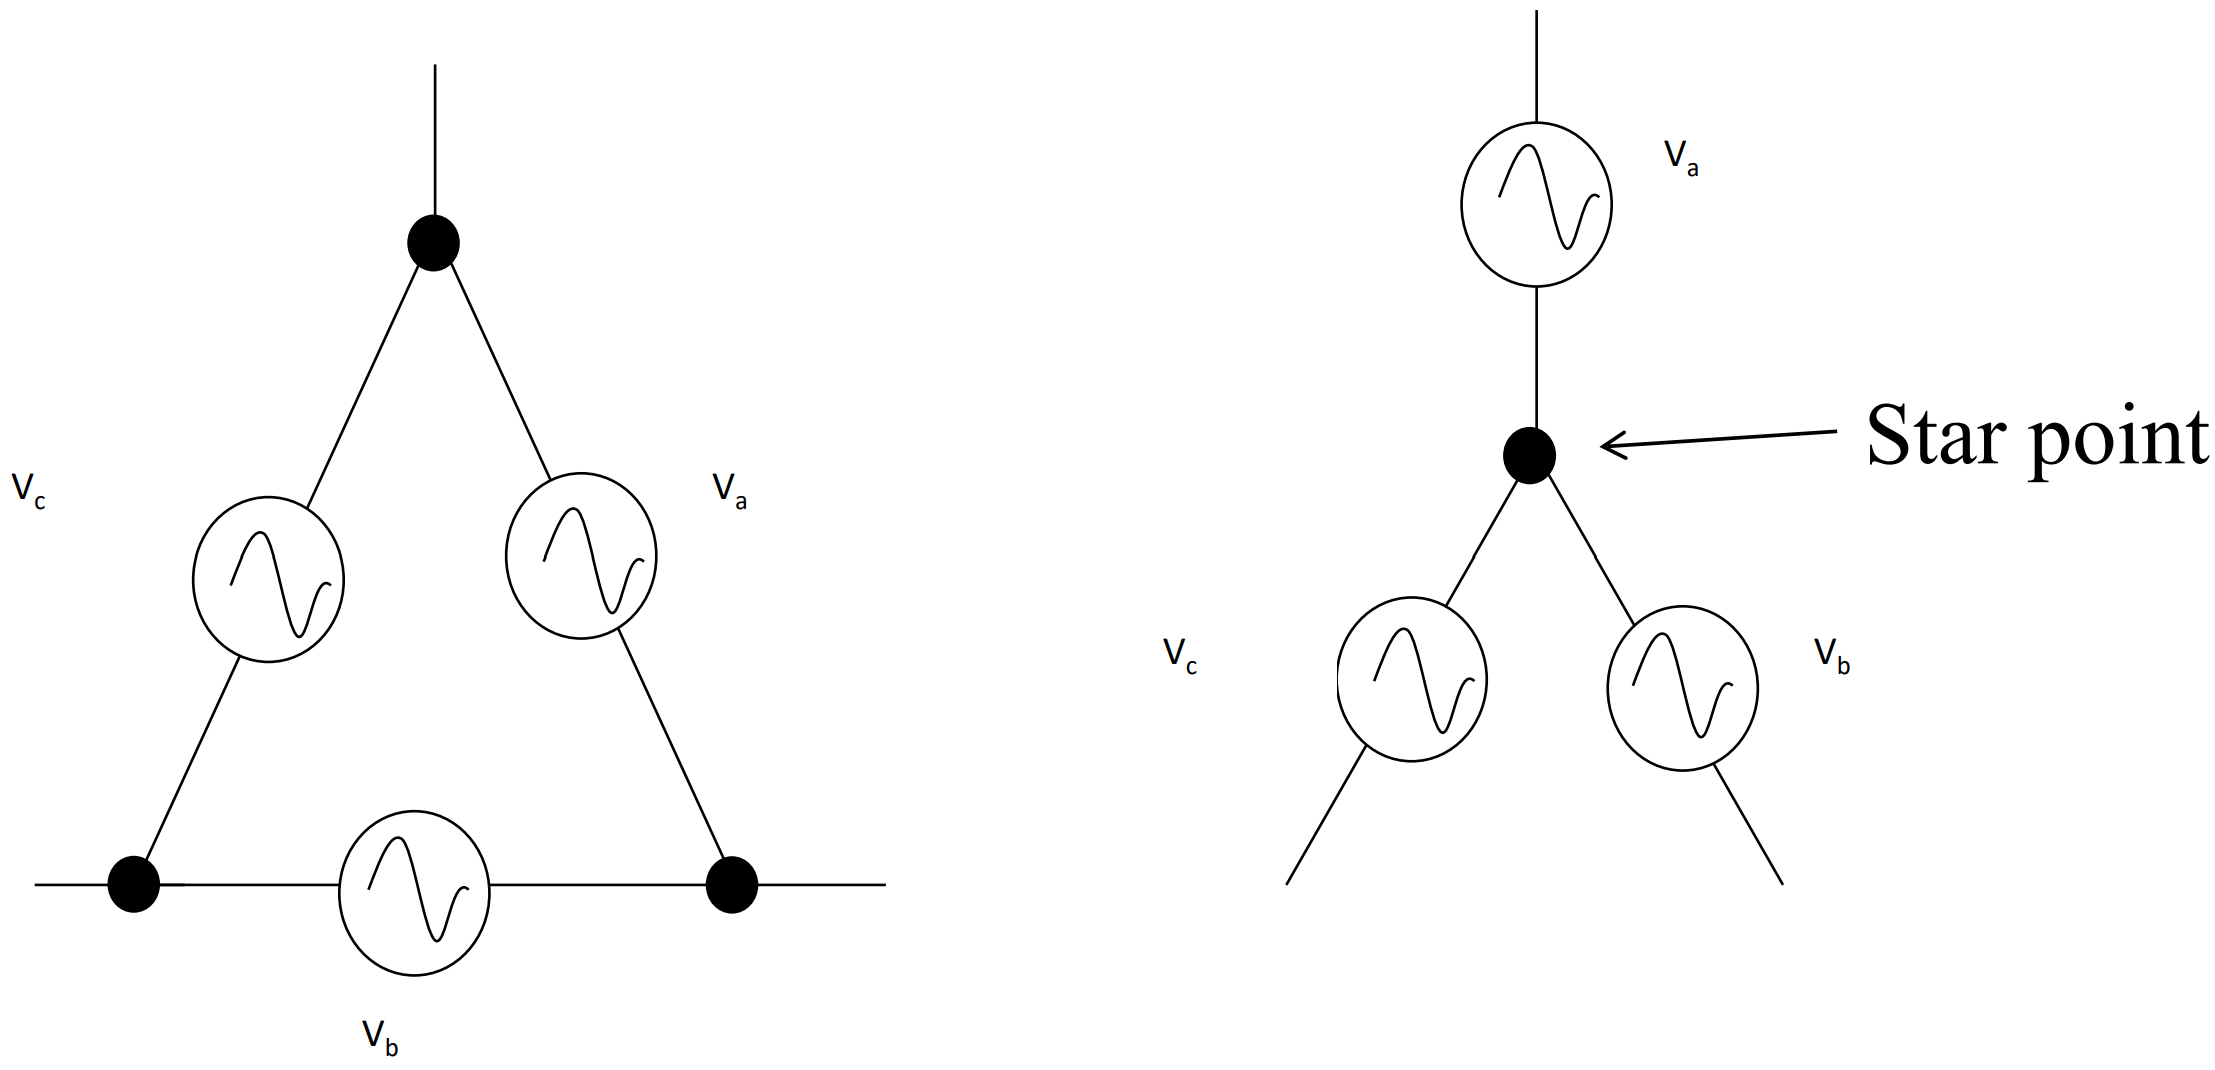
\includegraphics[width = \textwidth]{./img/figure7.png}
	\caption{Star and delta configurations.}
\end{figure}
\begin{figure}[H]
	\centering
	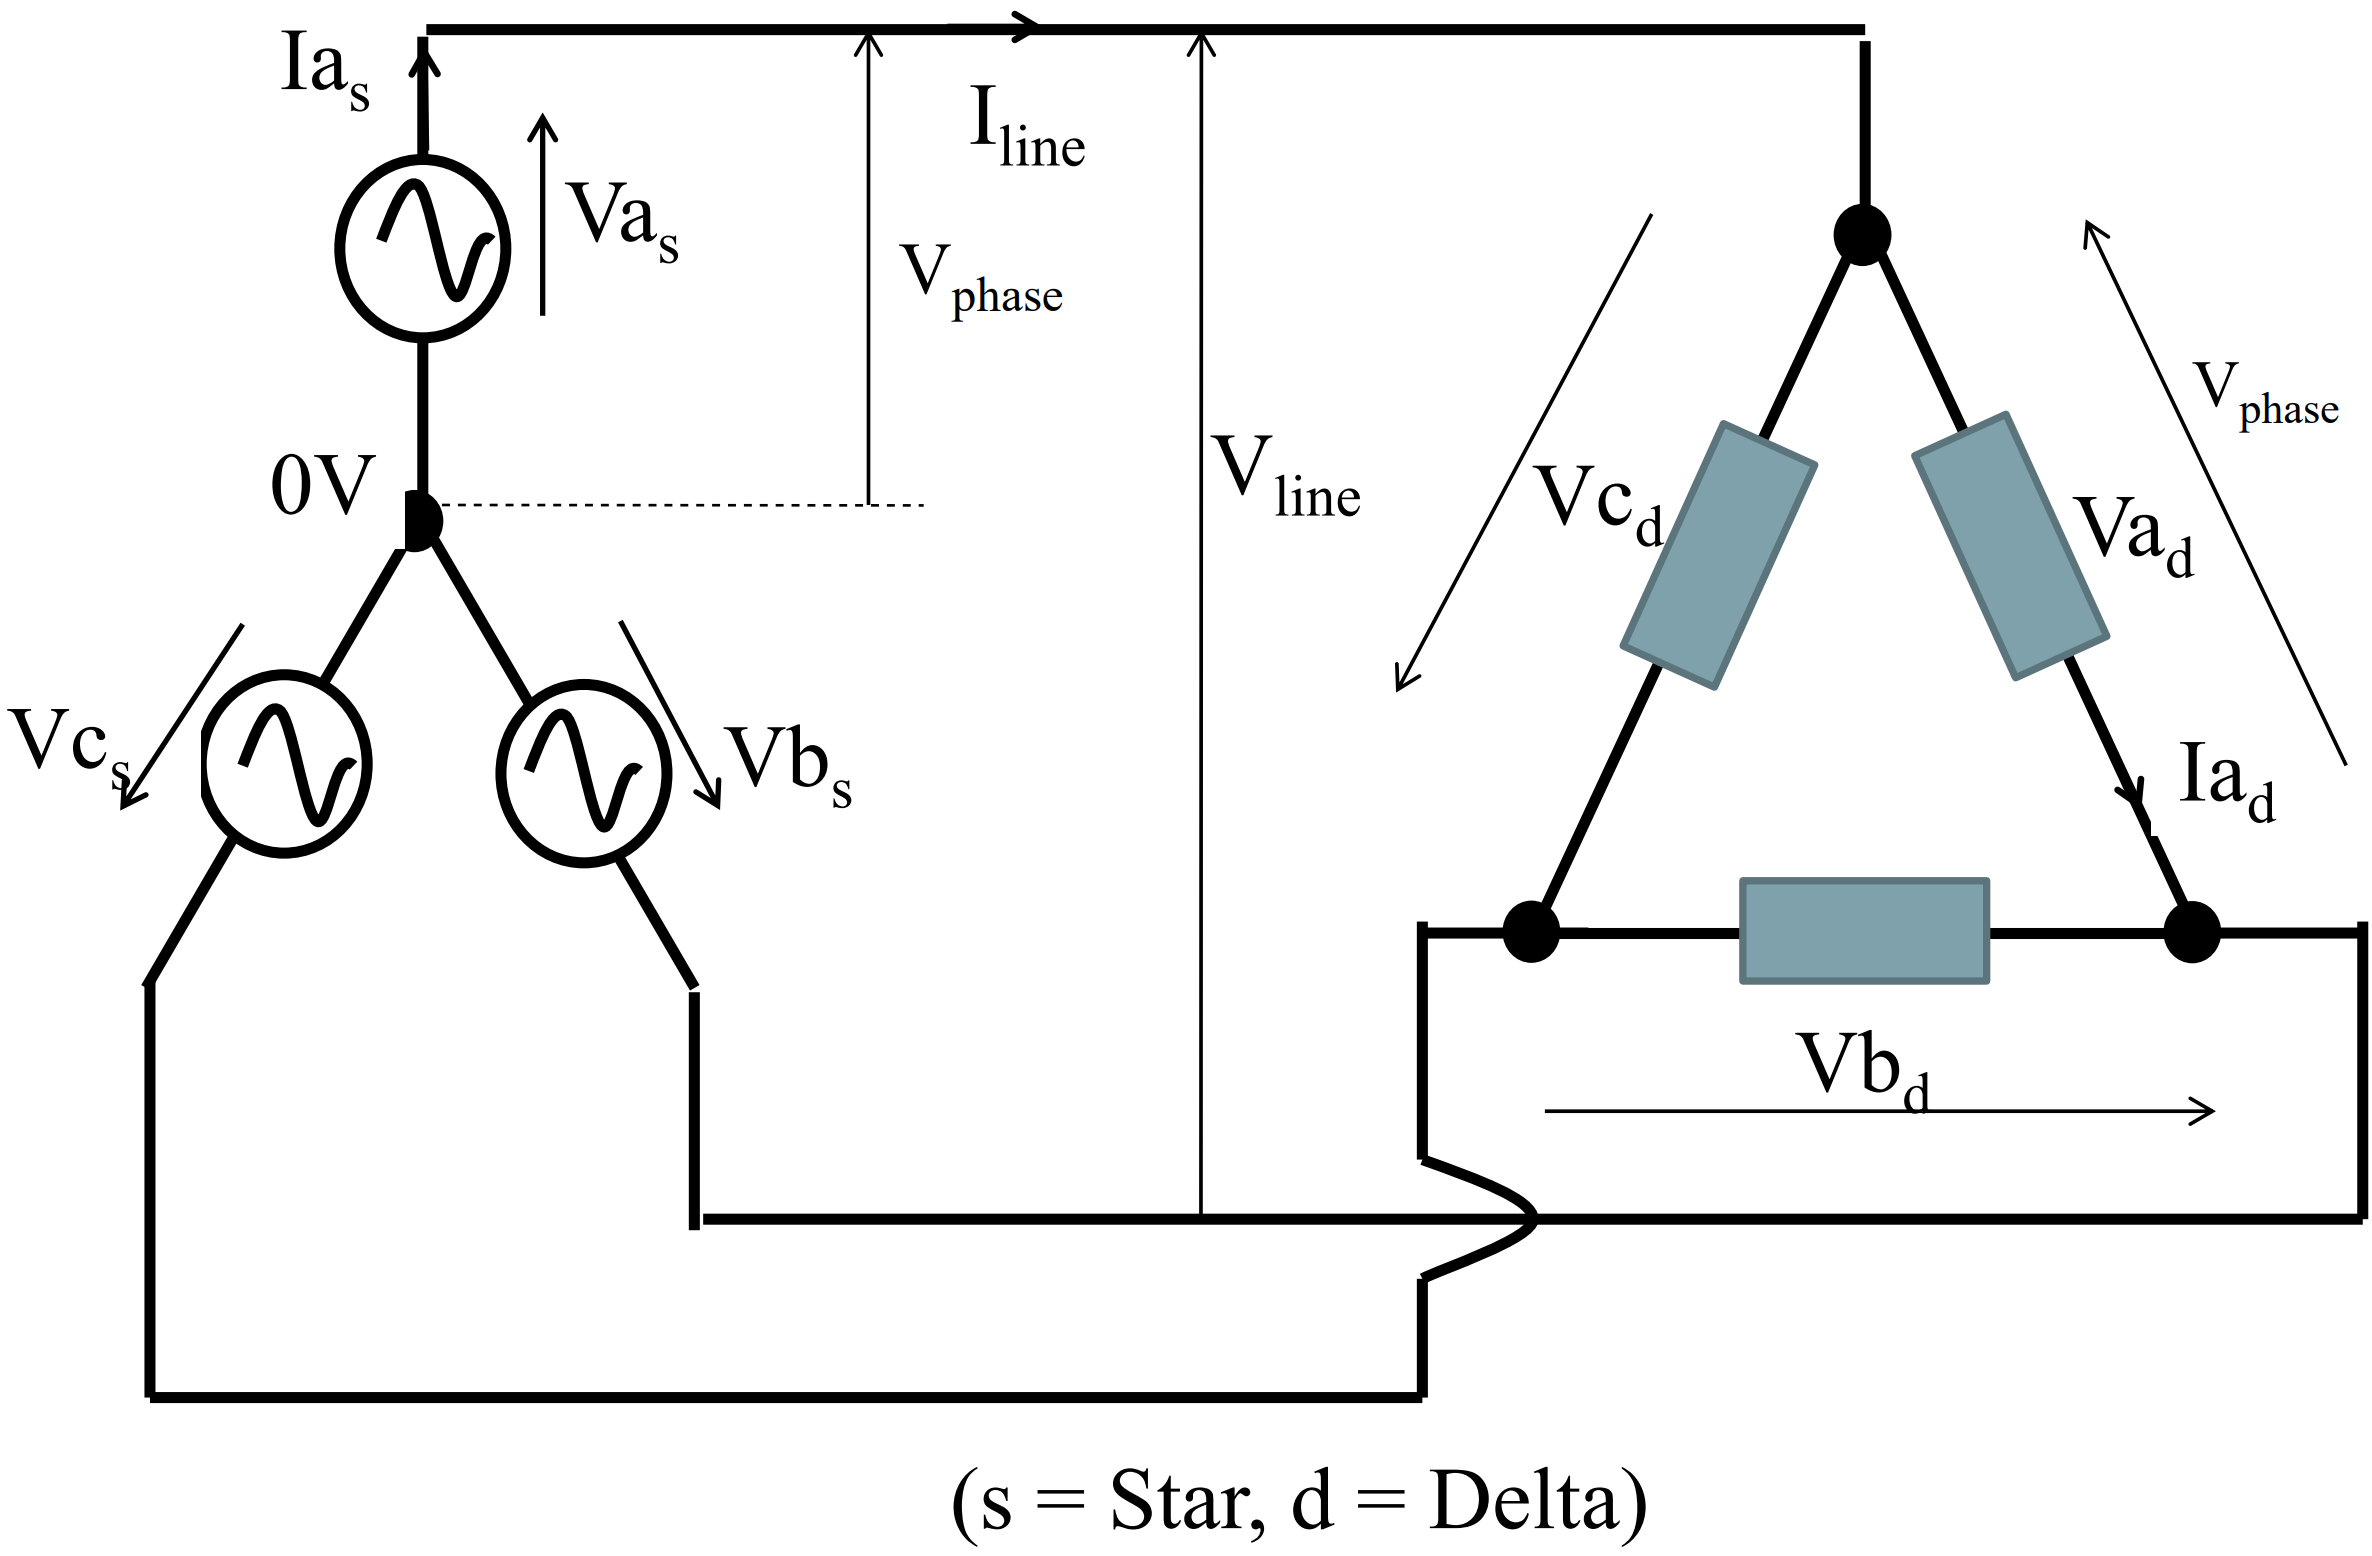
\includegraphics[width = \textwidth]{./img/figure8.png}
	\caption{Star generator and delta load.}
\end{figure}
\subsection{Phase and line voltages}
There are therefore two voltage types (either generated as a potential difference) when considering three-phase circuits. These are commonly known as the \textit{phase voltage} and \textit{line voltage}.

The phase voltages in the star-delta circuit are as follows:
\begin{itemize}
	\item $Vas$, $Vbs$, $Vcs$ for the star circuit
	\item $Vad$, $Vbd$, $Vcd$ for the delta circuit
\end{itemize}
The line voltages can be measured as follows:
\begin{align}
	Vab & = Vas - Vbs = Vad \\
	Vbc & = Vbs - Vcs = Vbd \\
	Vca & = Vcs - Vas = Vcd
\end{align}
and if the line voltages measure is reversed:
\begin{align}
	Vba & = Vbs - Vas = -Vad \\
	Vcb & = Vcs - Vbs = -Vbd \\
	Vac & = Vas - Vcs = -Vcd
\end{align}
Which is why a three-phase system is known as a six-pulse system - (important in power electronic systems).
\subsection{Relationships between star and delta}
For the delta arrangement:
\begin{align}
	V_p & = V_l                  \\
	I_p & = \frac{I_l}{\sqrt{3}}
\end{align}
For the star arrangement:
\begin{align}
	V_p & = \frac{V_l}{\sqrt{3}} \\
	I_p & = I_l
\end{align}
Where $I_p$ and $V_p$ are the phase currents and voltages and $I_l$ and $V_l$ are the line currents and voltages respectively. Note: Delta is also known as `mesh'; Star is also known as `Y'.
\subsection{Single-phase impedance triangle}
\begin{figure}[H]
	\centering
	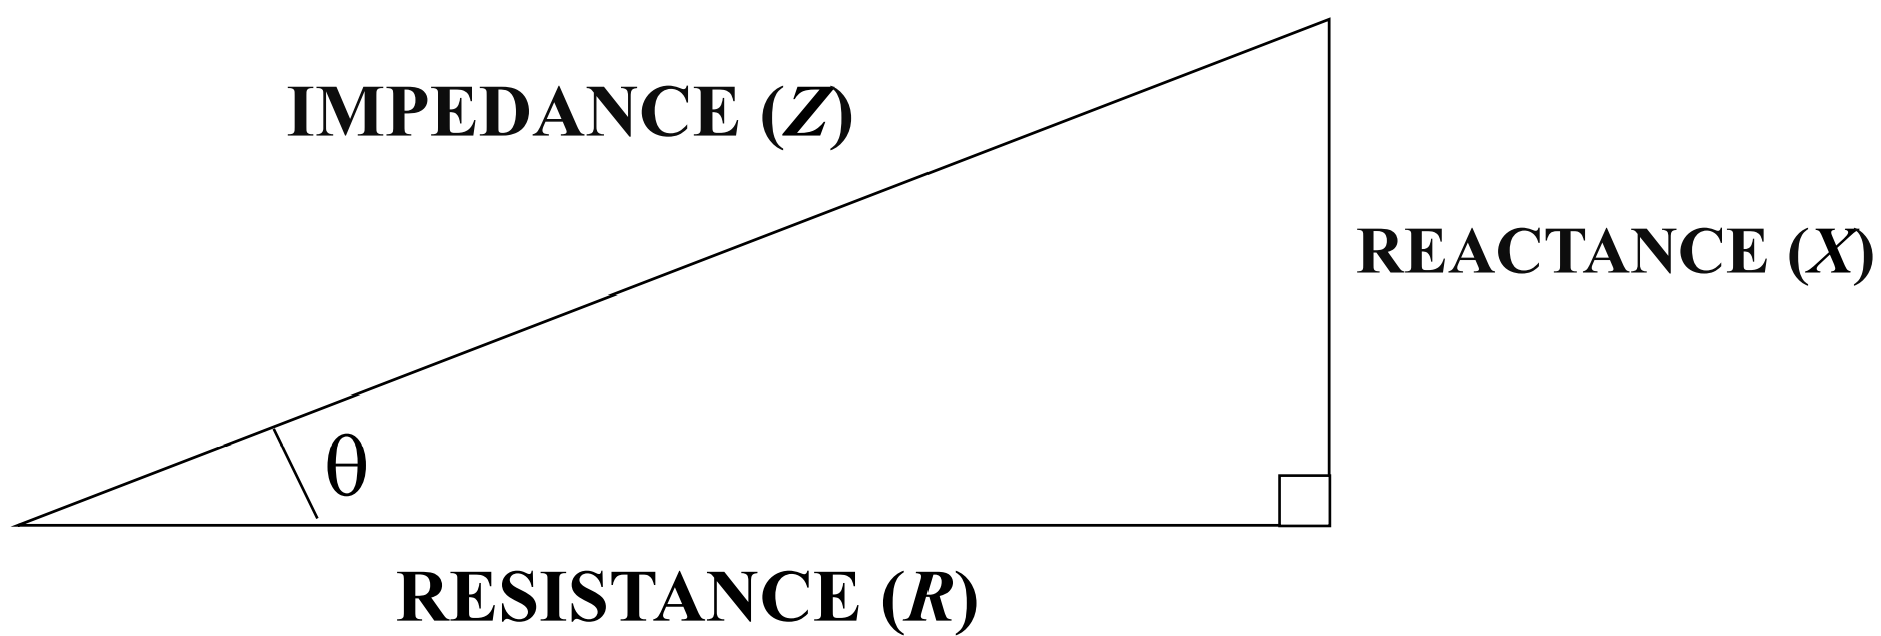
\includegraphics[width = 0.8\textwidth]{./img/figure9.png}
	\caption{Single-phase impedance triangle.}
\end{figure}
\begin{align}
	Z & = R + jX                                          \\
	  & = R + j\left(X_L - X_C\right)                     \\
	  & = R + j\left(\omega L - \frac{1}{\omega C}\right)
\end{align}
Where, $Z$ is impedance, $R$ is resistance, $X_L$ is inductive reactance, $X_C$ is capacitive reactance, $\omega$ is angular frequency ($2\pi f$).
\subsection{Single-phase power triangle}
\begin{figure}[H]
	\centering
	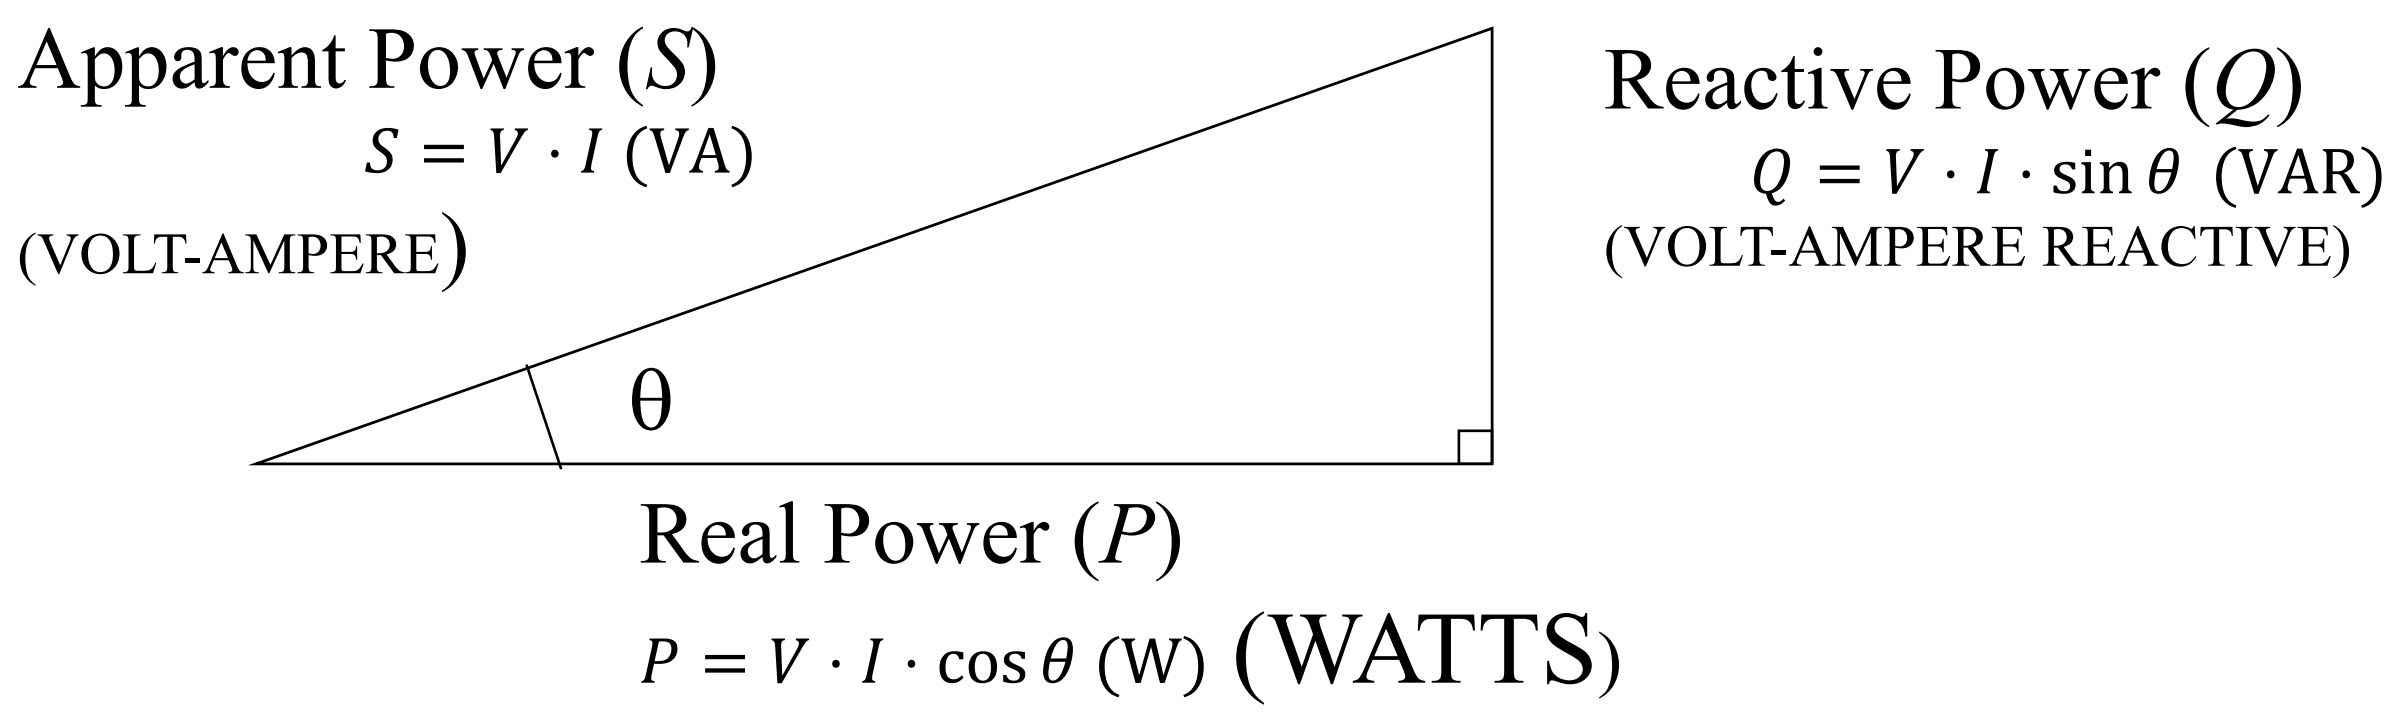
\includegraphics[width = 0.8\textwidth]{./img/figure10.png}
	\caption{Single-phase power triangle.}
\end{figure}
\begin{itemize}
	\item Real power ($P$) is the power that can be put into or taken from the electrical system and is measured in Watts (\si{\watt}).
	\item Reactive power ($Q$) is the power that circulates in the electrical system and is measured in Volt-Ampere-Reactive (VAR).
	\item Apparent power ($S$) is what is apparent from the product of voltage and current and is measured in Volt-Amperes (VA).
\end{itemize}
\subsection{Three-phase power}
Since $V$ in the star circuit and $I$ in the delta circuit is subject to change simply by dividing by $\sqrt{3}$, whilst the other variable $I$ and $V$ in star and delta respectively remain unchanged. Hence we get:
\begin{gather}
	P = \sqrt{3} \cdot I_{line} \cdot V_{line} \cdot \cos \theta
\end{gather}
For apparent power ($S$) and reactive power ($Q$) we have:
\begin{align}
	S & = \sqrt{3} \cdot I_{line} \cdot V_{line}                   \\
	Q & = \sqrt{3} \cdot I_{line} \cdot V_{line} \cdot \sin \theta
\end{align}
\subsection{Student Activity}
Three coils each of resistance \SI{5}{\ohm} and inductive reactance of \SI{10}{\ohm} are connected in (a) star and (b) delta across a \SI{440}{VRMS} three-phase (line) supply.

If each coil has a capacitor connected in parallel having capacitive reactance of \SI{20}{\ohm} then calculate the line and phase currents and the total power absorbed.
\section{Per Unit (PU) System}
\subsection{Electrical line diagram to Impedance diagram}
\begin{itemize}
	\item The \textit{`electrical line diagram'} - a schematic which allows an understanding of equipment and system arrangements.
	\item The \textit{`impedance diagram'} - a schematic which allows an understanding of the equipment and system impedances.
	\item The layout of both the `electrical line diagram' and `impedance diagram' should be similar but in the `impedance diagram' all equipment and lines are replaced with impedances.
	\item All impedances will need to be calculated to a \textit{common base} - hence use of a per unit system.
\end{itemize}
\subsection{Simple equivalent impedances}
For the purposes of steady-state analysis the Electrical Line Diagram is converted to an `Impedance Line Diagram' where the equipment is represented as an `Equivalent Impedance'. Typical \textit{simple} impedances representing equipment are: (note: not all $R$, $L$ and $C$ values may be given).
\begin{figure}[H]
	\centering
	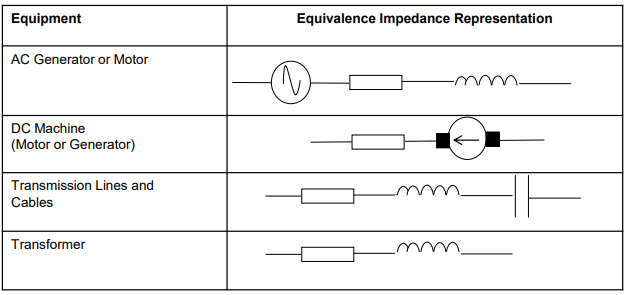
\includegraphics[width = \textwidth]{./img/figure11.png}
	\caption{Equivalent Impedance Representations.}
\end{figure}
\subsection{How manufacturers of electrical equipment specify ratings}
Manufacturers of electrical equipment would usually specify electrical equipment as follows:

e.g. A synchronous generator
\begin{itemize}
	\item S = 10 MVA (value of apparent power)
	\item V = 3.3 kV (line voltage rating of the equipment)
	\item Phase = 3 (number of phases)
	\item PF = 0.8 (usual value of power factor of equipment)
	\item N = 1500 rpm (design speed of rotation)
	\item F = 50 Hz (frequency of the alternating current \& voltage)
	\item X = 0.14 (Reactance given as a pu value or as a \%)
	\item Connection = star (stator windings)
\end{itemize}
\subsection{The per unit system}
In Electrical Power System Analysis the per unit system is the preferred method for analysing circuit behaviour rather than the standard SI system of units (Watts, Volts, Amperes, etc.)

The advantages of the per unit system are:
\begin{itemize}
	\item Computations for power systems have several voltage levels because of connected transformers is very cumbersome when using the SI system because values need to be referred across the transformer turns ratio. The per unit system (overcomes or simplifies) this problem.
	\item All powers, voltage, currents and impedances are expressed as per unit values of specified base values. This means they are easily compared with one another which is very helpful for equipment specification and selection and in power system design and its analysis.
\end{itemize}
\subsection{Values in per unit system}
In the per unit system five base values are needed. These are \textbf{power, current, voltage, impedance} and \textbf{power factor}. It is necessary to choose two base values and to calculate two base values.

Usually the base values defined are:
\begin{itemize}
	\item the Apparent Power (Base\_VA)
	\item Voltage (Base\_V)
\end{itemize}
Power Factor is already expressed in per unit form. Once the base values are calculated then `actual values' in the circuit can be expressed in per unit form.
\subsection{Three-Phase system PU conversion}
\subsubsection{Step one}
The per unit relationships for Base\_VA and Base\_V are define and Base\_I and Base\_Z are calculated:
\begin{align}
	\textrm{Base\_VA} & = \textrm{Defined by Engineer}                              \\
	\textrm{Base\_V}  & = \textrm{Defined by Engineer}                              \\
	\textrm{Base\_I}  & = \dfrac{\textrm{Base\_VA}}{\sqrt{3}\cdot \textrm{Base\_V}} \\
	\textrm{Base\_Z}  & = \dfrac{\textrm{Base\_V}}{\textrm{Base\_I}}
\end{align}
\subsubsection{Step two}
Having calculated the Base Values, these are then defined as being 1 per unit values:
\begin{itemize}
	\item Base\_V = 1 per unit Voltage
	\item Base\_VA = 1 per unit Apparent Power
	\item Base\_I = 1 per unit Current
	\item Base\_Z = 1 per unit Impedance
\end{itemize}
\subsubsection{Step three}
In the circuit all apparent powers, voltage, currents and impedances are expressed as per unit values:
\begin{align}
	\textrm{Per\_Unit\_S} & = \dfrac{\textrm{Actual\_Value\_S}}{\textrm{Base\_S}} \\
	\textrm{Per\_Unit\_V} & = \dfrac{\textrm{Actual\_Value\_V}}{\textrm{Base\_V}} \\
	\textrm{Per\_Unit\_I} & = \dfrac{\textrm{Actual\_Value\_I}}{\textrm{Base\_I}} \\
	\textrm{Per\_Unit\_Z} & = \dfrac{\textrm{Actual\_Value\_Z}}{\textrm{Base\_Z}}
\end{align}
\subsubsection{Step four}
Sometimes parameters e.g. Z are already expressed in per unit form rather than as SI units but have been calculated to a different base (S and V). These can be converted as follows:
\begin{gather}
	\left(\textrm{Per\_Unit\_Z}\right)_{\textrm{new\_base}} = \dfrac{\left(\textrm{Base\_VA}\right)_{\textrm{new\_base}}}{\left(\textrm{Base\_VA}\right)_{\textrm{old\_base}}} \cdot \dfrac{\left(\textrm{Base\_V}\right)^2_{\textrm{old\_base}}}{\left(\textrm{Base\_V}\right)^2_{\textrm{new\_base}}} \cdot \left(\textrm{Per\_Unit\_Z}\right)_{\textrm{old\_base}}
\end{gather}
Some manufacturers and engineers prefer to work with the percentage system rather than the per unit system which of course is a simple matter of mulitplying by 100/ Equipment manufacturers use a machine's own S and V to determine base values from which Z pu is then calculated.
\subsection{Example PU system conversion}
\subsubsection{Single Line Diagram}
\begin{figure}[H]
	\centering
	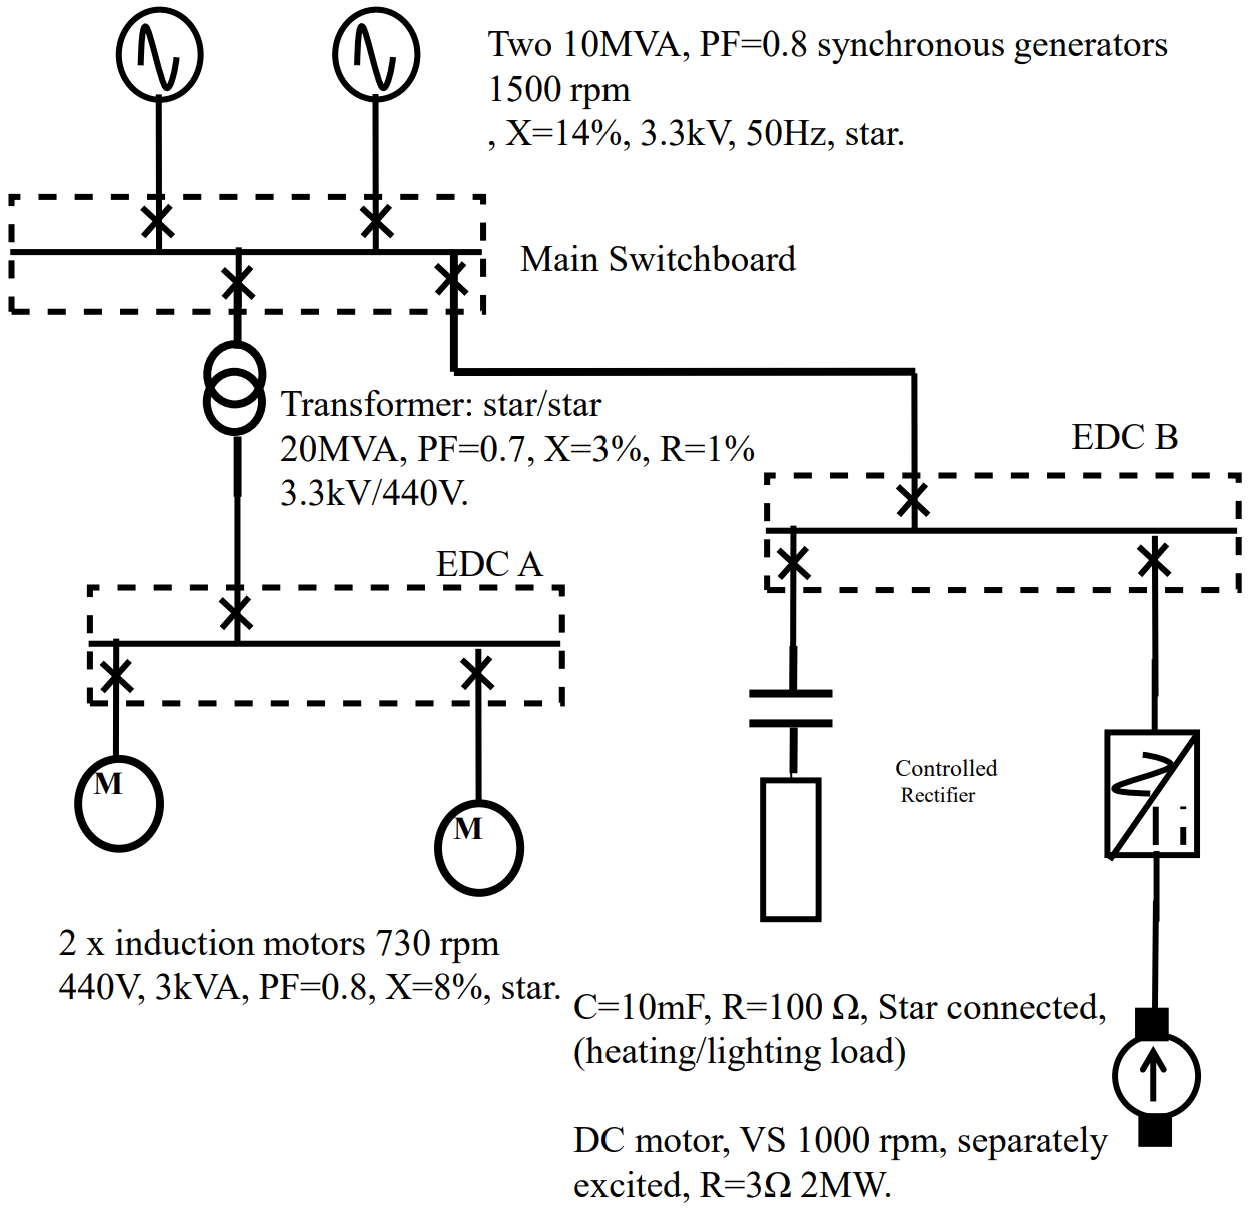
\includegraphics[width = \textwidth]{./img/figure12.png}
	\caption{Single Line Diagram.}
\end{figure}
\subsubsection{Step one - calculating the base current and base impedance}
Selecting 10 MVA as Base\_S and 3.3 kV as Base\_V (because it seems sensible considering the generators) then we have:
\begin{align}
	\textrm{Base\_I} & = \dfrac{10 \time 10^6}{\sqrt{3}\times 3.3 \times 10^6} = \SI{1749.5}{\ampere} \\
	\textrm{Base\_Z} & - \dfrac{3.3\times 10^3}{1749.5} = \SI{1.886}{\ohm}
\end{align}
\subsubsection{Step two - defininng 1 p.u. values}
\begin{itemize}
	\item \SI{3.3e3}{\volt} = 1 per unit Voltage = 1 pu V
	\item \SI{10e6}{VA} = 1 per unit Apparent Power = 1 pu S
	\item \SI{1749.5}{\ampere} = 1 per unit Current = 1 pu A
	\item \SI{1.886}{\ohm} = 1 per unit Impedance = 1 pu Z
\end{itemize}
Sometimes \% values are preferred by some engineers i.e. 1 pu = 100\%
\subsubsection{Step three - converting impedances expressed in SI units to per unit form}
The only `actual values' i.e. expressed in SI units, are the heating load and the DC machine:

For the lighting/heating load:
\begin{gather}
	-jXC = -j \left( \dfrac{1}{2\pi\cdot 50 \cdot 10 \times 10^{-3}}\right) = -j0.318\\
	-jXC = \dfrac{-j0.318}{1.886} = -j0.168\, \si{pu}\\
	R = \dfrac{100}{1.886} = 53.022\,\si{pu}
\end{gather}
For DC motor:
\begin{gather}
	R = \dfrac{3}{1.886} = 1.591\, \si{pu}\\
	S = P + \dfrac{2}{10} = 0.2\, \si{pu}
\end{gather}
\subsubsection{Step four - converting impedances expressed in per unit form to another base}
For the synchronous generators:
\begin{gather}
	S = \dfrac{10}{10} = 1\, \si{pu}\\
	V = \SI{3.3}{\kilo\volt} = 1\, \si{pu}\\
	X = \dfrac{14}{100} = 0.14\, \si{pu}\\
	PF = 0.8\, \si{pu}
\end{gather}
For the transformer:
\begin{gather}
	S = \dfrac{20}{10} = 2\, \si{pu}\\
	X = \dfrac{3}{100} \times \dfrac{10}{20} = 0.015\,\si{pu}\\
	R = \dfrac{1}{100} \times \dfrac{10}{20} = 0.005\,\si{pu}\\
	PF = 0.7\,\si{pu}
\end{gather}
For the induction motors:
\begin{gather}
	S = \dfrac{3}{10000} = 0.0003\,\si{pu} \\
	X = \dfrac{8}{100} \times \dfrac{10000}{3} = 266.667\,\si{pu} \\
	PF = 0.8
\end{gather}
\subsubsection{Step five - drawing the impedance diagram}
\begin{figure}[H]
	\centering
	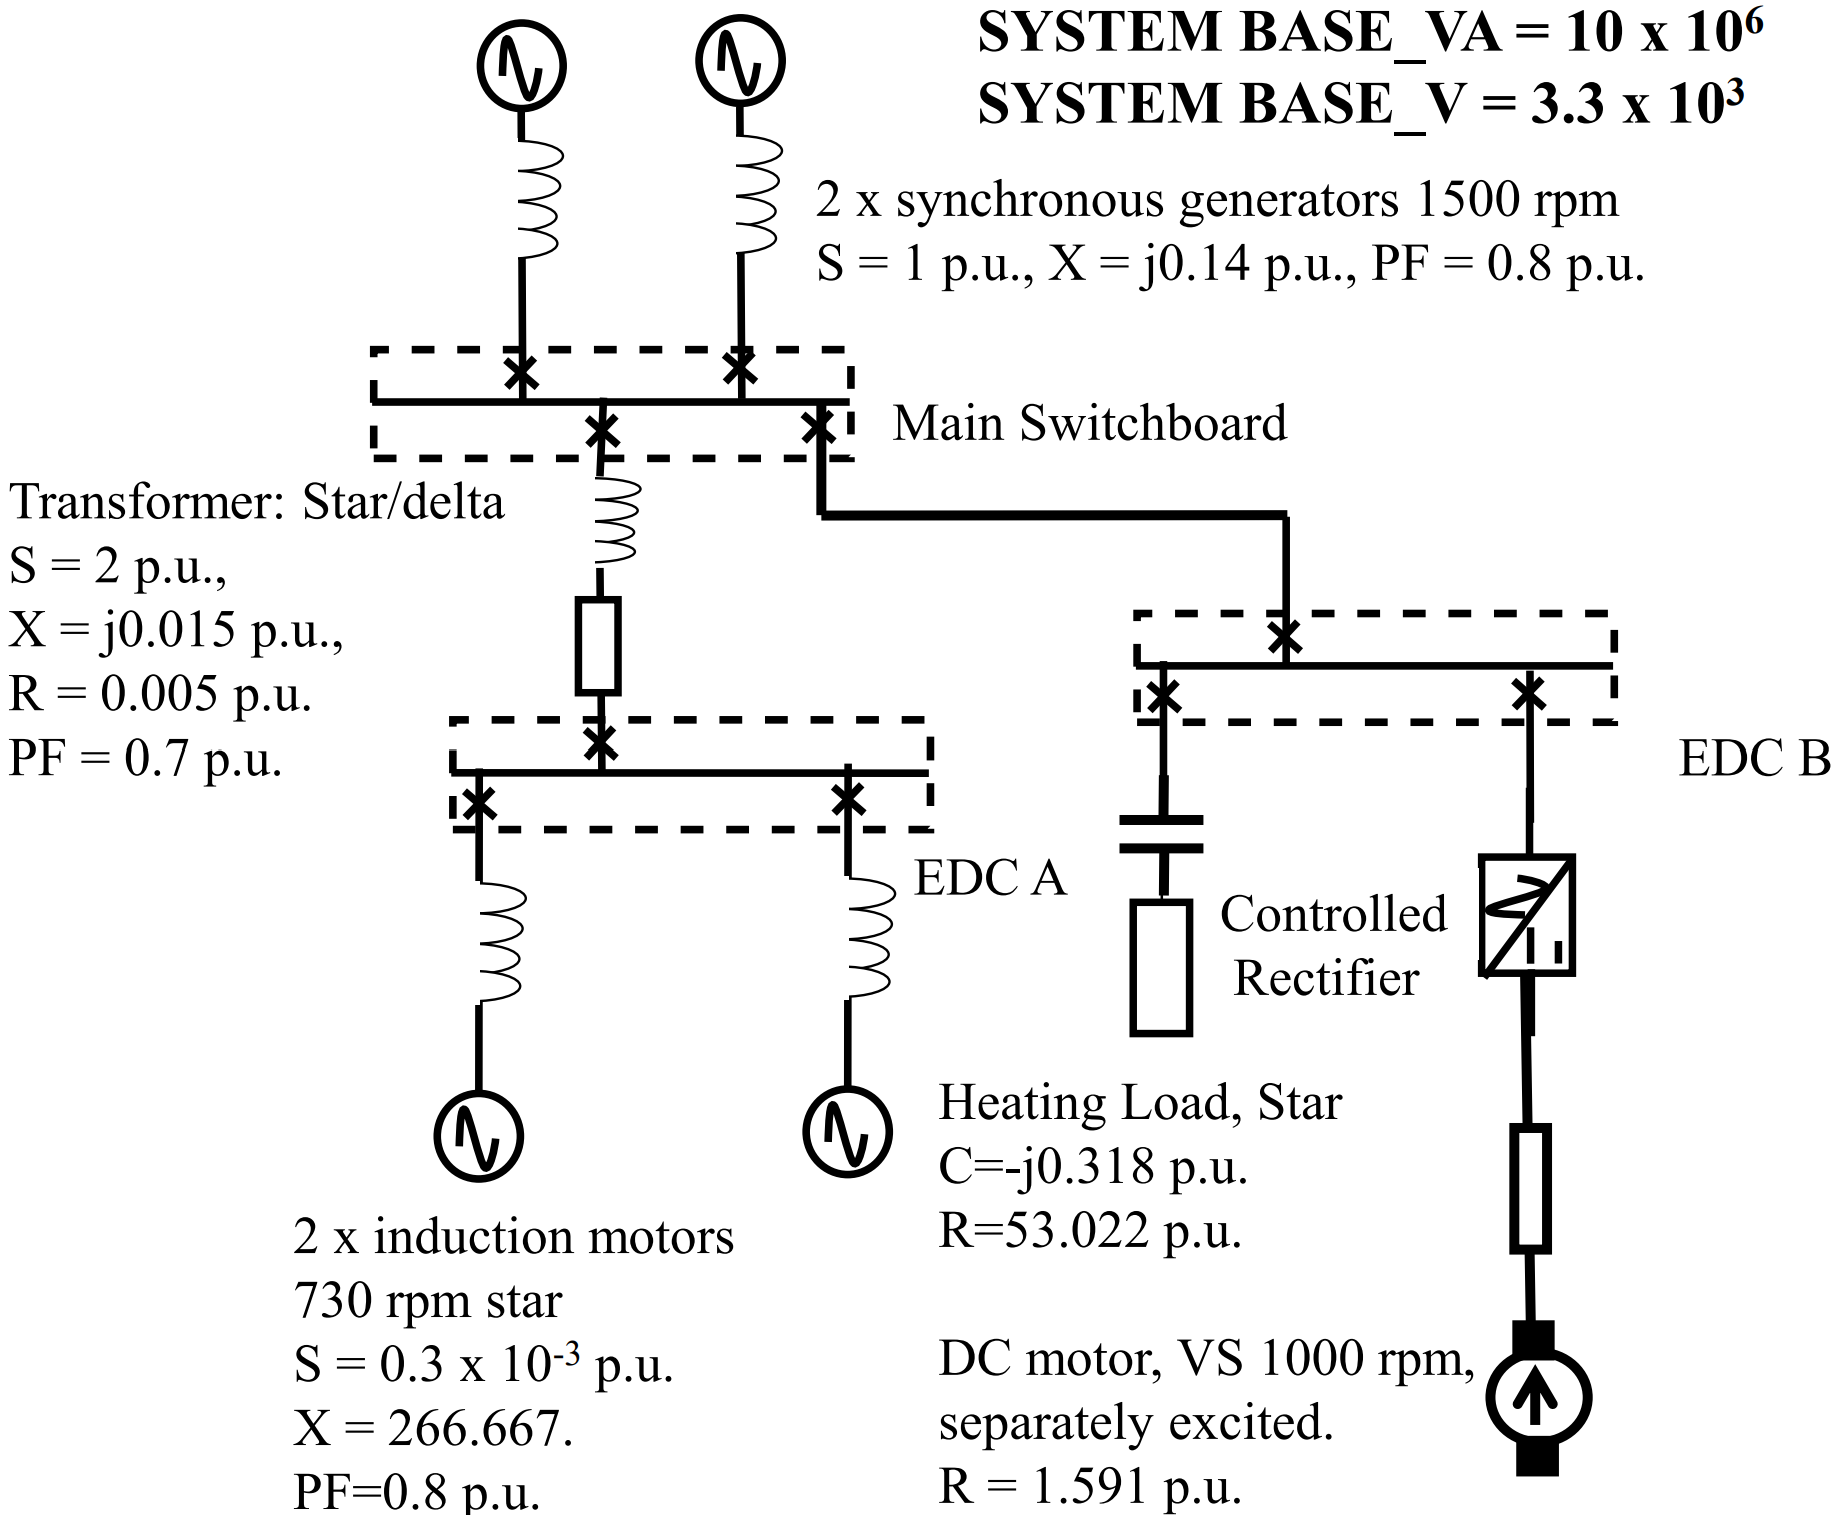
\includegraphics[width = \textwidth]{./img/figure13.png}
	\caption{Impedance Diagram.}
\end{figure}
\subsection{Reactance diagram}
The reactance diagram is a modification to the impedance diagram where only per unit reactances are shown. In a reactance diagram all resistances are ignored. The reactance diagram is useful because it allows `first pass' calculations to be made in a power system without too much mathematical complexity due to having ($R \pm jX$).
\begin{figure}[H]
	\centering
	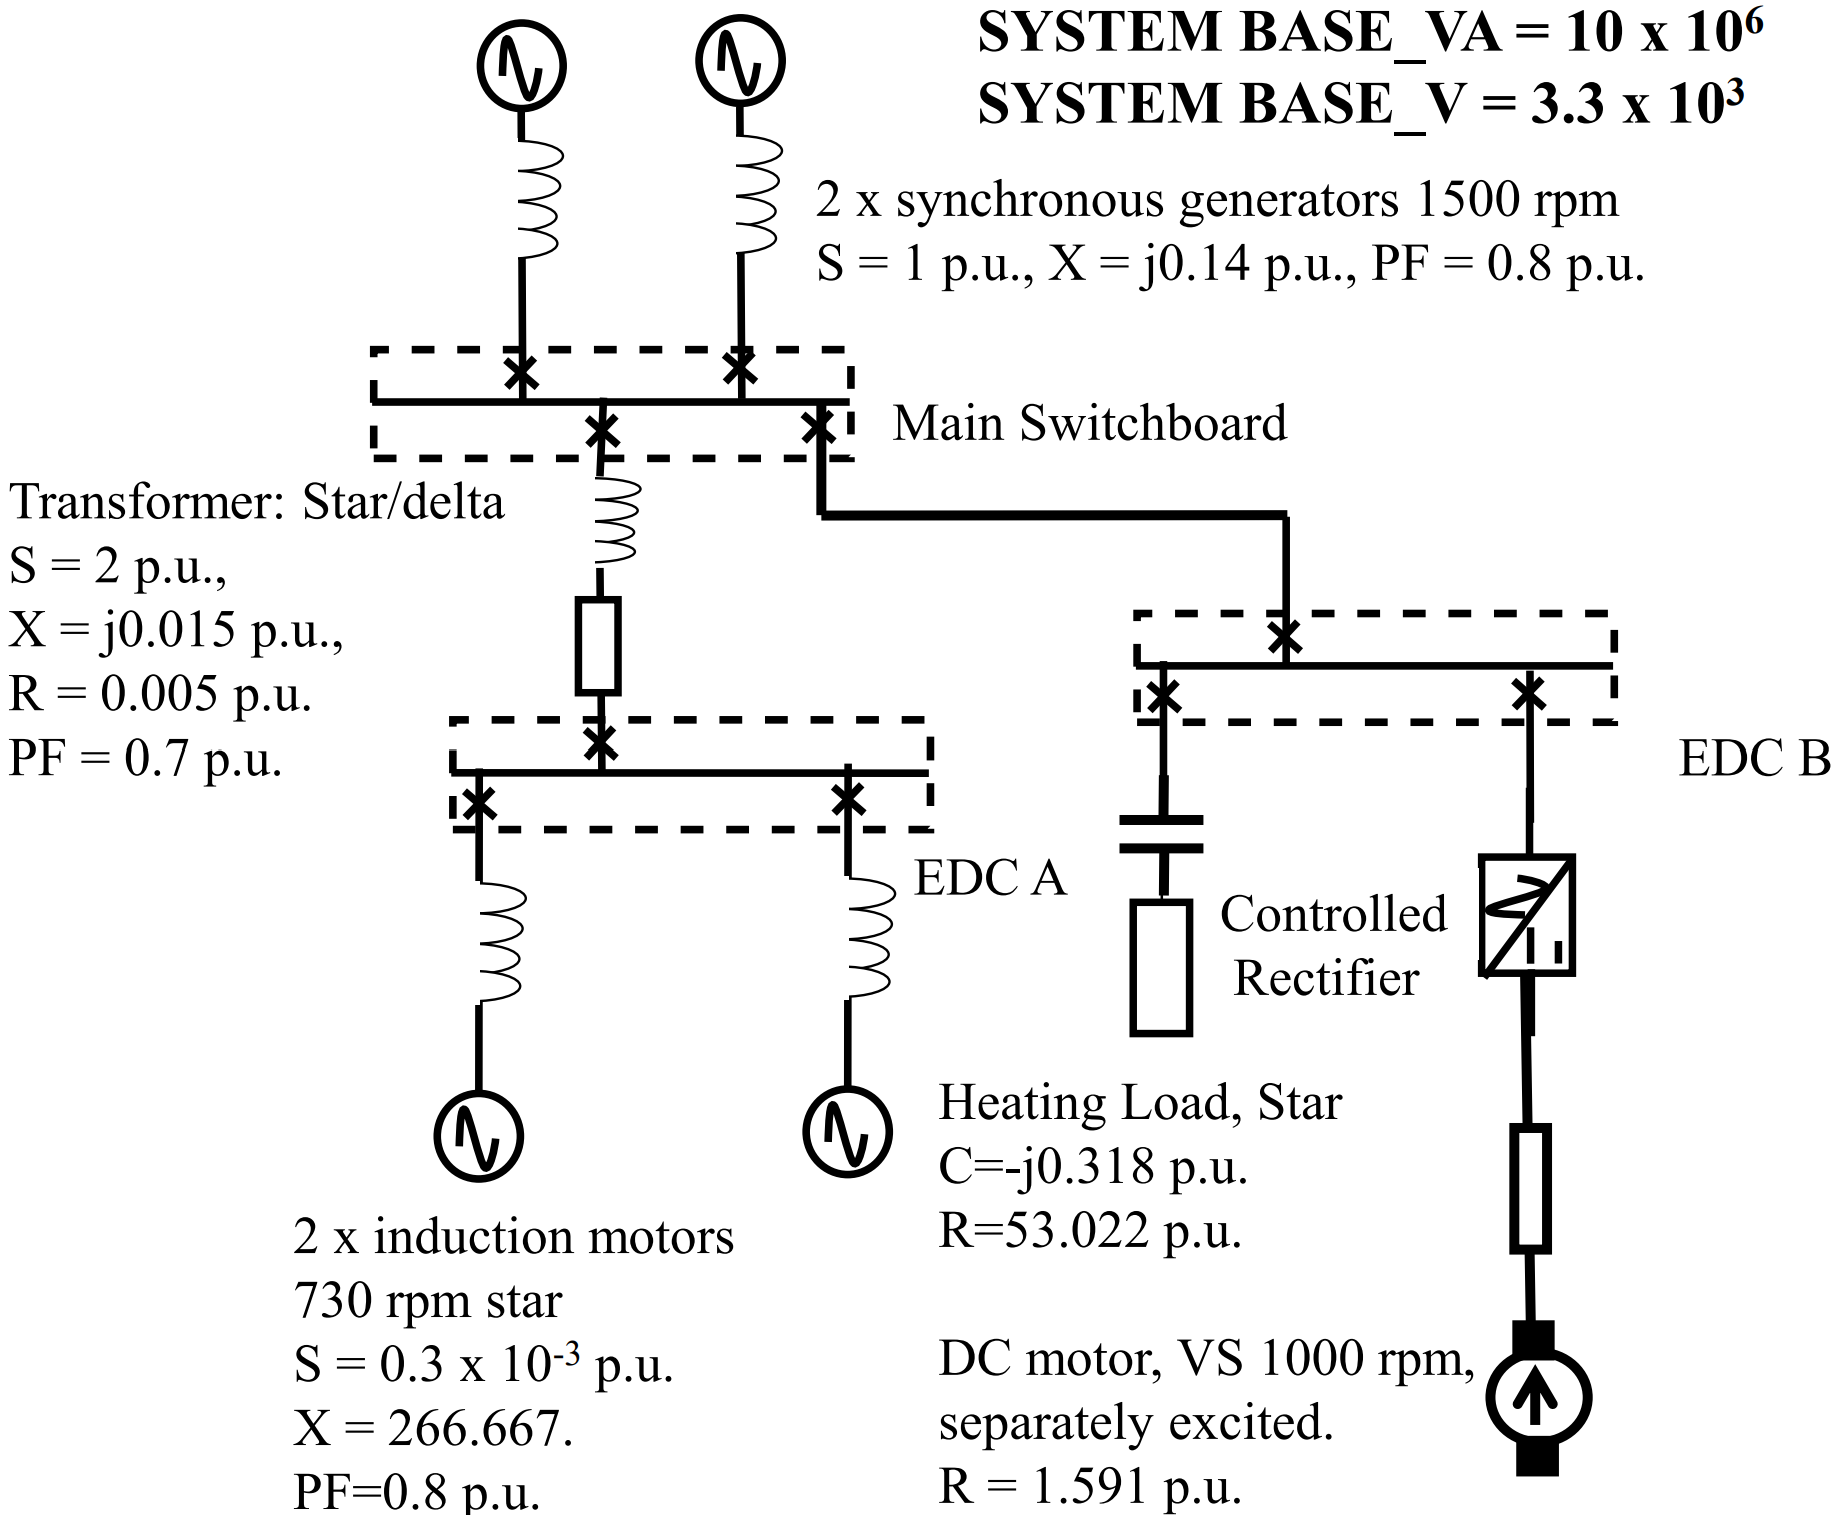
\includegraphics[width = \textwidth]{./img/figure13.png}
	\caption{Reactance Diagram.}
\end{figure}
\subsection{Impedance and reactance diagrams}
Converting the electrical line diagram to an impedance diagram or reactance diagram is essential for:
\begin{itemize}
	\item Potential difference (voltage drop) calculations
	\item Current flows in cables/lines
	\item Calculations of losses
	\item Power flows around an electrical system
	\item Understand transient effects
	\item Calculate fault level and fault currents
	\item Waveform distortion and its penetration
	\item Impacts when adding new equipment to the network
\end{itemize}
\section{Summary}
The per unit system allows powers, voltages, currents and impedances to be expressed relative to each other. This allows the designer to understand the relationships between different parts of the circuit.

Using the per-unit transformer model eliminates the need to scale quantities by the transformer turns ratio, thus eliminating a common source for error in electrical calculations.














\documentclass[class=report, crop=false, 12pt,a4paper]{standalone}
\usepackage{enumitem}
\usepackage{multicol}
\usepackage{graphicx}
\usepackage{float}
\usepackage{amsmath}
\usepackage{amssymb}
\usepackage{mathtools}
\usepackage{siunitx}
\usepackage{commath}
\usepackage{array}
\usepackage{natbib}
\usepackage[a4paper,width=150mm,top=25mm,bottom=25mm]{geometry}
\setlength{\parindent}{0pt}
\setlength{\parskip}{1em}
\raggedbottom
\begin{document}
\chapter{Using the Impedance Diagram}
\begin{itemize}
	\item Using impedance diagrams for load flows
	\item Using impedance diagrams for fault calculations
\end{itemize}
\begin{quote}
	By the end of this synchronous session you should be comfortable with how impedance diagrams can be used to calculate load flows and perform fault calculations in an electrical power system
\end{quote}
\section{Load Flow Calculation}
\subsection{Load flow}
\begin{itemize}
	\item In an electrical power system currents flow from generators to loads via a transmission/distribution system therby permitting `load (power) flows'
	\item If a system is at steady-state then currents and power flows would be stable
	\item If there is a change in the system e.g. suddenly and additional load is connected, then there will be a change to currents and load flow
	\item An electrical system cannot change instantaneously from one state to another. The generators for example cannot instantaneously change the supply of power at the point load changes. There will be a transient period
\end{itemize}
\subsection{Load flow analysis example}
\begin{figure}[H]
	\centering
	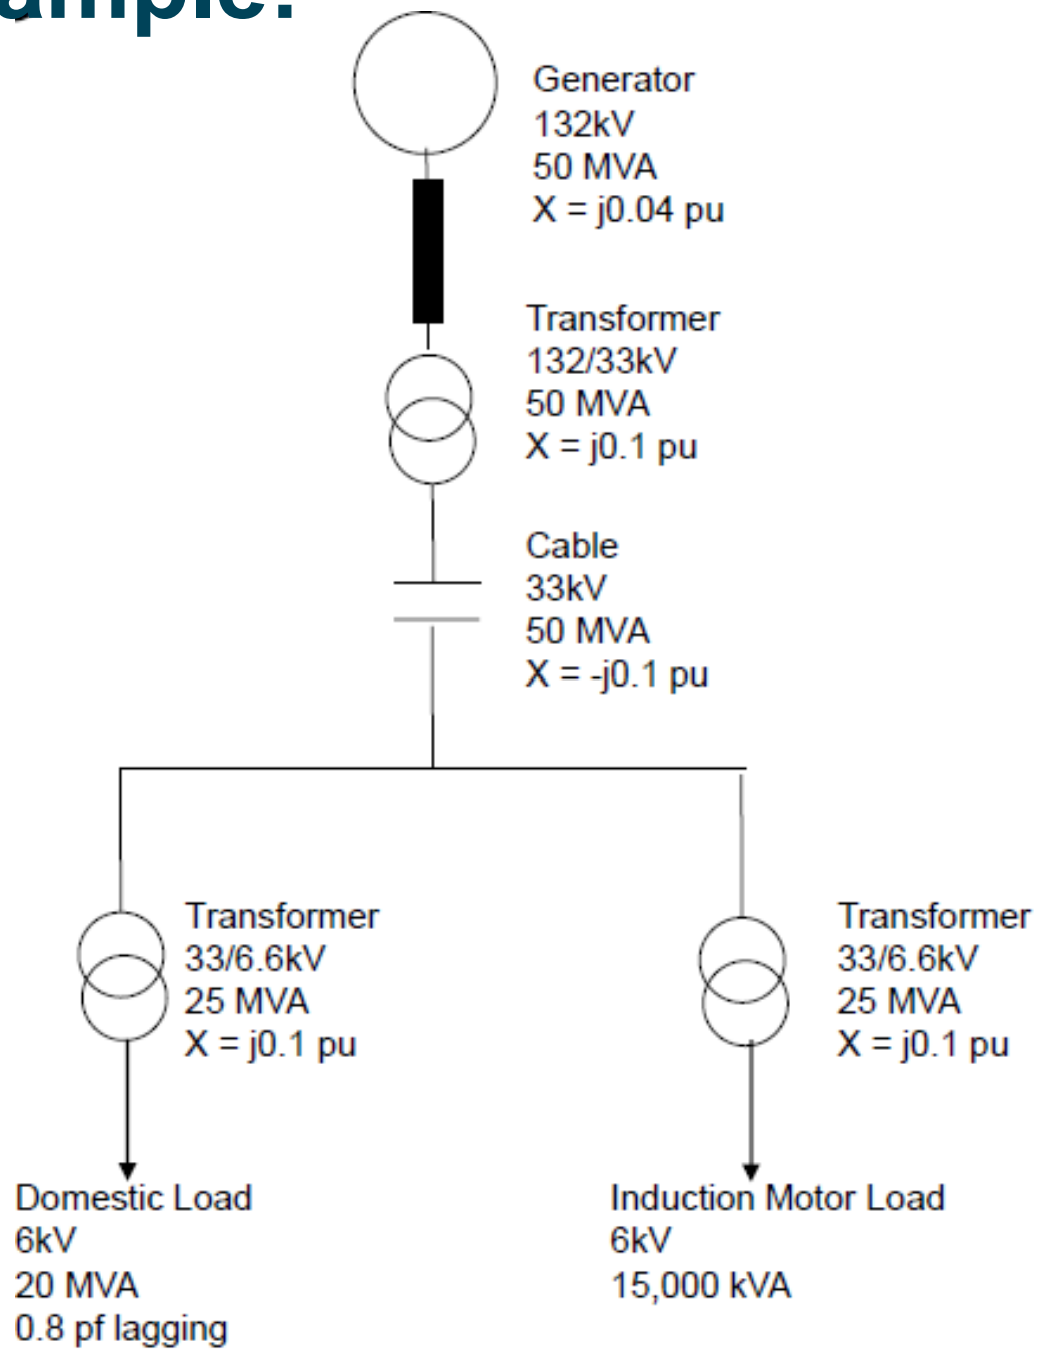
\includegraphics[width = 0.9\textwidth]{../img/figure15.png}
	\caption{Single Line Diagram.}
\end{figure}
A \SI{132}{kV} supply feeds two loads; a group of domestic consumers and a group of induction motors which on starting consume five times rated (or design) full load current at zero power factor lagging.
\subsubsection{Part a}
Convert the single line diagram into an impedance diagram. We will select a base S of \SI{50}{MVA} and \SI{33}{kV} as the base V. The values selected can be different but must be stated by the designer.
\begin{figure}[H]
	\centering
	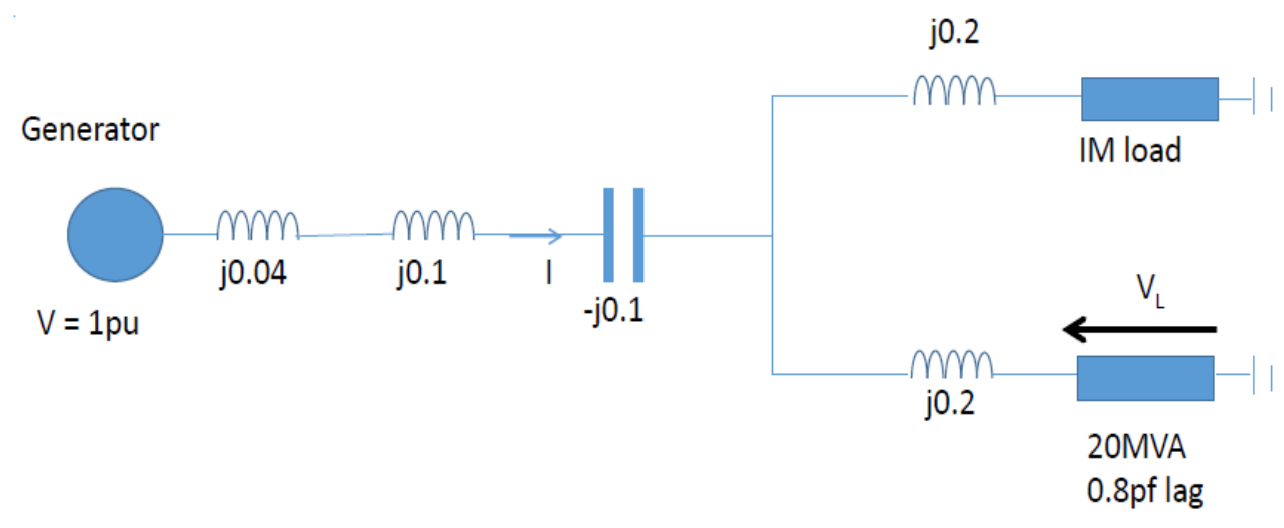
\includegraphics[width =  \textwidth]{../img/figure16.png}
	\caption{Single Line Diagram.}
\end{figure}
Here is the Impedance Diagram of the Single Line Diagram where all the impedances have been changed into per unit values on a \SI{50}{MVA} base.
\subsubsection{Part b}
Calculate the voltage at the domestic busbars prior to induction motor start. 
\begin{itemize}
	\item The induction motor load is open circuit so all current flowing from the generator will flow to the domestic load i.e. steady state
	\item To determine the voltage at the domestic busbar prior to the induction motor start then the equation for $V_L = 1 - IZ$ can be used, where:
	\begin{itemize}
		\item $V_L$ is the domestic voltage
		\item 1 is the pu voltage at the generator
		\item $I$ is the generator current
		\item $Z$ is the system impedance between source and load
	\end{itemize}
\end{itemize}
Calculating the impedance of the circuit then:
\begin{gather}
	Z = j\left(0.04 + 0.1 - 0.1 + 0.2\right) = j0.24
\end{gather}
Calculating the current in the circuit then:
\begin{gather}
	I = \frac{20 \times 10^6}{\sqrt{3}\times 6000} = \SI{1925}{A}\textrm{ at 0.8 pf lag}
\end{gather}
Now defining base current related to domestic side (although the domestic side is rated at \SI{6}{kV}, the transformer is rated at \SI{6.6}{kV} and it is permissible to use this values as it is correct in the SLD and ID), we can say:
\begin{gather}
	\textrm{Base current at }\SI{6.6}{kV} = \frac{50\times 10^6}{\sqrt{3}\times 6.6\times 10^3} = \SI{4374}{A}\\
	\textrm{Domestic current pu } = \frac{1925}{4374} = 0.44 \textrm{ at 0.8 pf lag}\\
	V_L' = 1 - j0.04\left[0.44\left(0.8-j0.6\right)\right] - j0.2\left[0.44\left(0.8-j0.6\right)\right] = \SI{0.94}{pu}
\end{gather}
\subsubsection{Part c}
Calculate the maximum voltage dip that will occur when all the induction motors are started together at the same moment in time. The induction motor switch is now closed. The demand at this moment is five times normal full-load current. The induction motor load demands a substantial current:
\begin{gather}
	\textrm{Starting current IM} = -j\frac{15000 \times 10^3}{\sqrt{3}\times 6000}\times 5 = -j7217\,\si{A}\\
	\textrm{Starting current IM} = -j\frac{7217}{4374} = -j1.64\,\si{pu}
\end{gather}
The induction motor load demands a substantial current which flows from the generator. Remember at IM start there is no real power so all power is reactive hence zero power factor. The voltage at the terminals will drop across the series connected devices:
\begin{gather}
	V_L' = 1-j0.04\left[0.44\left(0.8-j0.6\right)-j1.64\right]-j0.2\left[0.44\left(0.8-j0.6\right)\right]\\
	= 0.871 -j0.084 = 0.875\,\si{pu}
\end{gather}
Hence the voltage dips from \SI{0.94}{pu} to \SI{0.87}{pu} or alternatively from \SI{6.204}{kV} to \SI{5.78}{pu}. The voltage dip would be noticed temporarily as a light flicker or dimming. In practice, the generator would recover after a few seconds - transient response of the generator.
\subsection{Some thoughts}
\begin{itemize}
	\item Understand the initial conditions first and then calculate the impact of load changes
	\item The line series capacitor installed has partially neutralised the network inductance. Without this capacitance the dip would be much more severe
	\item Voltage flicker often occurs when there is a sudden demand for large power is demanded e.g. starting of large induction motors on ships or in grids e.g. near steel rolling mills or factories
\end{itemize}
\section{Using impedance diagrams in short-circuit balanced faults}
\subsection{Fault classification}
Faults may be classified as being:
\begin{itemize}
	\item Open circuit faults
	\item Short circuit faults
\end{itemize}
Faults may occur in high voltage and low voltage systems meaning:
\begin{itemize}
	\item Three-ohase system faults
	\item Single-phase system faults
	\item DC system faults
\end{itemize}
For short circuit fault types then the engineer needs to appreciate its significance and protect against such events. Faults have two main characteristics: MVA fault level (\si{MVA}) and fault current ($I_{fault}$).
\subsection{Types of faults}
Symmetrical fault (Fault currents are balanced in each phase)
\begin{itemize}
	\item Three-phase short circuit
	\item Three-phase to ground fault
	\item (Three-phase open circuit)
\end{itemize}
Unsymmetrical fault (fault currents are \textbf{not} balanced in each phase)
\begin{itemize}
	\item Single-phase to earth
	\item Double-phase to earth
	\item Two-phases short together
	\item Single-phase open circuit
	\item Double-phase open circuit
\end{itemize}
\subsection{Faults normally are due to:}
\begin{itemize}
	\item Wearing of insulation
	\item Aging
	\item Poor connections
	\item Fault due to lightning
	\item Tree limbs falling on the line
	\item Wind, weather impacts
	\item Impact/shock damage
	\item Vandalism
	\item Poor safety protocols or work on live equipment
\end{itemize}
\subsection{MVA method}
\begin{itemize}
	\item The MVA method is used to define the power at the point of a fault
	\item The accepted method is to calculate the Fault MVA as follows:
\end{itemize}
\begin{gather}
	MVA_{fault} = \frac{\textrm{Base S (MVA)}}{\textrm{Impedance to fault (pu)}}
\end{gather}
\begin{itemize}
	\item Having calculated the $\si{MVA}_{fault}$ the fault current can be calculated using the nominal voltage at the fault
\end{itemize}
\begin{gather}
	I_{fault} = \frac{\si{MVA}_{fault}}{\sqrt{3}times V_{base}}
\end{gather}
\subsection{Balanced three-phase fault}
\begin{figure}[H]
	\centering
	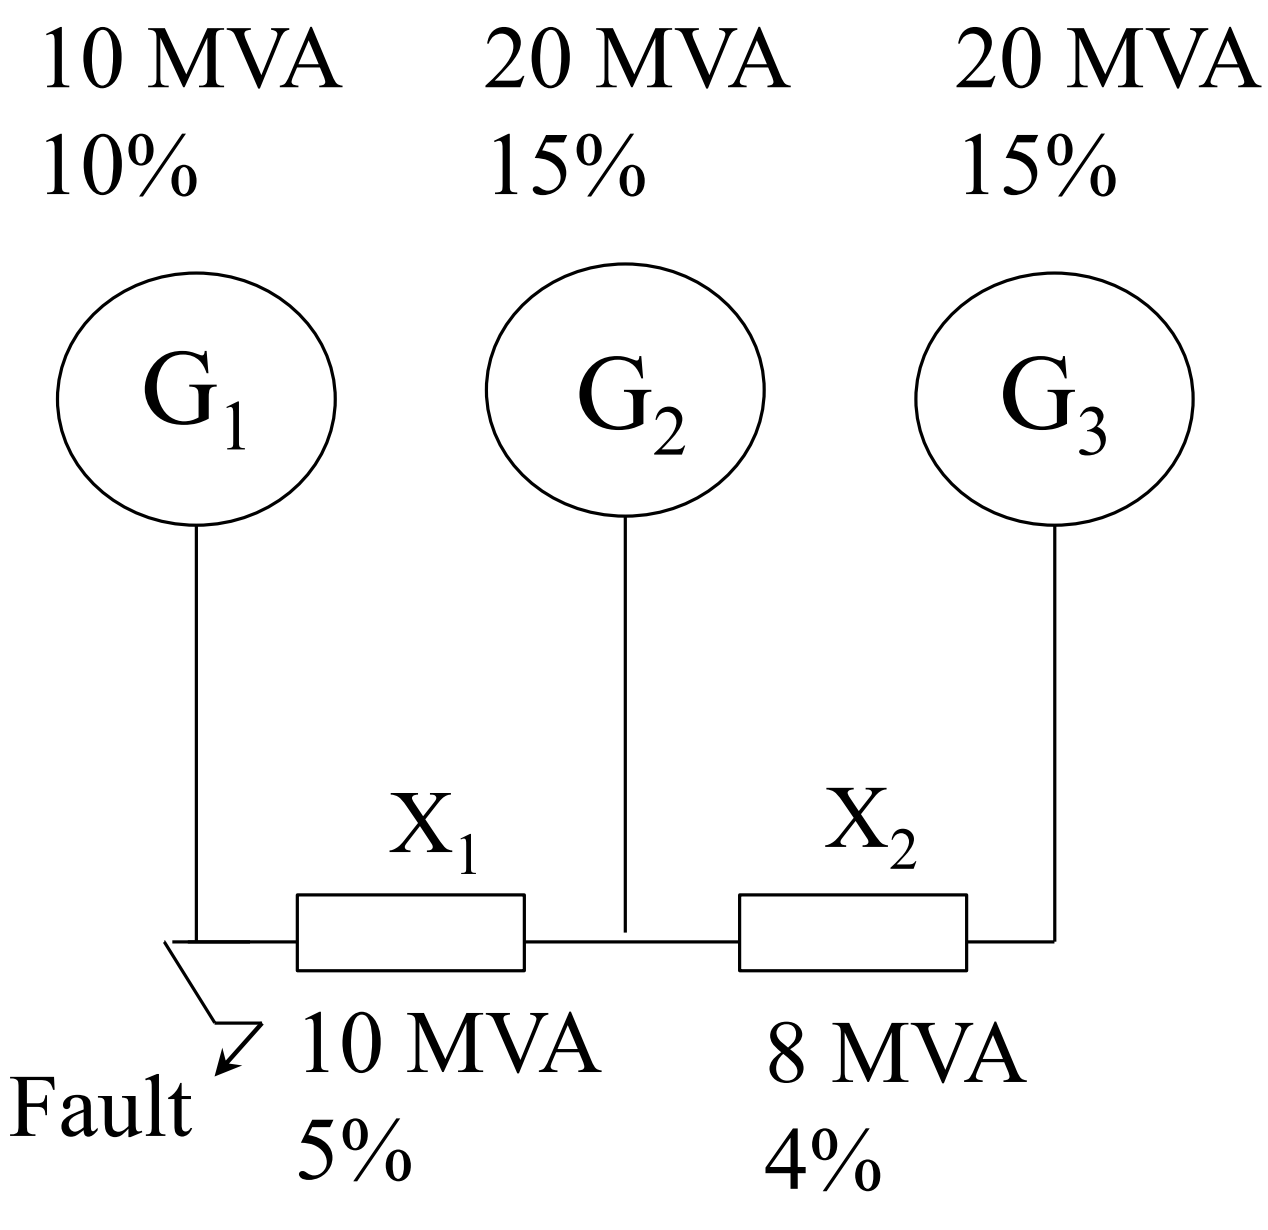
\includegraphics[width = 0.8\textwidth]{../img/figure17.png}
	\caption{Balanced three-phase fault.}
\end{figure}
An interconnected generator-reactor system is active and suddenly incurs a balanced three-phase short circuit at the Fault indicated. Using a \SI{50}{MVA} base then draw an impedance diagram and hence determine the Fault Level and Fault Current. It is an \SI{11}{kV} three phase system.
\subsection{Solution}
\begin{figure}[H]
	\centering
	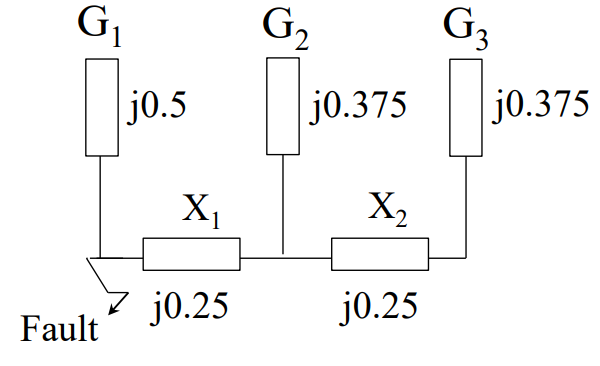
\includegraphics[width = 0.8\textwidth]{../img/figure18.png}
	\caption{Impedance diagram.}
\end{figure}
\begin{gather}
	X_{G1} = \frac{50}{10}\cdot 0.1 = \SI{0.5}{pu}\\
	X_{G2} = \frac{50}{20}\cdot 0.15 = \SI{0.375}{pu}\\
	X_{G3} = \frac{50}{20}\cdot 0.15 = \SI{0.375}{pu}\\
	X_1 = \frac{50}{10}\cdot 0.05 = \SI{0.25}{pu}\\
	X_1 = \frac{50}{8}\cdot 0.04 = \SI{0.25}{pu}
\end{gather}
\begin{figure}[H]
	\centering
	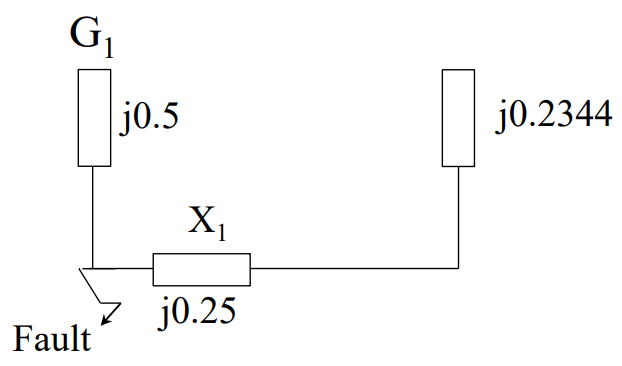
\includegraphics[width = 0.8\textwidth]{../img/figure19.png}
	\caption{Impedance diagram circuit reduced.}
\end{figure}
\begin{gather}
	\textrm{Per unit reactance} = \frac{0.5\left(0.2344 + 0.25\right)}{0.5 + \left(0.2344 + 0.25\right)} = j0.246\\
	\textrm{MVA Fault Level} = \frac{50\times 10^3}{0.246} = \SI{203.25}{MVA}\\
	\textrm{Fault current} = \frac{203.25 \times 10^6}{\sqrt{3}\times 11\times 10^3} = \SI{10668}{A}
\end{gather}
The MVA Fault Level provides information on the `power at the fault'. The Fault Current provides information on protection e.g. circuit breakers. This is known as the symmetrical fault current.
\subsection{Importance of MVA}
\begin{itemize}
	\item The short circuit capacity (SCC) at the busbar is the fault level of the busbar. The strength of a busbar (or the ability to maintain its voltage) is directly proportional to its SCC.
	\item An infinitely strong bus (or infinite bus bar) has an infinite SCC, with a zero equivalent impedance and will maintain its voltage under all conditions
	\item Magnitude of short circuit current is time dependent due to synchronous generators. It is initially at its largest value and decreasing to steady value. These higher fault levels tax circuit breakers (CB) adversely so that current limiting reactors are sometimes used
\end{itemize}
\subsection{Power system symmetrical faults}
\begin{itemize}
	\item In a power system, knowing the maximum MVA Fault Level and the Fault Current that could potentially flow into a zero impedance fault is necessary in order to rate switch gear correctly
	\item The MVA Fault Level defines the maximum MVA that is experience when a symmetrical fault event occurs. The fault level is usually expressed in MVA (or a corresponding per-unit value)
	\item The maximum fault current can be calculated using the MVA Fault Level and the nominal Voltage Rating at the fault location
\end{itemize}
\subsection{Conclusions}
\begin{itemize}
	\item The analysis show in this session has explained how impedance diagrams can be used for system analysis for `load flows' and `balanced faults'
	\item For larger or complex circuits then many more calculations are needed meaning computers are generally used to calculate load flows and faults
	\item Various computer programmes are available including MATLAB, Simulink Simpower Systems, PSCAD, ERACS, etc
\end{itemize}
\end{document}














\documentclass[class=report, crop=false, 12pt,a4paper]{standalone}
\usepackage{enumitem}
\usepackage{multicol}
\usepackage{graphicx}
\usepackage{float}
\usepackage{amsmath}
\usepackage{amssymb}
\usepackage{mathtools}
\usepackage{siunitx}
\usepackage{commath}
\usepackage{array}
\usepackage{natbib}
\usepackage[a4paper,width=150mm,top=25mm,bottom=25mm]{geometry}
\setlength{\parindent}{0pt}
\setlength{\parskip}{1em}
\raggedbottom
\begin{document}
\chapter{Faulted Networks}
\begin{itemize}
	\item Introducing the concept of unbalanced networks
	\item Using impedance diagrams for fault calculations
\end{itemize}
\subsection{Symmetrical faults recap}
In a power system the most significant fault that can occur is when all three-phases short together. This is a symmetrical or balanced fault. The MVA Fault Level defines the maximum MVA that the system is subjected to when a symmetrical fault event occurs. The fault level is usually expressed in MVA (or a corresponding per-unit value). The maximum fault current can be calculated using the MVA Fault Level and the nominal Voltage Rating at the fault location.
\section{Unbalanced faults}
\subsection{Types of `unbalanced faults'}
Unsymmetrical faults - currents and voltages are not balanced in each phase:
\begin{itemize}
	\item Single line to ground
	\item Line to line
	\item Double line to ground
	\item Single phase open circuit
	\item Dounle phase open circuit
\end{itemize}
For each short-circuit, the fault can be bolted (a zero impedance fault) or have a fault impedance known as Zf.
\begin{figure}[H]
	\centering
	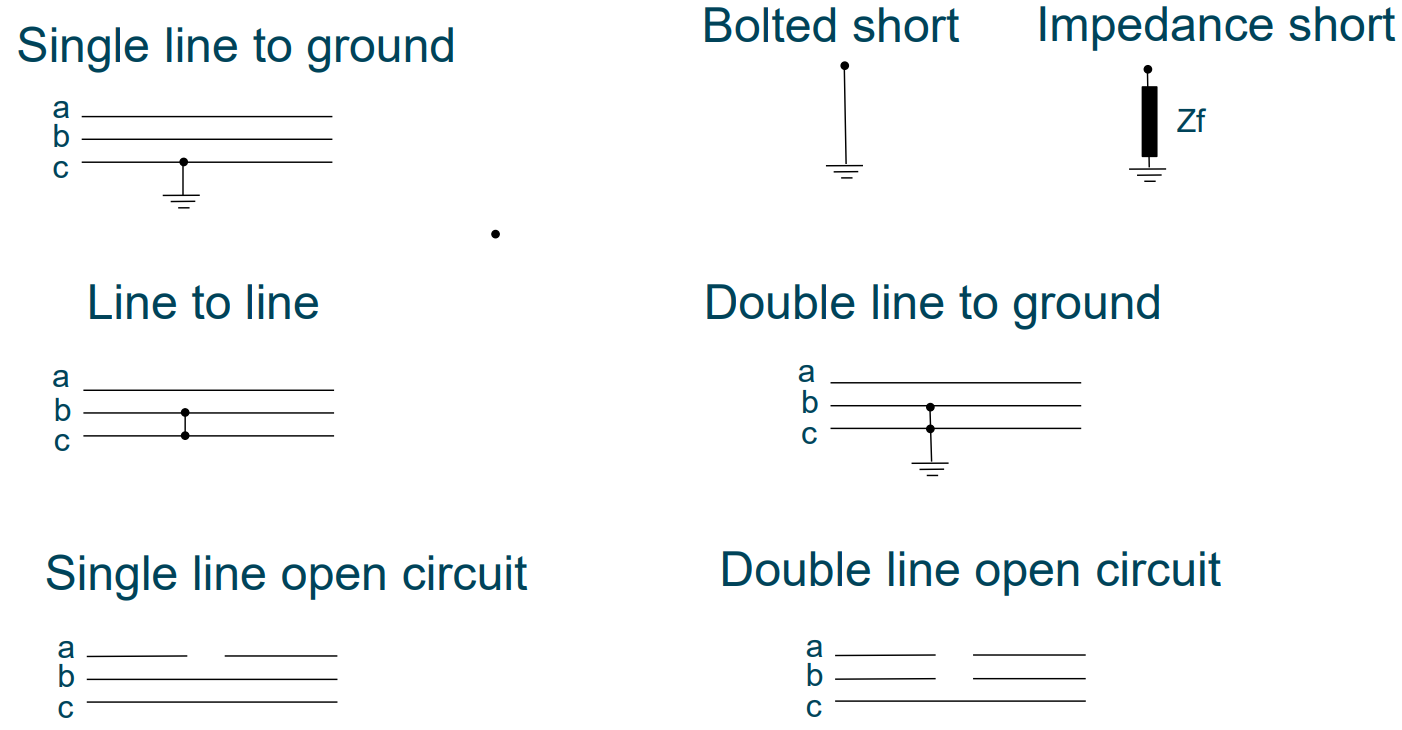
\includegraphics[width = \textwidth]{../img/figure20.png}
	\caption{Unsymmetrical/unbalanced faults.}
\end{figure}
\subsection{List of possible faults}
\begin{itemize}
	\item Three phase symmetrical fault L-L-L
	\item Three phase symmetrical fault L-L-L-G
	\item Line to line fault
	\item Double line to ground fault
	\item Single line to ground fault
	\item Single line open circuit
	\item Double line open circuit
\end{itemize}
The most common fault is the single line to ground fault. The worst fault is a three-phase to ground fault (L-L-L-G or L-L-L).
\begin{figure}[H]
	\centering
	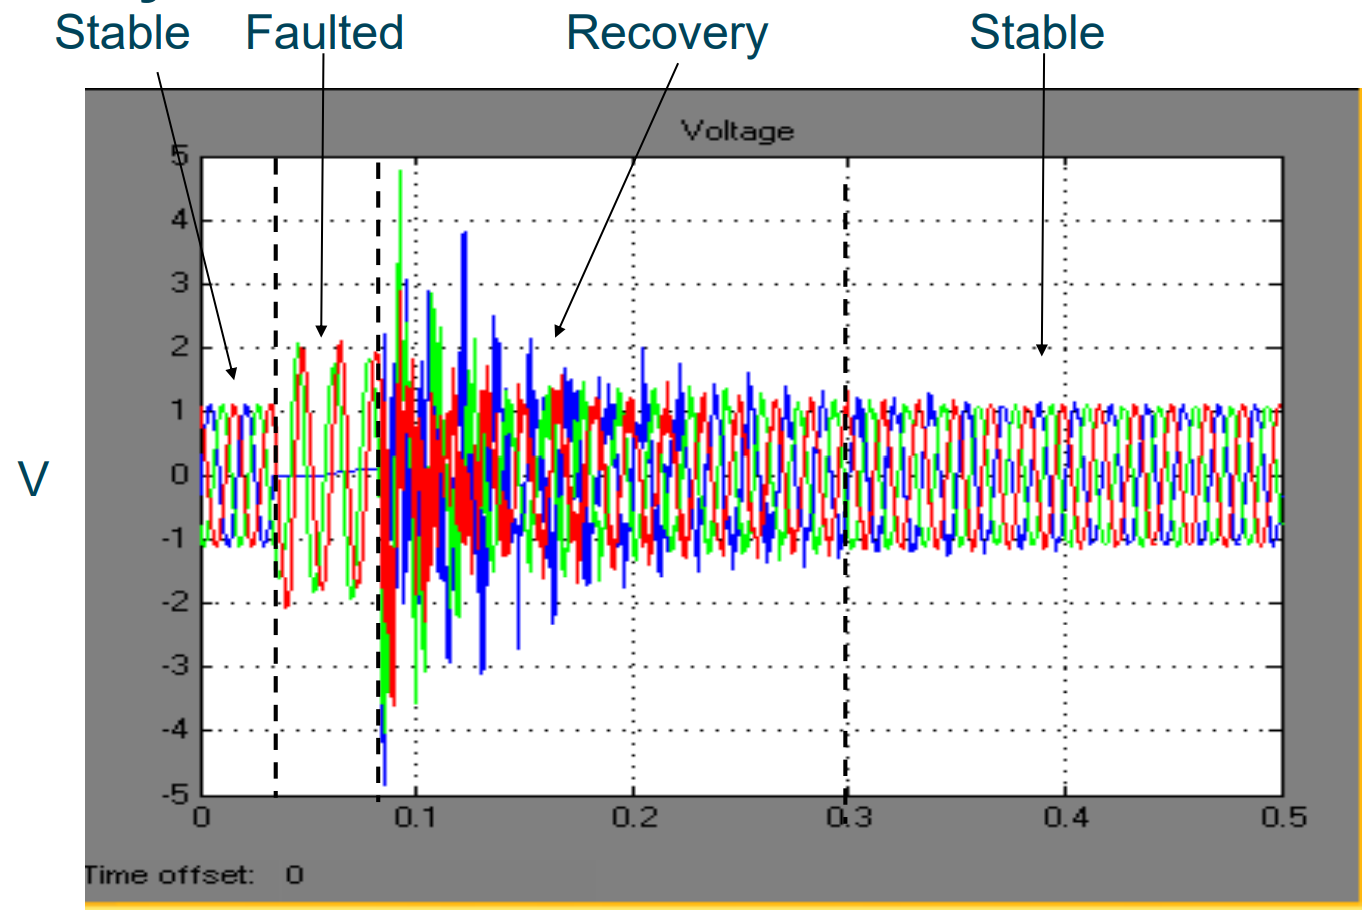
\includegraphics[width = \textwidth]{../img/figure21.png}
	\caption{Unsymmetrical/unbalanced fault graph.}
\end{figure}
We see the blue phase go to ground (0V) and the other two phases increase in voltage and are no longer \SI{120}{\degree} out of phase with each other. 
\subsection{Method of analysis}
Each phase is experiencing something different i.e. what is happening on one phase is not what is happening on the other. RMS voltages and currents are unbalanced.
\begin{gather}
	V_a \neq V_b \neq V_c \textrm{ nor } I_a \neq I_b \neq I_c
\end{gather}
The presumption that we used for symmetrical faults (the same equivalent circuit for each phase) is not valid in the unsymmetrical/unbalanced case. For the unbalanced case it is necessary to use a different method. We use `Fortescues's Theorem'.
\subsection{Fortescue's Theorem}
Fortescue's Theorem says:
\begin{quote}
	Three unbalanced phasors in a multi-phase electrical system can be resolved into a set of balanced phasors consisting of:
\end{quote}
\begin{itemize}
	\item Positive-sequence components
	\item Negative-sequence components
	\item Zero sequence components
\end{itemize}
\begin{align}
	V_{line} &= V_{positive} + V_{negative} + V_{zero}\\
	I_{line} &= I_{positive} + I_{negative} + I_{zero}
\end{align}
\subsection{Positive sequence components}
For a three-phase system there are three balanced phasors:
\begin{itemize}
	\item Equal in magnitude
	\item Displaced from each other by \SI{120}{\degree}
	\item Have phase sequence a-b-c
	\item Usually referred to as $V_{a1}$, $V_{b1}$, $V_{c1}$
\end{itemize}
\subsection{Negative sequence components}
For a three-phase system there are three balanced phasors:
\begin{itemize}
	\item Equal in magnitude
	\item Displaced from each other by \SI{120}{\degree}
	\item Have phase sequence a-c-b
	\item Usually referred to as $V_{a2}$, $V_{b2}$, $V_{c2}$
\end{itemize}
\subsection{Zero sequence components}
For a three-phase system there are three balanced phasors:
\begin{itemize}
	\item Equal in magnitude
	\item Zero phase displacement
	\item No phase sequence
	\item Usually referred to as $V_{a0}$, $V_{b0}$, $V_{c0}$
\end{itemize}
\begin{figure}[H]
	\centering
	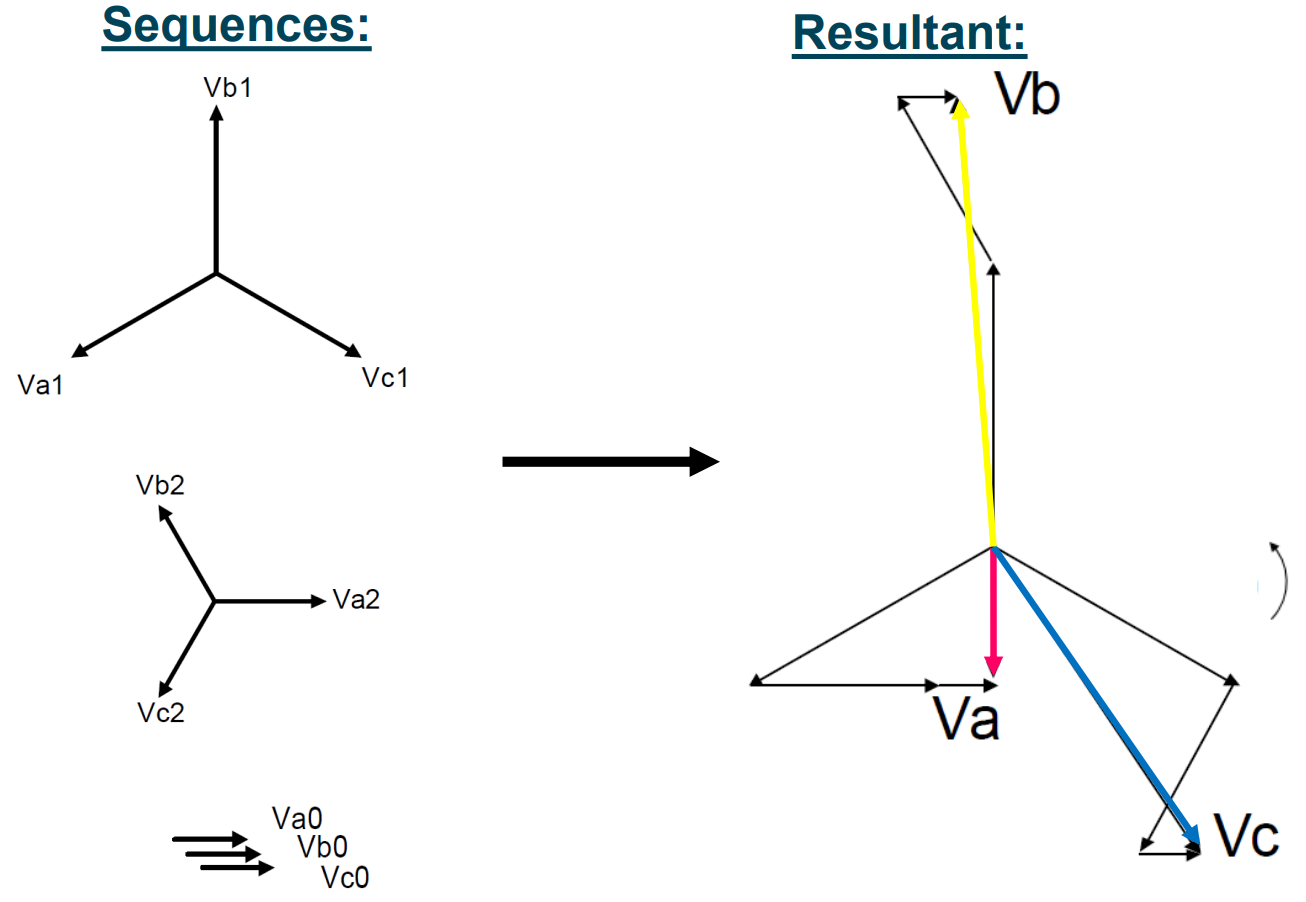
\includegraphics[width = \textwidth]{../img/figure22.png}
	\caption{Sequence components and phase relationship.}
\end{figure}
\begin{figure}[H]
	\centering
	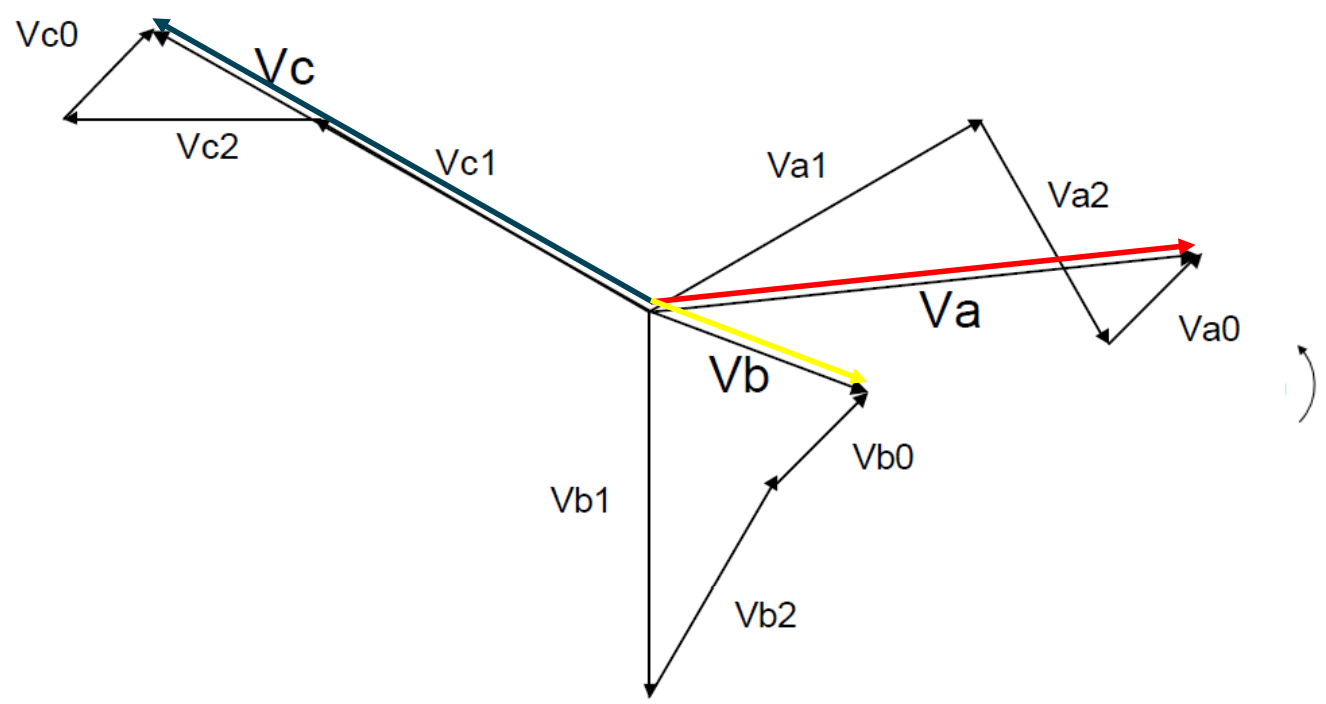
\includegraphics[width = \textwidth]{../img/figure23.png}
	\caption{Sequence components 2.}
\end{figure}
\subsection{Summing sequence components}
Original phasors are the sum of their components
\begin{align}
	V_a &= V_{a0} + V_{a1} + V_{a2}\\
	V_b &= V_{b0} + V_{b1} + V_{b2}\\
	V_c &= V_{c0} + V_{c1} + V_{c2}
\end{align}
Hence:
\begin{gather}
	\textrm{Line} = \sum \textrm{sequence components}
\end{gather}
In balanced/symmetrical networks in multi-phase systems then only positive sequence components are present.
\subsection{Note about grounding/earthing}
How a system is grounded has a major impact on fault current. Zero sequence current can only flow when the start point of the source is tied to ground / earth directly or via an impedance Ze. 
\begin{figure}[H]
	\centering
	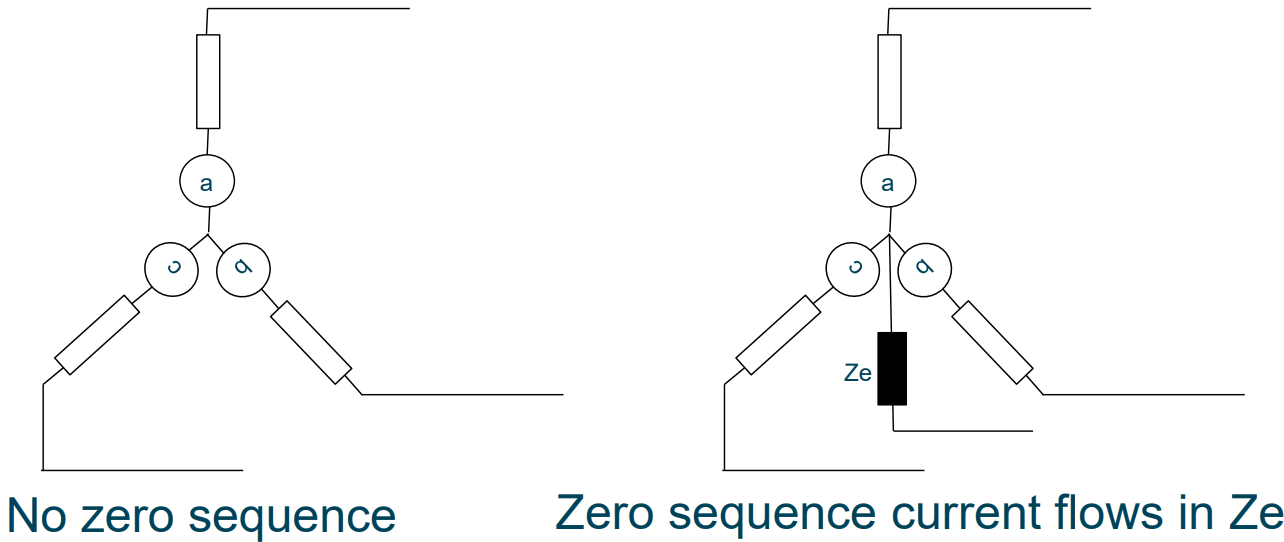
\includegraphics[width = \textwidth]{../img/figure24.png}
	\caption{Grounding/earthing.}
\end{figure}
We can see the virtual/floating star point on the sequence on the left. Normally, this is left floating on ship systems for example. The star point can be connected to ground (unusual for generators) or we can add an impedance to the star point connection. This is because the star point is not always 0V under a fault condition. Hence, by including an earth impedance, we can limit current flow.

Zero sequence current flows can only happen if we have a connection to ground. In floating star point connections, we cannot have zero sequence current flows.
\begin{figure}[H]
	\centering
	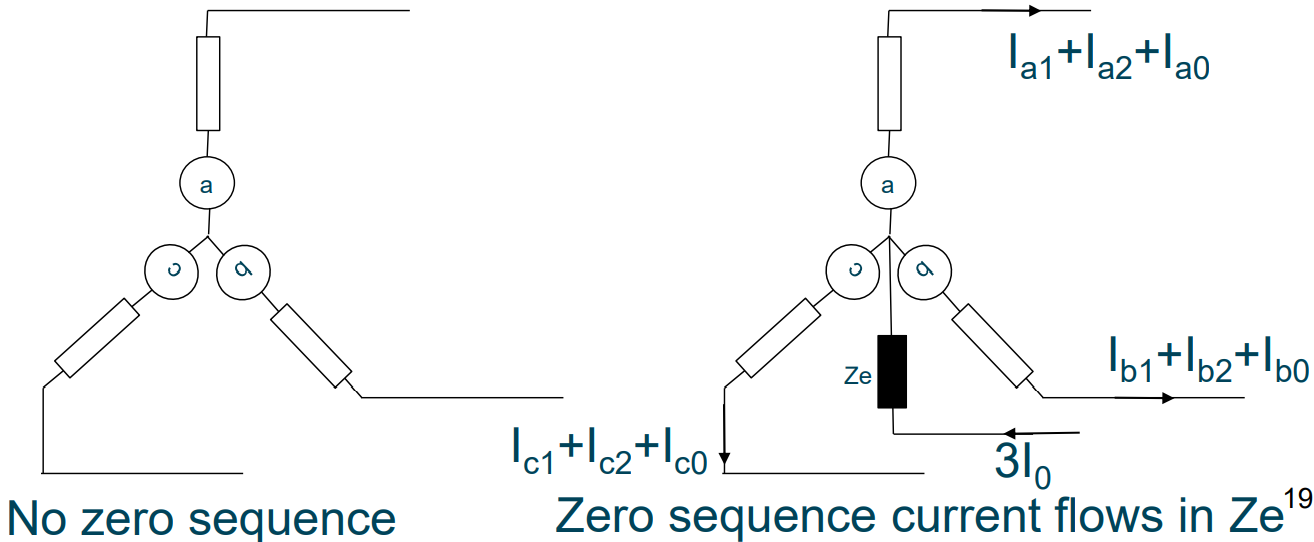
\includegraphics[width = \textwidth]{../img/figure25.png}
	\caption{Currents during grounded star point.}
\end{figure}
\begin{figure}[H]
	\centering
	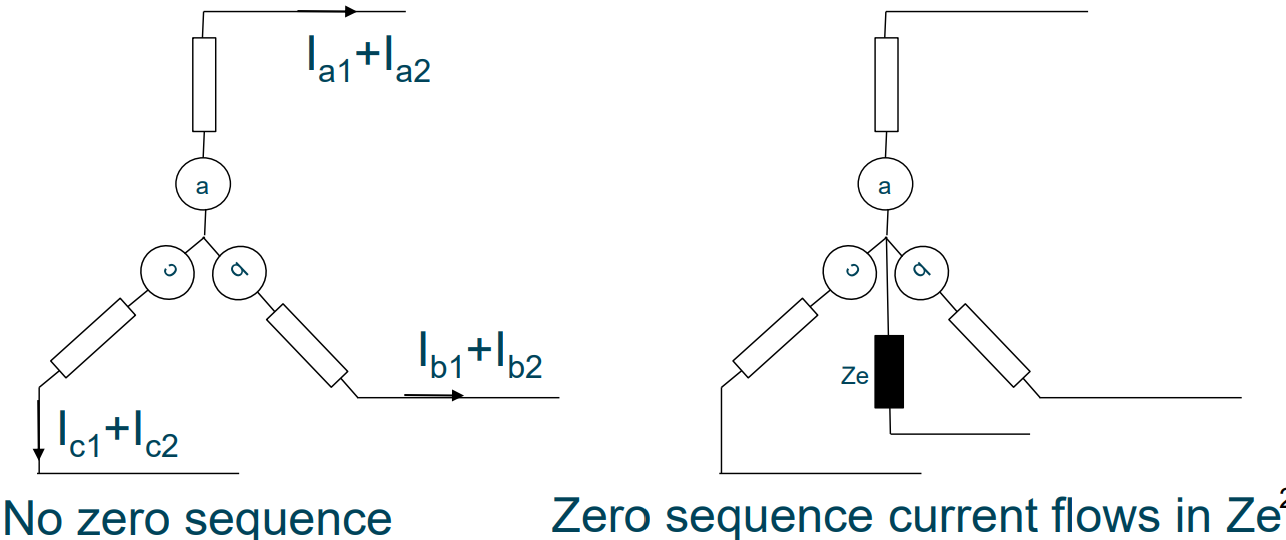
\includegraphics[width = \textwidth]{../img/figure26.png}
	\caption{Currents during floating star point.}
\end{figure}
\subsection{The operator `a'}
Let us define an operator that rotates a phasor by \SI{120}{\degree}:
\begin{gather}
	a = 1\angle \SI{120}{\degree} = (-0.5 + j 0.8666)
\end{gather}
\begin{figure}[H]
	\centering
	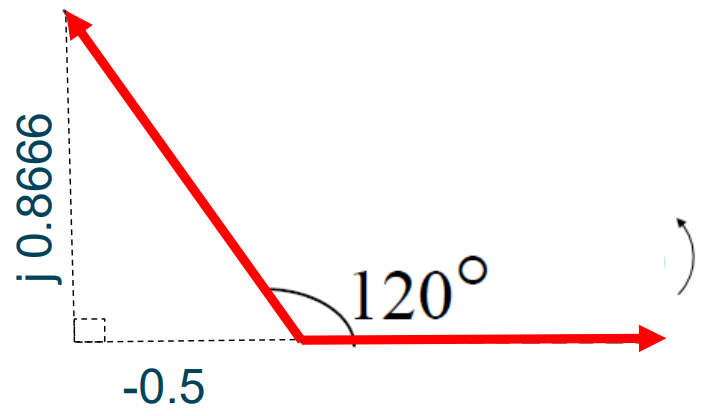
\includegraphics[width = 0.4\textwidth]{../img/figure27.png}
	\caption{`a' operator.}
\end{figure}
\subsection{Expressing phasors $a^2$ and $a^3$}
\begin{gather}
	a^2 = a \times a = \left(1 \angle \SI{240}{\degree}\right) = 1 \angle \SI{-120}{\degree}
\end{gather}
Similarly:
\begin{gather}
	a^3 = \left( 1 \angle \SI{360}{\degree}\right) = 1 \angle \SI{0}{\degree}
\end{gather}
Therefore:
\begin{align}
	a + a^2 + a^3 &= 0\\
	1 + a + a^2 &= 0
\end{align}
\begin{figure}[H]
	\centering
	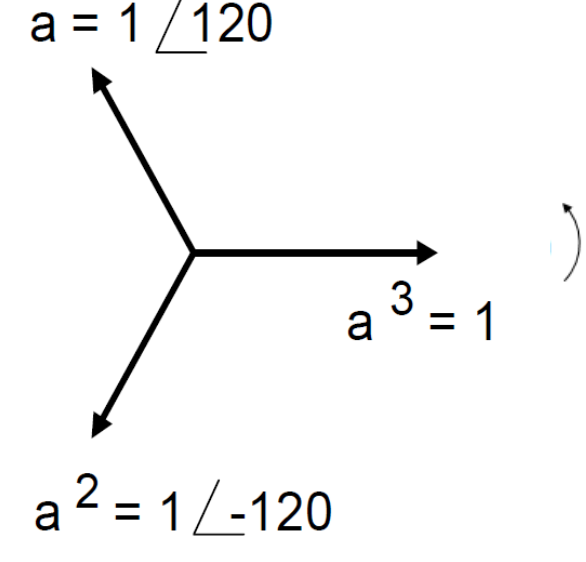
\includegraphics[width = 0.4\textwidth]{../img/figure28.png}
	\caption{`a' phasors.}
\end{figure}
The value of the star point changes with fault conditions.
\subsection{Representation using `a'}
Using the `a' operator then the positive sequence components can be written:
\begin{align}
	V_{a1} &= 1\\
	V_{b1} &= \left(1 \angle -\SI{120}{\degree}\right) = a^2 V_{a1}\\
	V_{c1} &= \left(1 \angle \SI{120}{\degree}\right) = a V_{a1}
\end{align}
In other words we have used the `a' operator to express $V_{b1}$ and $V_{c1}$ in terms of $V_{a1}$. Similarly for the negative sequence, we have:
\begin{align}
	V_{a2} &= 1\\
	V_{b2} &= \left(1 \angle \SI{120}{\degree}\right)V_{a2} = aV_{a2}\\
	V_{b2} &= \left(1 \angle \SI{-120}{\degree}\right)V_{a2} = a^2V_{a2}
\end{align}
In other words we have used the `a' operator to express $V_{b2}$ and $V_{c2}$ in terms of $V_{a2}$. For the zero sequence:
\begin{gather}
	V_{a0} = V_{b0} = V_{c0}
\end{gather}
No need for the operator `a' here as all zero sequence components are in phase!
\begin{figure}[H]
	\centering
	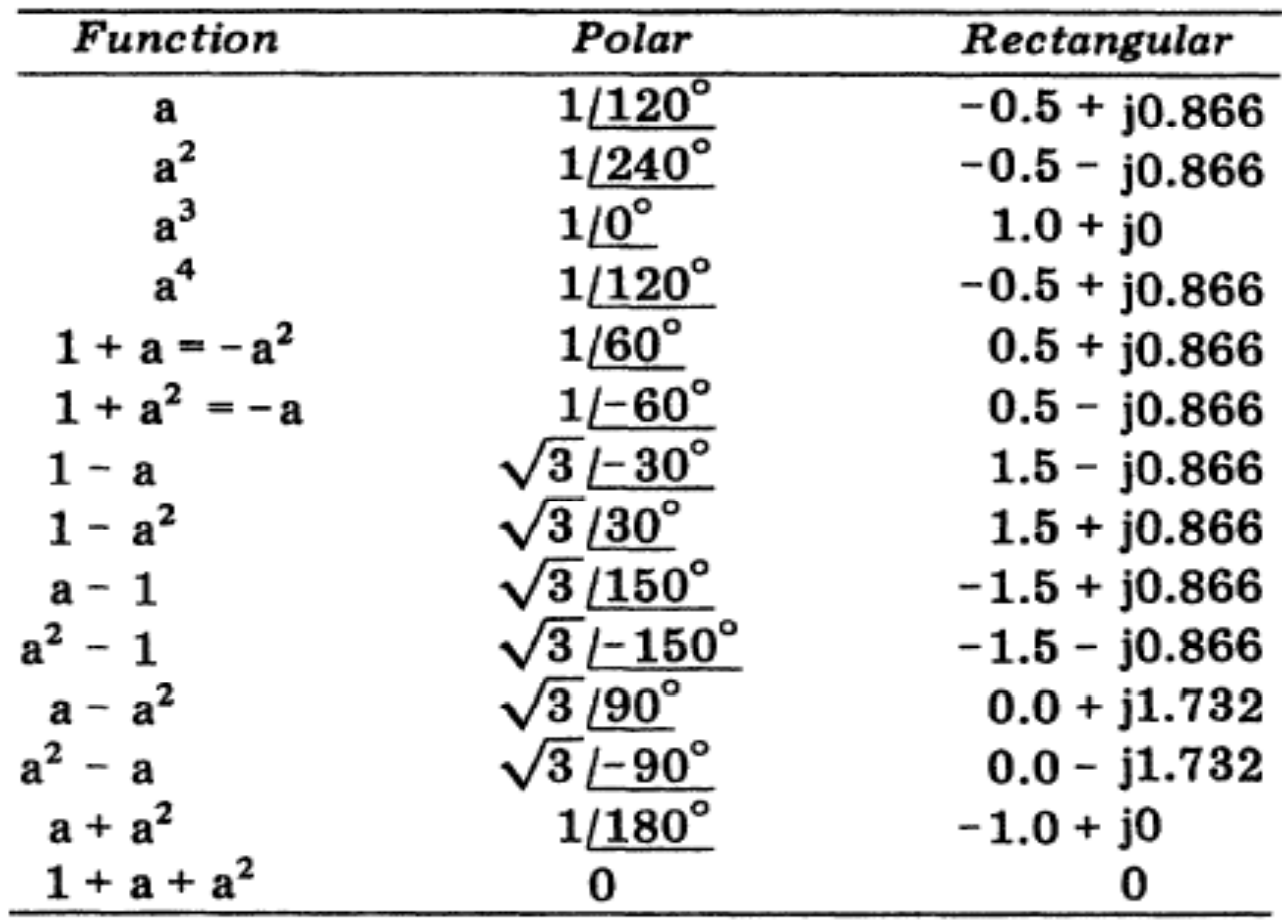
\includegraphics[width = \textwidth]{../img/figure29.png}
	\caption{List of `a' phasors.}
\end{figure}
\subsection{Representing all sequence components in terms of $V_{a}$ sequence components}
\begin{gather}
	\textrm{Line} = \sum \textrm{sequence components}\\
	V_a = V_{a0} + V_{a1} + V_{a2} = V_{a0} + V_{a1} + V_{a2}\\
	V_b = V_{b0} + V_{b1} + V_{b2} = V_{a0} + a^2 V_{a1} + aV_{a2}\\
	V_c = V_{c0} + V_{c1} + V_{c2} = V_{a0} + aV_{a1} + a^2V_{a2}
\end{gather}
\begin{figure}[H]
	\centering
	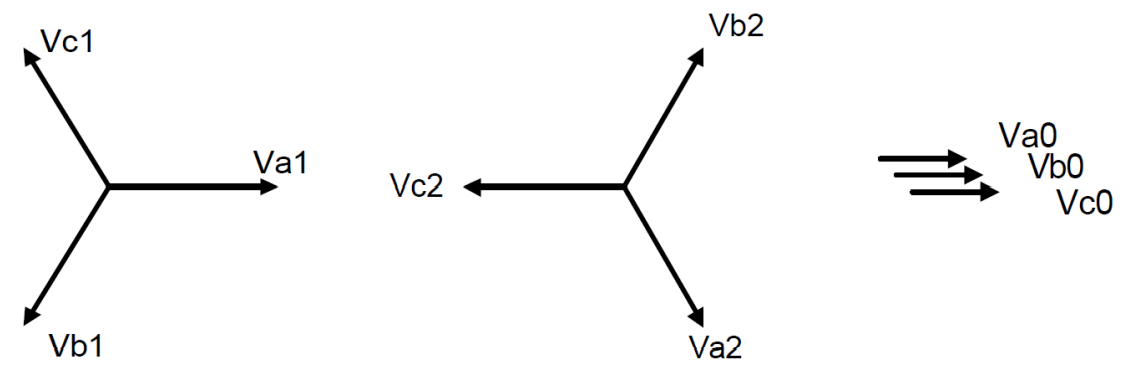
\includegraphics[width = \textwidth]{../img/figure30.png}
	\caption{Phase voltages expressed in terms of $V_{a}$.}
\end{figure}
\subsection{`a' matrix}
\begin{gather}
	\textrm{Line} = \sum \textrm{sequence components}\\
	\begin{bmatrix}
		V_a\\
		V_b\\
		V_c
	\end{bmatrix} = \begin{bmatrix}
		1 & 1 & 1\\
		1 & a^2 & a\\
		1 & a & a^2
	\end{bmatrix}\begin{bmatrix}
		V_{a0}\\
		V_{a1}\\
		V_{a2}
	\end{bmatrix}
\end{gather}
\subsection{Inverse `a' matrix}
The sequences may be described by the `inverse a matrix' and phasors:
\begin{gather}
	\begin{bmatrix}
		V_{a0}\\
		V_{a1}\\
		b_{a2}
	\end{bmatrix} = \frac{1}{3}\begin{bmatrix}
		1 & 1 & 1\\
		1 & a & a^2\\
		1 & a^2 & a
	\end{bmatrix}\begin{bmatrix}
		V_a\\
		V_b\\
		V_c
	\end{bmatrix}
\end{gather}
Where:
\begin{gather}
	A^{-1} = \frac{1}{3}\begin{bmatrix}
		1 & 1 & 1\\
		1 & a & a^2\\
		1 & a^2 & a
	\end{bmatrix}
\end{gather}
\subsection{Example}
A three-phase star connected load is connected across a three-phase balanced supply system. Obtain a set of equations relating the symmetrical components of a line and its phase voltages. Assuming:
\begin{gather}
	V_{ab} = V_a - V_b
\end{gather}
We will do this for one line voltage\dots

Zero sequence. Since:
\begin{gather}
	V_{ab} + V_{bc} + V_{ca} = 0
\end{gather}
then
\begin{gather}
	V_{ab0} + V_{bc0} + V_{ca0} = 0
\end{gather}
In other words there is no change in the zero sequence relationships. Assume balance

Positive sequence:
Choosing $V_{ab}$ then:
\begin{align}
	V_{ab1} &= \frac{1}{3}\left(V_{ab} + aV_{bc} + a^2 V_{ca}\right) \textrm{ from inverse `a' matrix}\\
	&= \frac{1}{3}\left[\left(V_a - V_b\right) + a\left(V_b- V_c\right)+a^2 \left(V_c - V_a\right)\right]\\
	\dots\\
	&= \frac{1}{3}\left[\left(1-a^2\right)\left(V_a + aV_b + a^2 V_c\right)\right]\\
	&= \left(1-a^2\right)V_{a1} \textrm{ from table}\\
	&= \sqrt{3} V_{a1} e^{j30} \textrm{ using exp form}
\end{align}
Negative sequence:
\begin{align}
	V_{ab2} &= \frac{1}{3}\left(V_{ab} + a^2V_{bc} + a V_{ca}\right) \textrm{ from inverse `a' matrix}\\
	&= \frac{1}{3}\left[\left(V_a - V_b\right) + a^2\left(V_b- V_c\right)+a \left(V_c - V_a\right)\right]\\
	\dots\\
	&= \frac{1}{3}\left[\left(1-a\right)\left(V_a + a^2V_b + a V_c\right)\right]\\
	&= \left(1-a\right)V_{a2} \textrm{ from table}\\
	&= \sqrt{3} V_{a2} e^{-j30} \textrm{ using exp form}
\end{align}
\subsection{Sequence components and faults}
\begin{itemize}
	\item This lecture started by considering unsymmetrical faults
	\item The lecture has introduced the method of sequence components and has provided a method analysis of unsymmetrical faults based on Fortescue's theorem
	\item Manipulation of the voltages and currents using the `a' matrix is an important step since this provides the analytical means to analyse unsymmetrical faults from sequence, phase and line perspectives
	\item In the next lecture we will look at unsymmetrical faults by applying this methodology
\end{itemize}
\subsection{Conclusions}
\begin{itemize}
	\item The analysis shown in this session has explained the system analysis methods for `unbalanced faults'
	\item The introuction to the `a' matrix which will be used for relationships between phase and line values and also introuced sequence components
	\item Appreciate the need for positive, negative and zero sequence impedances of different components that make up a power system
\end{itemize}
\end{document}














\chapter{Full Fault Analysis}
\section{Unbalanced impedance}
\subsection{Impedance and sequence components}
We have established that in a three-phase unbalanced network there are line and phase voltages and currents that deviate in their relationships from the balanced case. Furthermore, any unbalance can be described as a set of sequence components consisting positive, negative and zero sequence phasors. Now considering impedances in unbalanced networks then we need to ensure that we understand:
\begin{itemize}
	\item How to change between star and delta arrangements
	\item Appreciate how sequence impedance is calculated
\end{itemize}
\subsection{Unbalanced star and delta equivalence}
$Z_{delta} = 3\cdot Z_{star}$ for all three phases when the loads in the three-phase system were balanced. This was helpful when looking at symmetrical faults since we normally convert delta connections into star connections and consider an impedance diagram as representing one phase. When loads are unbalanced then we need to consider each phase independently because they are subjected to different voltages, currents and impedances. Consider the two circuits below. The star and delta equivalence must result in the same line voltages and currents. In other words the impedance between any two impedances must be equivalent.
\begin{figure}[H]
	\centering
	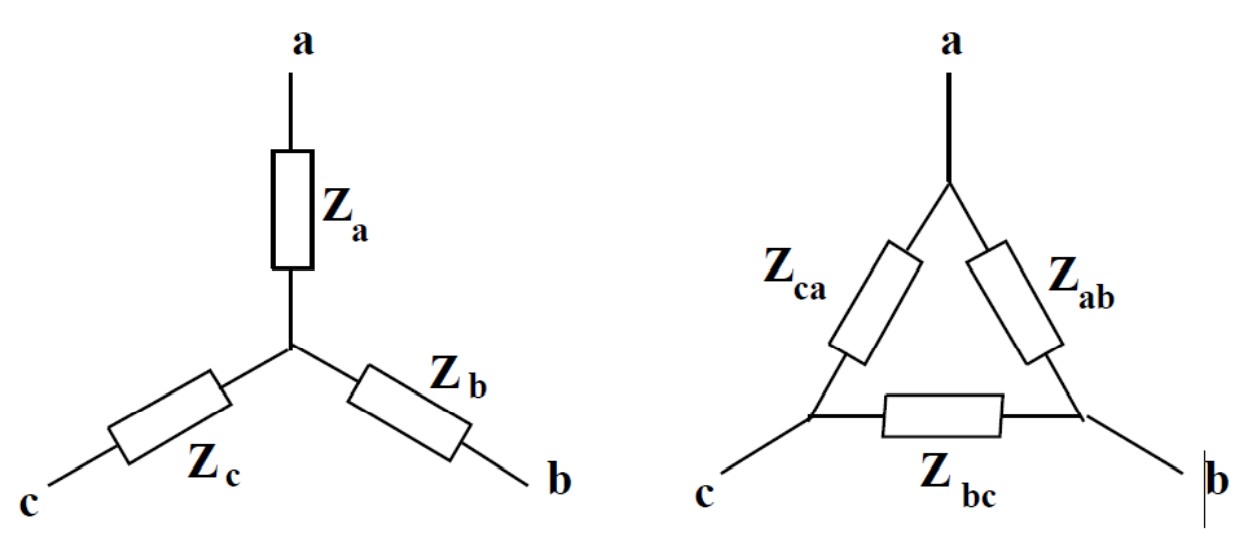
\includegraphics[width = \textwidth]{./img/figure31.png}
	\caption{Star and delta arrangements.}
\end{figure}
For example considering phase a and phase b, the impedance equivalence must be:
\begin{gather}
	Z_a + Z_b = Z_{ab} // \left(Z_{ca}+Z_{bc}\right) \textrm{ similarly,}\\
	Z_b + Z_c = Z_{bc} // \left(Z_{ab}+Z_{ca}\right)\\
	Z_c + Z_a = Z_{ca} // \left(Z_{bc}+Z_{ab}\right)
\end{gather}
By manipulation and substitution then it is possible to derive the following relationships:
\begin{gather}
	Z_{ab} = \frac{Z_aZ_b + Z_bZ_c+Z_cZ_a}{Z_c}\\
	Z_{bc} = \frac{Z_aZ_b + Z_bZ_c+Z_cZ_a}{Z_a}\\
	Z_{ca} = \frac{Z_aZ_b + Z_bZ_c+Z_cZ_a}{Z_b}
\end{gather}
and
\begin{gather}
	Z_a = \frac{Z_{ab}Z_{ca}}{Z_{ab}+Z_{bc}+Z_{ca}}\\
	Z_b = \frac{Z_{ab}Z_{bc}}{Z_{ab}+Z_{bc}+Z_{ca}}\\
	Z_b = \frac{Z_{bc}Z_{ca}}{Z_{ab}+Z_{bc}+Z_{ca}}
\end{gather}
These relationships are needed when considering impedance in unbalanced loads.
\subsection{Good practice}
In many fault calculations it is handy to convert delta impedances into star impedances because:
\begin{itemize}
	\item It ensures that all balanced arrangements are related to ground or virtual group (floating star point)
	\item When calculating faults then it is apparent that such calculations are made for one phase and then `phase shifted' to determine impact on other phases. Having everything as a star arrangement (mathematically and circuit wise) assits in ensuring that right values are obtained.
\end{itemize}
\section{Impedance of sequences}
There are positive, negative and zero phase sequence components: In voltage these are represented by $V_0$, $V_1$ and $V_2$. In current these are represented by $I_0$, $I_1$ and $I_2$.
\subsection{Sequence components and impedance}
Since $V=IZ$, it follows if there are sequence components in both voltage and current then there must be a sequence impedance too:
\begin{itemize}
	\item $V_1 = I_1 Z_1$ where $Z_1$ is the positive sequence impedance
	\item $V_2 = I_2 Z_2$ where $Z_2$ is the negative sequence impedance
	\item $V_0 = I_0 Z_0$ where $Z_0$ is the zero sequence impedance
\end{itemize}
\subsection{The importance of sequence impedance}
The impedance of a network is important for calculating currents for an applied voltage. Remembering earlier work on balanced networks, we established that the impedance limited the fault current i.e. the further from the source you were the greater the impedance. the lower the fault current. Now considering the sequence components, it is apparent that the sequence impedances $Z_0$, $Z_1$, $Z_2$ will limit sequence currents $I_0$, $I_1$, $I_2$ for the applied sequence voltages $V_0$, $V_1$, $V_2$.
\subsection{Network elements}
Different network equipment exhibit different sequence impedances:
\begin{itemize}
	\item Typically, transmission lines and cables have one impedance value for positive and negative sequence, but an entirely different impedance value for zero sequence
	\item Typically, rotating machines e.g. generators and mots have different impedance values for all three sequences
	\item Typically, transformers positive, negative and zero sequence components depend upon connection by positive and negative are often the same value
\end{itemize}
Appreciating these different impedances is important for accurate calculation of unsymmetrical faults.
\subsection{Transmission lines and distribution cables}
Power cables and transmission linse are used to carry power from the source to the load. Typically (over short distances) they can be represented as resistance and inductance. The inductance is comprised of its own self-inductance and mutual inductance between each line or cable.
\subsection{Transmission line analysis}
In a three-phase system interconnected between a three-phase generator and three-phase load the lines/cables usually run close to each so there is always mutual inductance and self-inductance of the lines.
\begin{figure}[H]
	\centering
	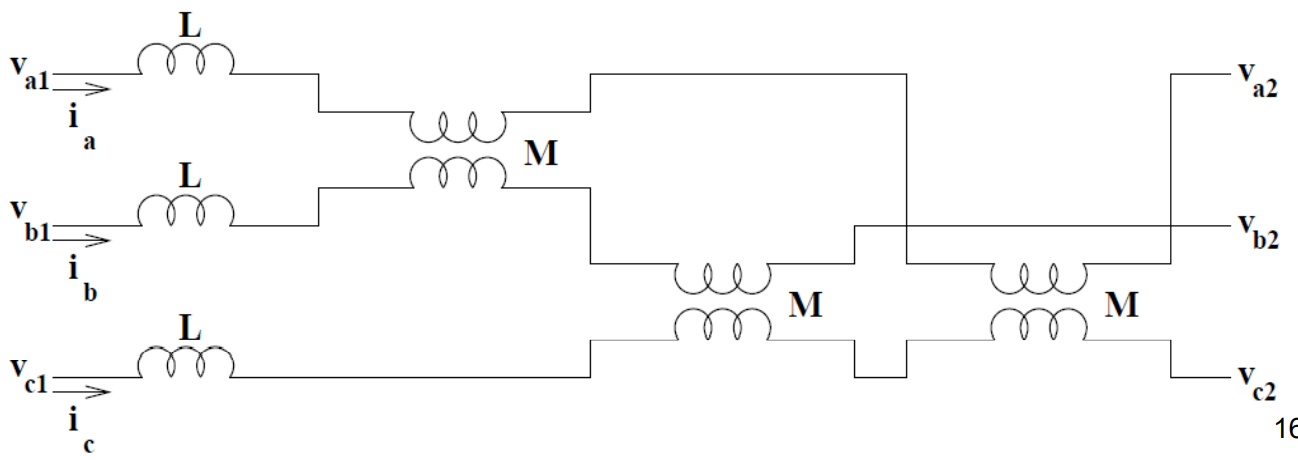
\includegraphics[width = \textwidth]{./img/figure32.png}
	\caption{Trasmission line mutual inductance and self-inductance.}
\end{figure}
\subsection{Transmission line representation}
Hence, we can write the relationship $(V = XI)$:
\begin{gather}
	\begin{pmatrix}
		V_a \\
		V_b \\
		V_c
	\end{pmatrix} = j \omega \begin{pmatrix}
		L_a    & M_{ab} & M_{ac} \\
		M_{ba} & L_b    & M_{bc} \\
		M_{ca} & M_{cb} & L_c
	\end{pmatrix}\begin{pmatrix}
		I_a \\
		I_b \\
		I_c
	\end{pmatrix}
\end{gather}
It is reasonable to say that the line and mutual inductances are the same for each transmission line or cable under steady-state balanced conditions. This is not necessarily the case for transient or unbalanced case.
\subsection{Transmission sequence representation}
Bringing in the relationship between phase and sequence components we have (ignoring 1/3):
\begin{gather}
	I_{sequence} = \left[A\right]^{-1} \cdot I_{phase}\\
	V_{sequence} = \left[A\right]^{-1} \cdot V_{phase}
\end{gather}
Hence:
\begin{gather}
	\begin{pmatrix}
		1   & 1   & 1 \\
		a^2 & a   & 1 \\
		a   & a^2 & 1
	\end{pmatrix}\begin{pmatrix}
		V_1 \\
		V_2 \\
		V_3
	\end{pmatrix} = j\omega\begin{pmatrix}
		L_a    & M_{ab} & M_{ac} \\
		M_{ba} & L_b    & M_{bc} \\
		M_{ca} & M_{cb} & L_c
	\end{pmatrix}\cdot\begin{pmatrix}
		1   & 1   & 1 \\
		a^2 & a   & 1 \\
		a   & a^2 & 1
	\end{pmatrix}\begin{pmatrix}
		I_a \\
		I_b \\
		I_c
	\end{pmatrix}\\
	\left[A\right] \left[V_{sequence}\right] = j\omega \left[LM\right]\cdot \left[A\right]\left[I_{sequence}\right]
\end{gather}
\subsection{Transmission line representation}
Hence by transformation we obtain:
\begin{gather}
	\left[V_{sequence}\right] = j\omega\left[A\right]\cdot \left[LM\right]\cdot\left[A\right]^{-1}\left[I_{sequence}\right]
\end{gather}
The part ($\left[A\right]\cdot \left[LM\right]\cdot\left[A\right]^{-1}$) provides the inductance sequence relationship for the transmission line or distribution cable. Resolving gives:
\begin{gather}
	\begin{pmatrix}
		L-M & 0    & 0    \\
		0   & L- M & 0    \\
		0   & 0    & L+2M
	\end{pmatrix}
\end{gather}
The relationship between sequence components becomes:
\begin{gather}
	\begin{pmatrix}
		V_1 \\
		V_2 \\
		V_3
	\end{pmatrix} = j \omega \begin{pmatrix}
		L-M & 0    & 0    \\
		0   & L- M & 0    \\
		0   & 0    & L+2M
	\end{pmatrix} \begin{pmatrix}
		I_a \\
		I_b \\
		I_c
	\end{pmatrix}
\end{gather}
The sequence component relationships become:
\begin{gather}
	V_1 = j\omega \left(L - M\right)I_1\\
	V_2 = j\omega \left(L - M\right)I_2\\
	V_0 = j\omega \left(L - M\right)I_0
\end{gather}
The positive, negative and zero sequence reactances of the balanced transmission line are then:
\begin{gather}
	Z_1 = Z_2 = j\omega \left(L-M\right) \\
	Z_0 = j\omega \left(L+2M\right)
\end{gather}
\begin{figure}[H]
	\centering
	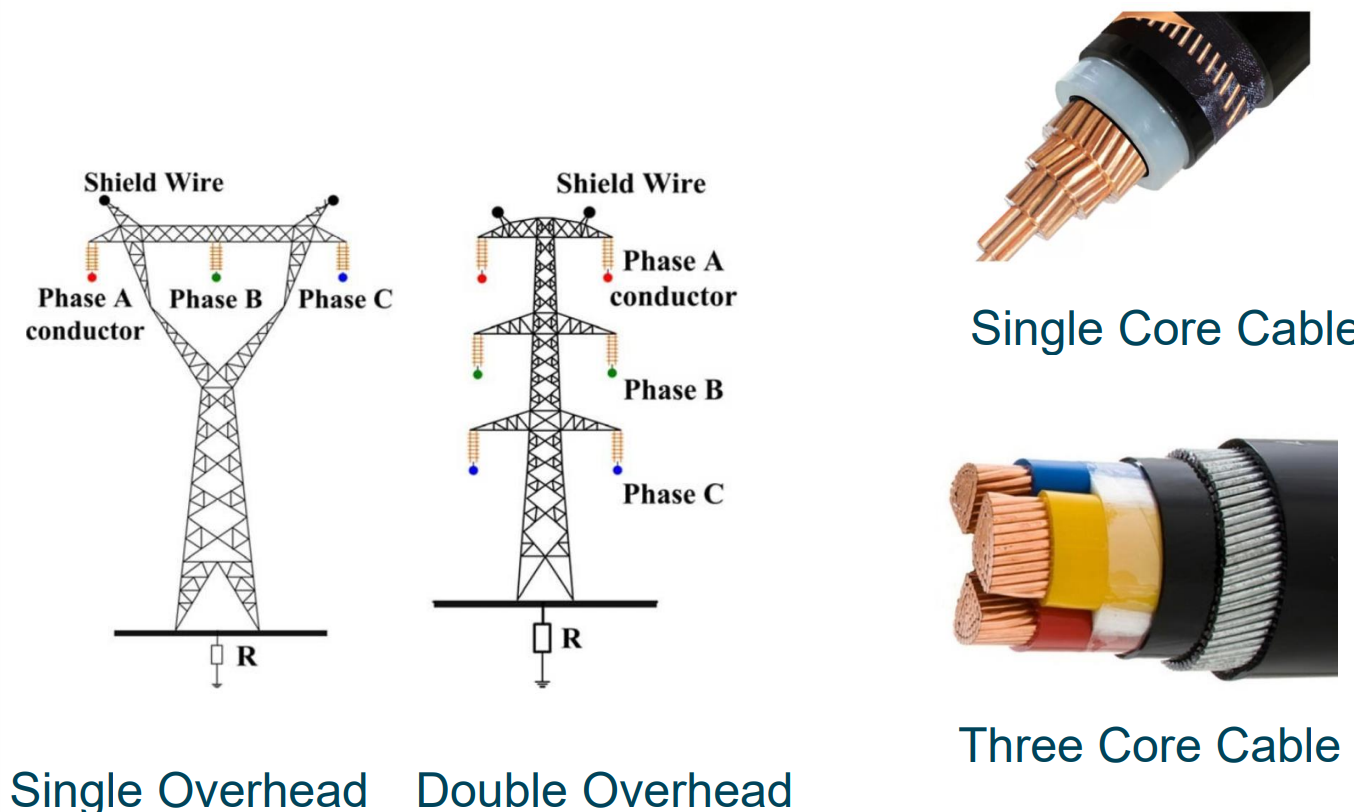
\includegraphics[width = \textwidth]{./img/figure33.png}
	\caption{Transmission line and cable arrangements.}
\end{figure}
\subsection{Lines and cables}
The positive and negative sequence impedances are normally balanced i.e. $Z_1 = Z_2$. The zero sequence impedance depends upon the nature of the return path through the earth. Typical relative values of $Z_0$ during faults are

Overhead:
\begin{itemize}
	\item For a single-circuit arrangement ($Z_0/Z_1$) = 3.5
	\item For a double-circuit arrangement ($Z_0/Z_1$) = 5.5
\end{itemize}
Cable arrangements:
\begin{itemize}
	\item For a single-core arrangement ($Z_0/Z_1$) = 1.25
	\item For a three-core arrangement ($Z_0/Z_1$) = 4
\end{itemize}
\subsection{Synchronous machines (generators)}
The positive sequence reactance $Z_1$ is the value used under balanced operation due to positive sequence currents flowing in the windings of the machine in steady-state and transient. The negative sequence reactance $Z_2$ is due to negative sequence currents which give rise to fluxes in the air gap of the machine that rotate in the opposite direction during unbalance. $Z_2$ is different to $Z_1$ in most designs. The zero sequence reactance $Z_0$ depends upon the nature of the connection of the star point. Zero sequence currents will not flow when the star point is floating but will flow when there is.
\subsection{Neutral connection}
The symmetrical components are independent with the voltage-current relationships:
\begin{gather}
	V_1 = ZI_1\\
	V_2 = ZI_2\\
	V_0 = \left(Z + 3Z_g\right)I_0
\end{gather}
In many generators that are tied to ground at the star point will have additional impedance separately added to reduce the level of zero sequence currents.
\begin{figure}[H]
	\centering
	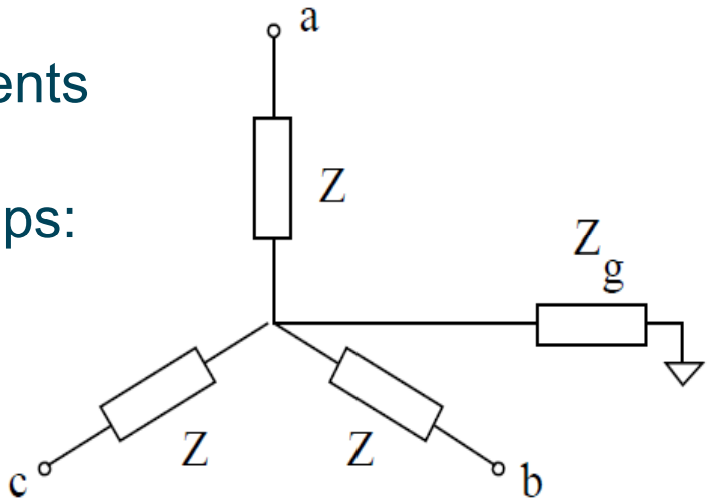
\includegraphics[width = 0.6\textwidth]{./img/figure34.png}
	\caption{Grounded star arrangement.}
\end{figure}
\subsection{Typical values of sequence impedances for synchronous generators}
\begin{table}
	\centering
	\begin{tabular}{@{}llll@{}}
		\toprule
		Type of machine                           & +ve sequence  & -ve sequence  & zero sequence \\
		\midrule
		\SI{440}{V} \SI{50}{\hertz} \SI{1}{MVA}   & \SI{0.16}{pu} & \SI{0.11}{pu} & \SI{0.05}{pu} \\
		\SI{11}{kV} \SI{50}{\hertz} \SI{75}{MVA}  & \SI{0.18}{pu} & \SI{0.14}{pu} & \SI{0.07}{pu} \\
		\SI{16}{kV} \SI{50}{\hertz} \SI{275}{MVA} & \SI{0.21}{pu} & \SI{0.18}{pu} & \SI{0.08}{pu} \\
		\SI{22}{kV} \SI{50}{\hertz} \SI{575}{MVA} & \SI{0.28}{pu} & \SI{0.21}{pu} & \SI{0.12}{pu} \\
		\bottomrule
	\end{tabular}
	\caption{Table to show typical value of sequence impedances for synchronous generators}
\end{table}
Manufacturers will test their machines to obtain the relevant data/ The value of the sequence components may differ from country to country, manufacturer to manufacturer.
\subsection{Transformers}
The positive and negative sequence sequence impedances are the normal values obtained from the per-phase equivalent circuit. ($Z_1 = Z_2$). The zero sequence components depend upon the connection of the windings. Zero sequence currents in the windings on one side of the transformer must produce the corresponding ampere-turns in the other. In delta windings the zero-sequence currents circulate through the three-phase windings but do not leave the transformer.
\section{Unbalanced faults}
\subsection{Fortescue's symmetrical component process}
Symmetrical components are used extensively for fault study calculations. in these calculations the positive, negative and zero-sequence impedance networks are either given by the manufacturer or are calculated by the user using base voltages and base power for the system of interest. Each of the sequence networks are then connected together to calculate fault currents and voltages depending upon the type of fault. Standard circuit arrangements have been derived in this course to keep variation reasonable.
\begin{figure}[H]
	\centering
	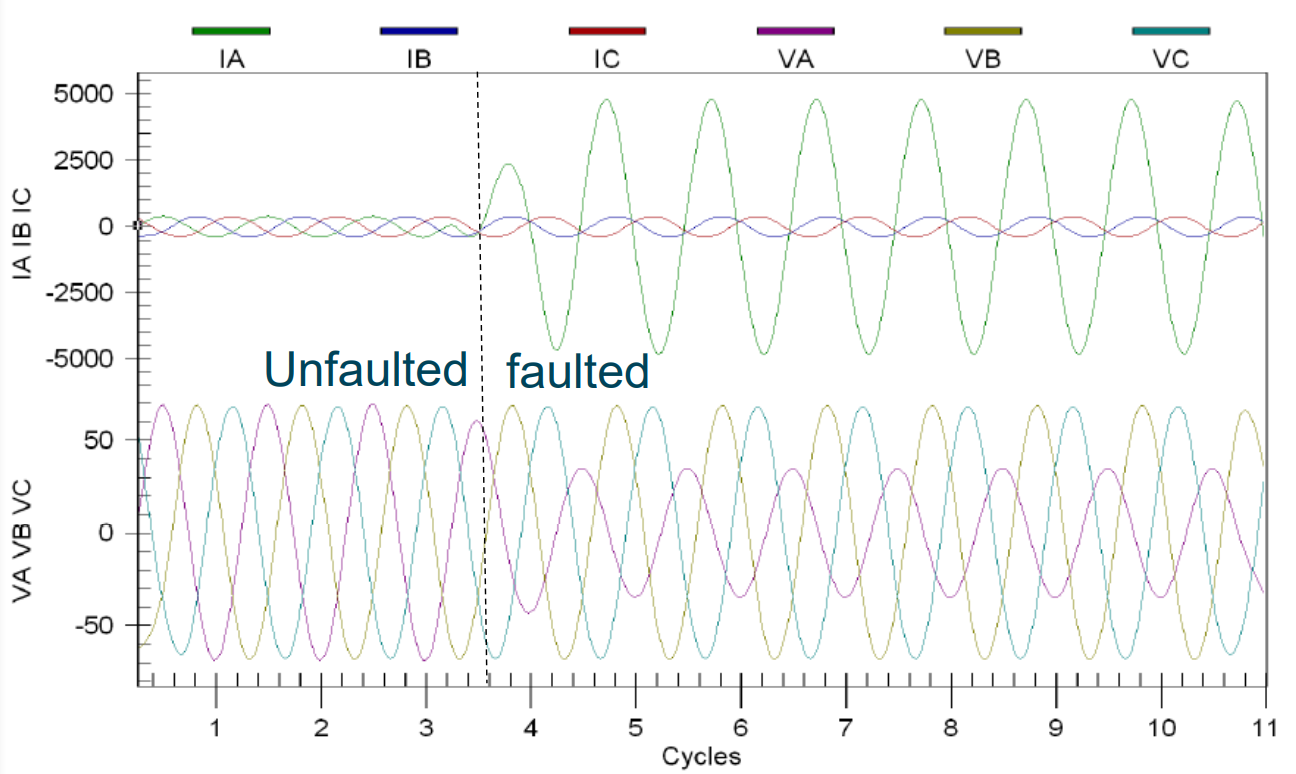
\includegraphics[width = \textwidth]{./img/figure35.png}
	\caption{Line to ground fault.}
\end{figure}
\subsection{Standard fault sequence connections - single line to ground}
\begin{figure}[H]
	\centering
	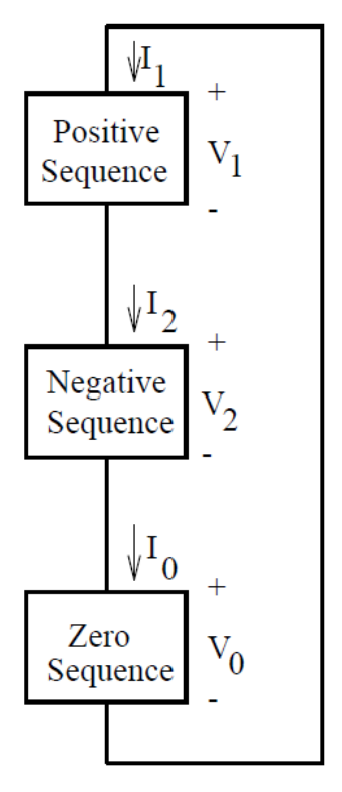
\includegraphics[width = 0.3 \textwidth]{./img/figure36.png}
	\caption{Single line to ground connection.}
\end{figure}
Assumptions:
\begin{itemize}
	\item $V_a = 0$; $I_a$ = very large value (faulted line)
	\item $I_b = 0$ (small in comparision to fault current)
	\item $I_c = 0$ (small in comparision to fault current)
\end{itemize}
Hence for phae voltage `a' we can say:
\begin{gather}
	V_0 + V_1 + V_2 = 0
\end{gather}
And for the current we can say:
\begin{gather}
	I_0 + I_1 + I_2 = \frac{1}{3}I_a
\end{gather}
Together, these two expressions describe the sequence network connection.
\subsection{Standard fault sequence connections - line to line}
\begin{figure}[H]
	\centering
	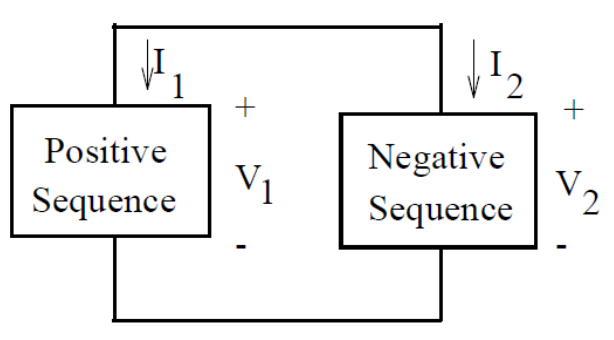
\includegraphics[width = 0.4 \textwidth]{./img/figure37.png}
	\caption{Line to line connection.}
\end{figure}
Assumptions. If the fault occurs between phase b and c then we can say:
\begin{itemize}
	\item $V_b = V_c$
	\item $I_b = -I_c$
	\item $I_a = 0$ (since it is small in comparison with the fault current)
\end{itemize}
Hence, we can use the phase sequence relationships to say:
\begin{gather}
	V_1 = V_2 \textrm{ and also } I_a = I_1 + I_2 \textrm{ since } I_0 = 0
\end{gather}
\subsection{Standard fault sequence connections - double line to ground}
\begin{figure}[H]
	\centering
	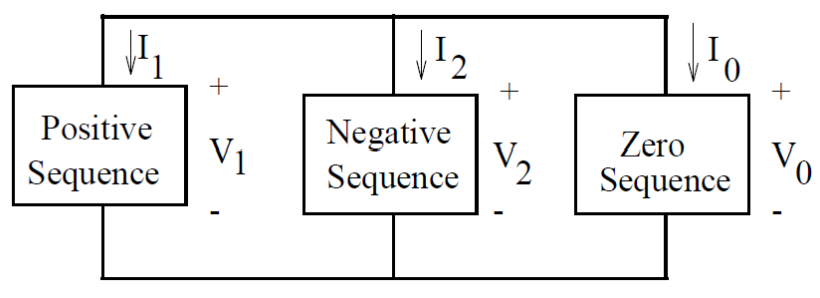
\includegraphics[width = 0.7\textwidth]{./img/figure38.png}
	\caption{Double line to ground connection.}
\end{figure}
Assumptions. If the fault involves phases b and c to ground then we can say:
\begin{itemize}
	\item $I_a = 0$ (small in comparison to fault current)
	\item $V_b = 0$ (faulted line)
	\item $V_c = 0$ (faulted line)
\end{itemize}
Hence using phase-sequence relationships we can further say that:
\begin{gather}
	V_0 + V_1 + V_2 = 0\\
	I_a = I_0 + I_1 + I_2 = 0
\end{gather}
\section{A full fault analysis study}
\subsection{Breaker sizing method (most common approach)}
One of the main purposes of circuit breakers is to arrest large currents that flow when there is a fault. Breaker sizing is achieved by understanding currents flowing under both symmetrical and non-symmetrical fault conditions (to be calculated). Calculations are carried out using symmetrical components i.e. positive, negative and zero sequence. Only one phae needs to be considered \dots but all fault types need to be calculated.
\subsection{Breaker sizing example}
Determine the maximum current through the breaker B due to a fault at the location X. Calculate all three types of unbalanced fult and the balanced fault currents.
\begin{itemize}
	\item System base: voltage \SI{138}{kV} (\SI{1}{pu}), Power \SI{100}{MVA} (\SI{1}{pu})
	\item Transformer $T_1$ leakage reactance j0.1 pu
	\item Transformer $T_2$ leakage reactance j0.1 pu
	\item Line L1: positive and negative sequence reactance j0.05 pu, zero sequence reactance j0.1 pu
	\item Line L2: positive and negative sequence reactance j0.02 pu, zero sequence reactance j0.1 pu
\end{itemize}
\begin{figure}[H]
	\centering
	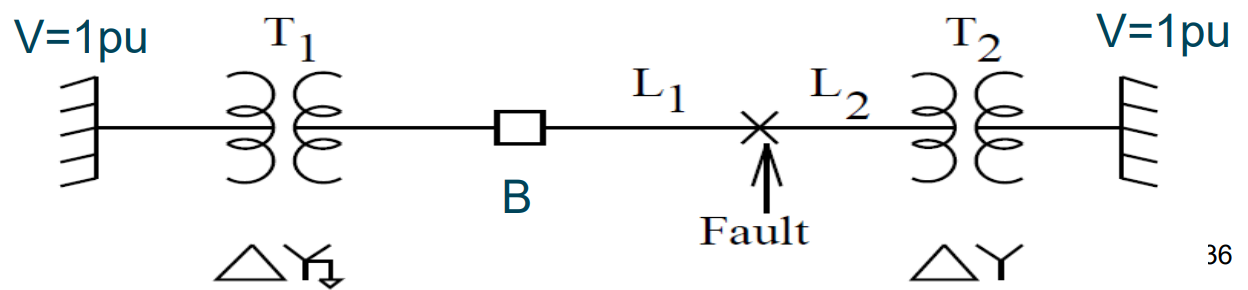
\includegraphics[width = \textwidth]{./img/figure39.png}
	\caption{Breaker sizing example.}
\end{figure}
\subsection{Sequence component arrangement}
\begin{figure}[H]
	\centering
	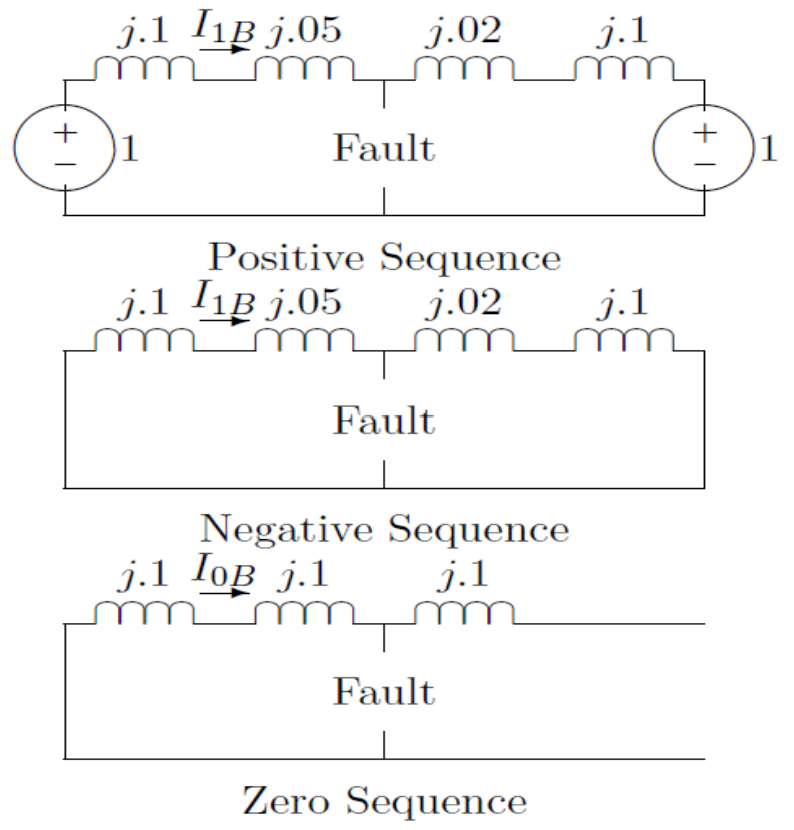
\includegraphics[width = 0.5\textwidth]{./img/figure40.png}
	\caption{Sequence component arrangement.}
\end{figure}
The sequence networks are exactly like what we would expect to have drawn for equivalent single phase networks. A positive, negative and zero sequence arrangmenet has been shown for one phase. Only the positive sequence network has sources, because the infinite bus supplies only positive sequence voltage. The zero sequence network is open at the right hand side because of the delta-wye transformer connection.
\subsection{Symmetrical fault current}
For a symmetrical (three-phase) fault, only the positive sequence network is involved. The fault shorts the network at its position, so that the current is:
\begin{gather}
	I_1 = \frac{1}{j0.15} - j6.67 \textrm{ per unit from LHS}\\
	(I_1 = \frac{1}{j0.12} - j8.33 \textrm{ per unit from RHS})
\end{gather}
\begin{figure}[H]
	\centering
	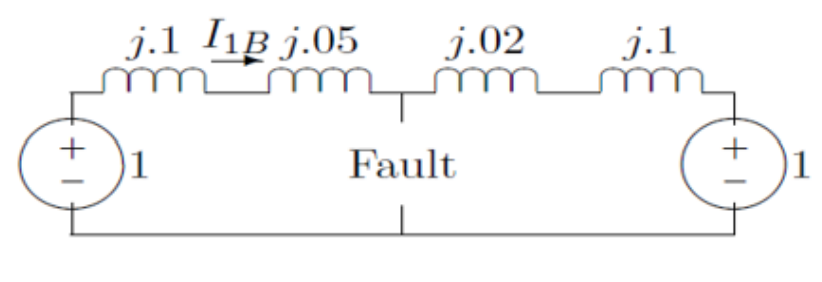
\includegraphics[width = 0.8\textwidth]{./img/figure41.png}
	\caption{Positive sequence impedance in symmetrical fault.}
\end{figure}
\subsection{Single line to ground fault}
\begin{figure}[H]
	\centering
	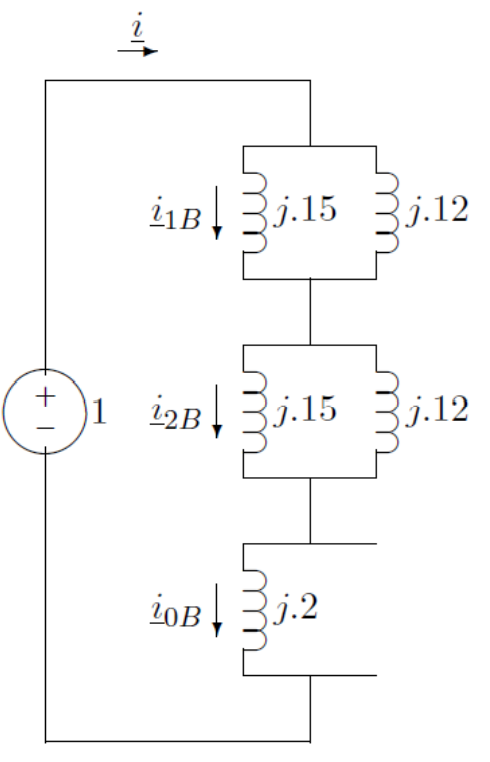
\includegraphics[width = 0.4\textwidth]{./img/figure42.png}
	\caption{Positive sequence impedance in symmetrical fault.}
\end{figure}
The three networks are in series and the situation is as shown with the total current given by:
\begin{gather}
	\underline{i} = \frac{1}{2 \times \left(j0.15 || j0.12\right) + j0.2} = -j3.0
\end{gather}
The sequence currents are:
\begin{align}
	\underline{i}_{1B} & = \underline{i}_{2B}                               \\
	                   & = \underline{i} \times \frac{j0.12}{j0.12 + j0.15} \\
	                   & = -j1.33
	\underline{i}_{0B} & = \underline{i}                                    \\
	                   & = -j3.0
\end{align}
\subsection{Singe line to ground fault}
Having calculated the sequence currents, the phase currents can be reconstructed:
\begin{align}
	\underline{i}_a & = \underline{i}_{1B} + \underline{i}_{2B} + \underline{i}_{0B}     \\
	\underline{i}_b & = \underline{a^2i}_{1B} + \underline{ai}_{2B} + \underline{i}_{0B} \\
	\underline{i}_c & = \underline{ai}_{1B} + \underline{a^2i}_{2B} + \underline{i}_{0B}
\end{align}
Hence:
\begin{align}
	\underline{i}_a & = -j5.66\, \textrm{pu} \\
	\underline{i}_b & = -j1.67\, \textrm{pu} \\
	\underline{i}_c & = -j1.67\, \textrm{pu}
\end{align}
\subsection{Double line to ground fault}
\begin{figure}[H]
	\centering
	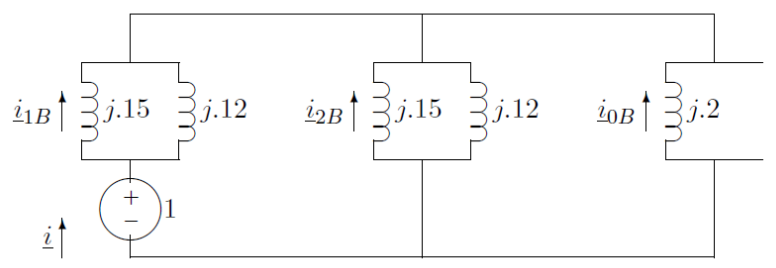
\includegraphics[width = \textwidth]{./img/figure43.png}
	\caption{Double line-ground fault configuration.}
\end{figure}
For the double line-ground fault, the networks are in parallel.
\begin{align}
	\underline{i}      & = \frac{1}{j\left(0.15||0.12\right)+ j \left(0.15||0.12||0.2\right)} \\
	                   & = -j8.57                                                             \\
	\underline{i}_{1B} & = \underline{i} \times \frac{j0.12}{j0.12 + j0.15}                   \\
	                   & = -j3.81                                                             \\
	\underline{i}_{2B} & = -\underline{i} \times \frac{j0.12 ||j0.2}{j0.12||j0.2 + j0.15}     \\
	                   & = j2.86                                                              \\
	\underline{i}_{0B} & = \underline{i}\times \frac{j0.12||j0.15}{j0.2 + j0.12||j0.15}       \\
	                   & = j2.14
\end{align}
Having calculated the sequence currents, the phase currents can be reconstructed:
\begin{align}
	\underline{i}_a & = j1.19                                                                                                                                                          \\
	\underline{i}_b & = \underline{i}_{0B} - \frac{1}{2}\left(\underline{i}_{1B} + \underline{i}_{2B}\right)-\frac{\sqrt{3}}{2}j\left(\underline{i}_{1B} - \underline{i}_{2B}\right)   \\
	                & = j2.67 - 5.87                                                                                                                                                   \\
	\underline{i}_c & = \underline{i}_{0B} - \frac{1}{2}\left(\underline{i}_{1B}+\underline{i}_{2B}\right) + \frac{\sqrt{3}}{2} j \left(\underline{i}_{1B} - \underline{i}_{2B}\right) \\
	                & = j2.67 + 5.87
\end{align}
Hence:
\begin{align}
	\left| \underline{i}_{a}\right| & = 1.19\, \textrm{pu} \\
	\left| \underline{i}_{b}\right| & = 6.43\, \textrm{pu} \\
	\left| \underline{i}_{c}\right| & = 6.43\, \textrm{pu}
\end{align}
\subsection{Line to line fault}
Having calculated the sequence currents, the phase currents can be reconstructed:
\begin{align}
	\underline{i}_a & = 0                                                                                                                                       \\
	\underline{i}_b & = -\frac{1}{2}\left(\underline{i}_{1B}+ \underline{i}_{2B}\right) - j\frac{\sqrt{3}}{2}\left(\underline{i}_{1B}-\underline{i}_{2B}\right)
\end{align}
Hence:
\begin{align}
	\left|\underline{i}_{b}\right| & = 5.77\, \textrm{pu} \\
	\left|\underline{i}_{c}\right| & = 5.77\, \textrm{pu}
\end{align}
There are only two networks at play - positive and negative sequence.
\begin{figure}[H]
	\centering
	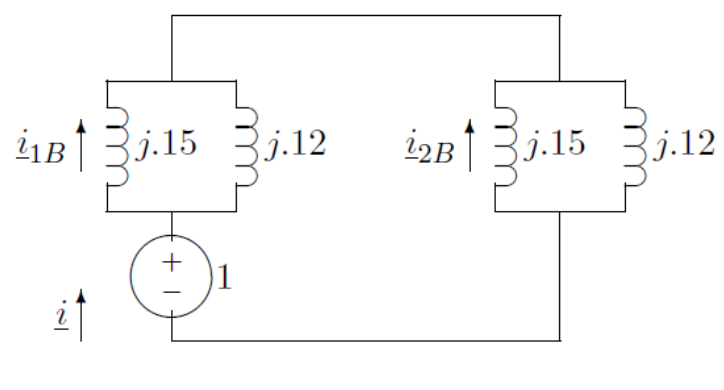
\includegraphics[width = 0.5\textwidth]{./img/figure44.png}
	\caption{Line to line fault configuration.}
\end{figure}
\subsection{Conversion to ampere ratings}
Having calculated the fault currents then the values in per unit can be expressed as amperes. The value of $I_B$ is:
\begin{gather}
	I_B = \frac{P_B}{\sqrt{3}V_{Bl-l}} = \SI{418.8}{A}
\end{gather}
Hence the fault currents are calculated as being:
\begin{table}
	\centering
	\begin{tabular}{@{}llll@{}}
		\toprule
		                                       & Phase A & Phase B & Phase C \\
		\midrule
		Three-phase fault                      & 2791    & 2791    & 2791    \\
		Single line-ground, $\phi_a$           & 2368    & 699     & 699     \\
		Double line-ground, $\phi_b$, $\phi_c$ & 498     & 2690    & 2690    \\
		Line-line, $\phi_b$, $\phi_c$          & 0       & 2414    & 2414    \\
		\bottomrule
	\end{tabular}
	\caption{Table to show fault currents.}
\end{table}
The worst fault is the balanced three-phase fault.
\subsection{Practical sizing of breakers}
Key information needed for sizing a circuit breaker include:
\begin{itemize}
	\item Voltage rating
	\item Normal current rating
	\item MVA fault level
	\item Fault current levels
	\item Withstand voltage levels
\end{itemize}
There are three main types of circuit breakers: Air, vacuum and SF6.
\subsection{Conclusions}
\begin{itemize}
	\item Appreciated the need for positive, negative and zero sequence impedances of different components to make up a power system
	\item Introduced the concept of positive, negative and zero sequence impedance. Examined this at a component level
	\item A system analysis method has been applied for `unbalanced faults' in a transmission system and fault current table produced
\end{itemize}
\chapter{Network Analysis}
\section{Network analysis}
\subsection{Electrical networks}
Note that the system interconnects in a complex pattern allowing for multiple current paths. How to determine voltage and current flows?
\begin{figure}[H]
	\centering
	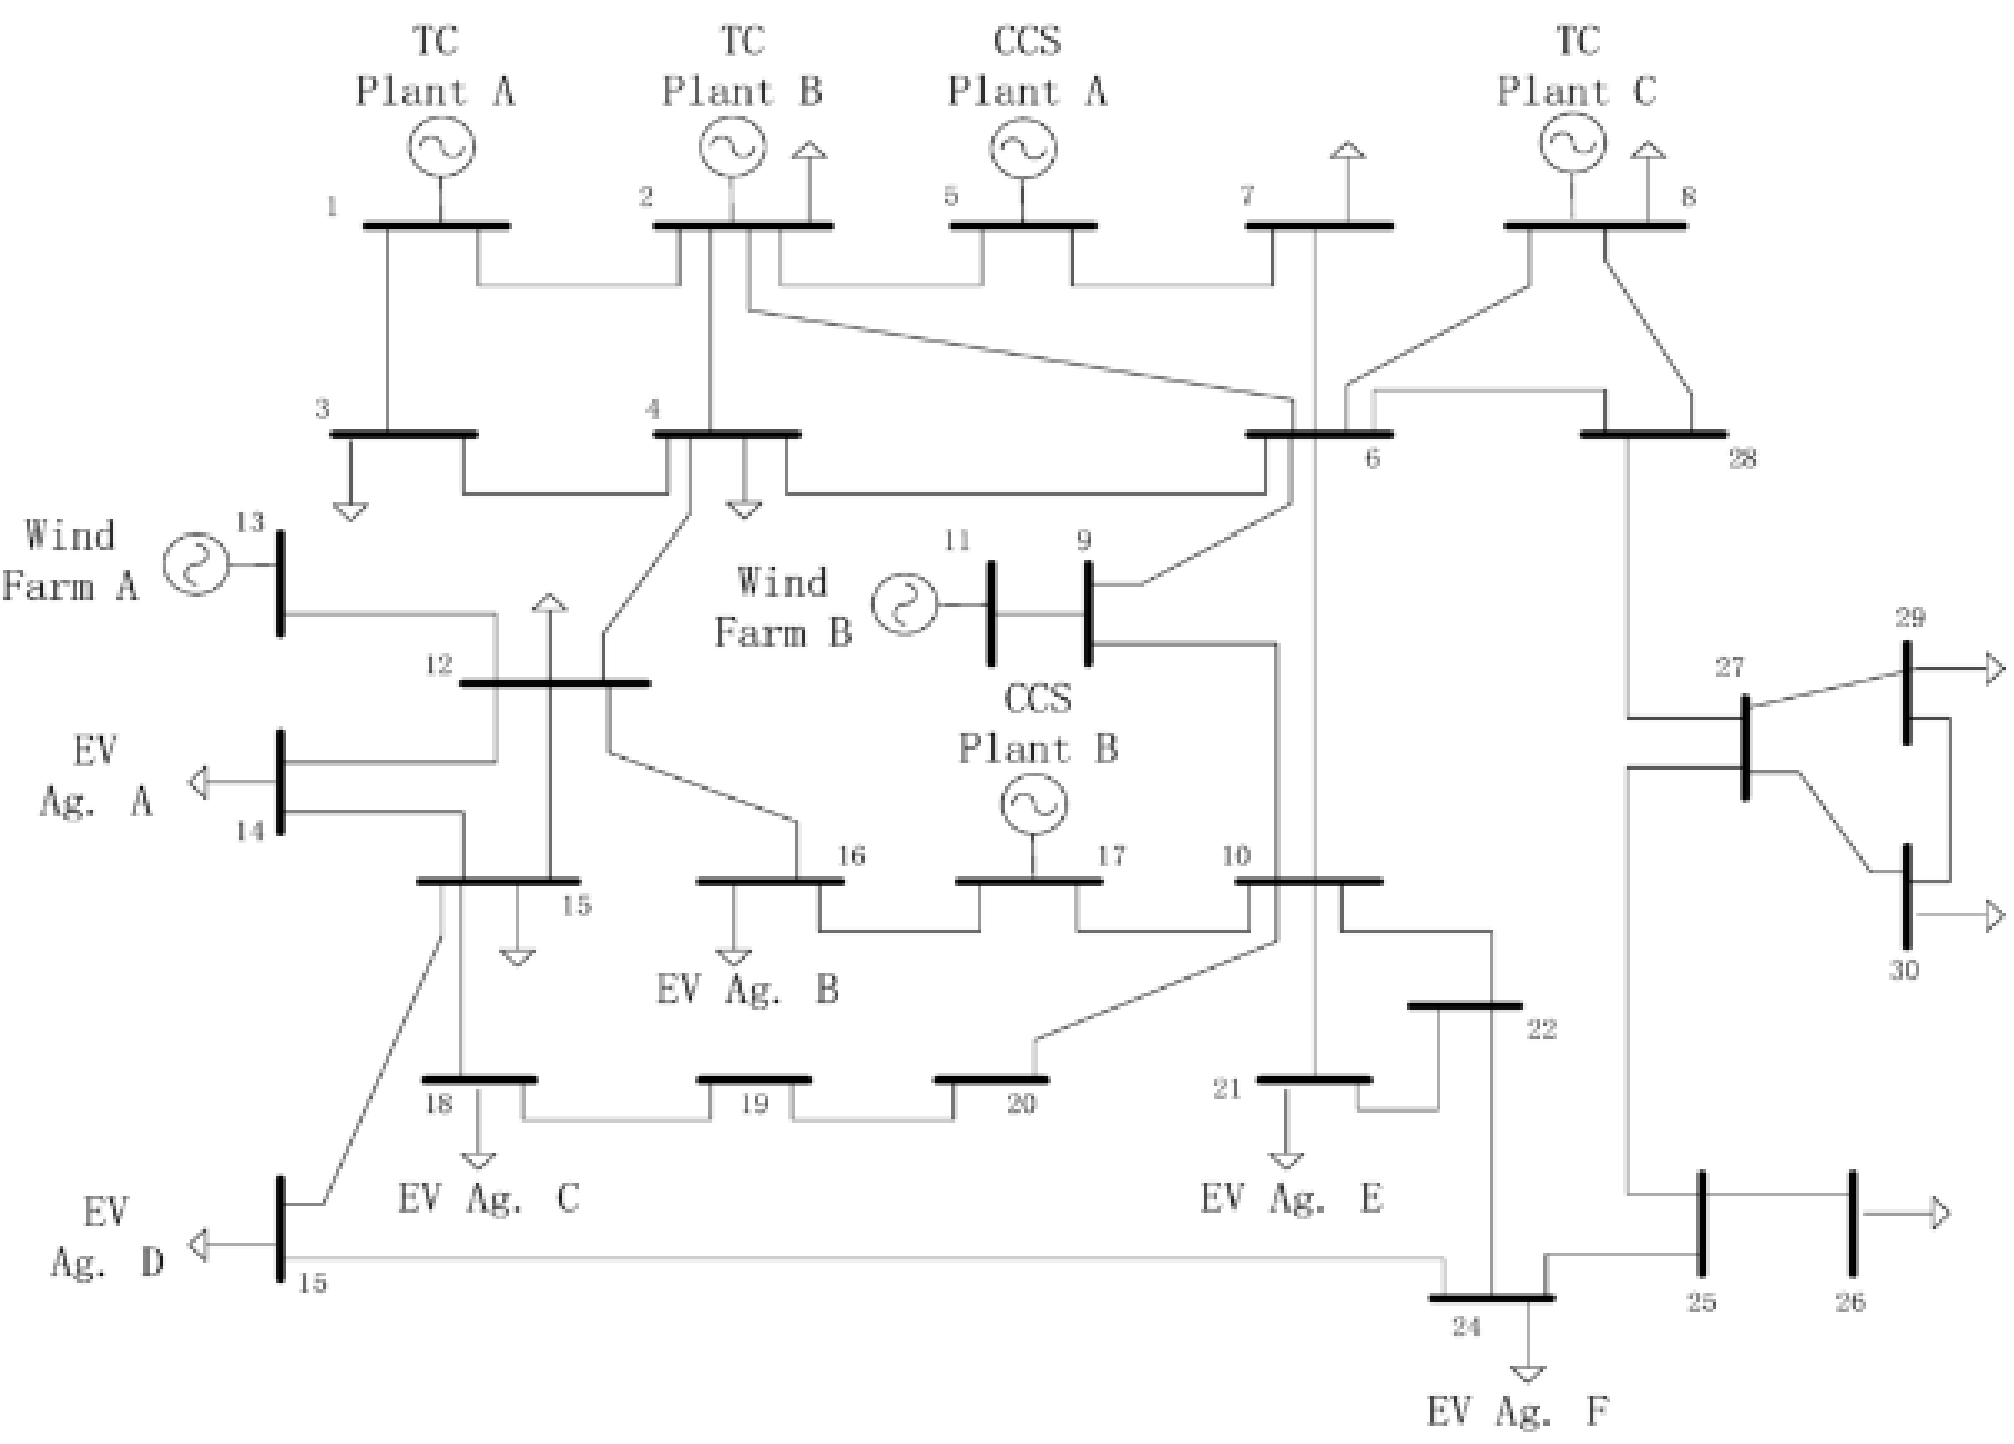
\includegraphics[width = \textwidth]{./img/figure45.png}
	\caption{Network at a works.}
\end{figure}
\subsection{Split distribution system - high integrity}
Non-essential loads (NE) are divided equally between two generators. Essential loads (E) have a cross-over connection capability either manual or automatic. This system ensures the integrity of the electrical system in case of generator failure.
\begin{figure}[H]
	\centering
	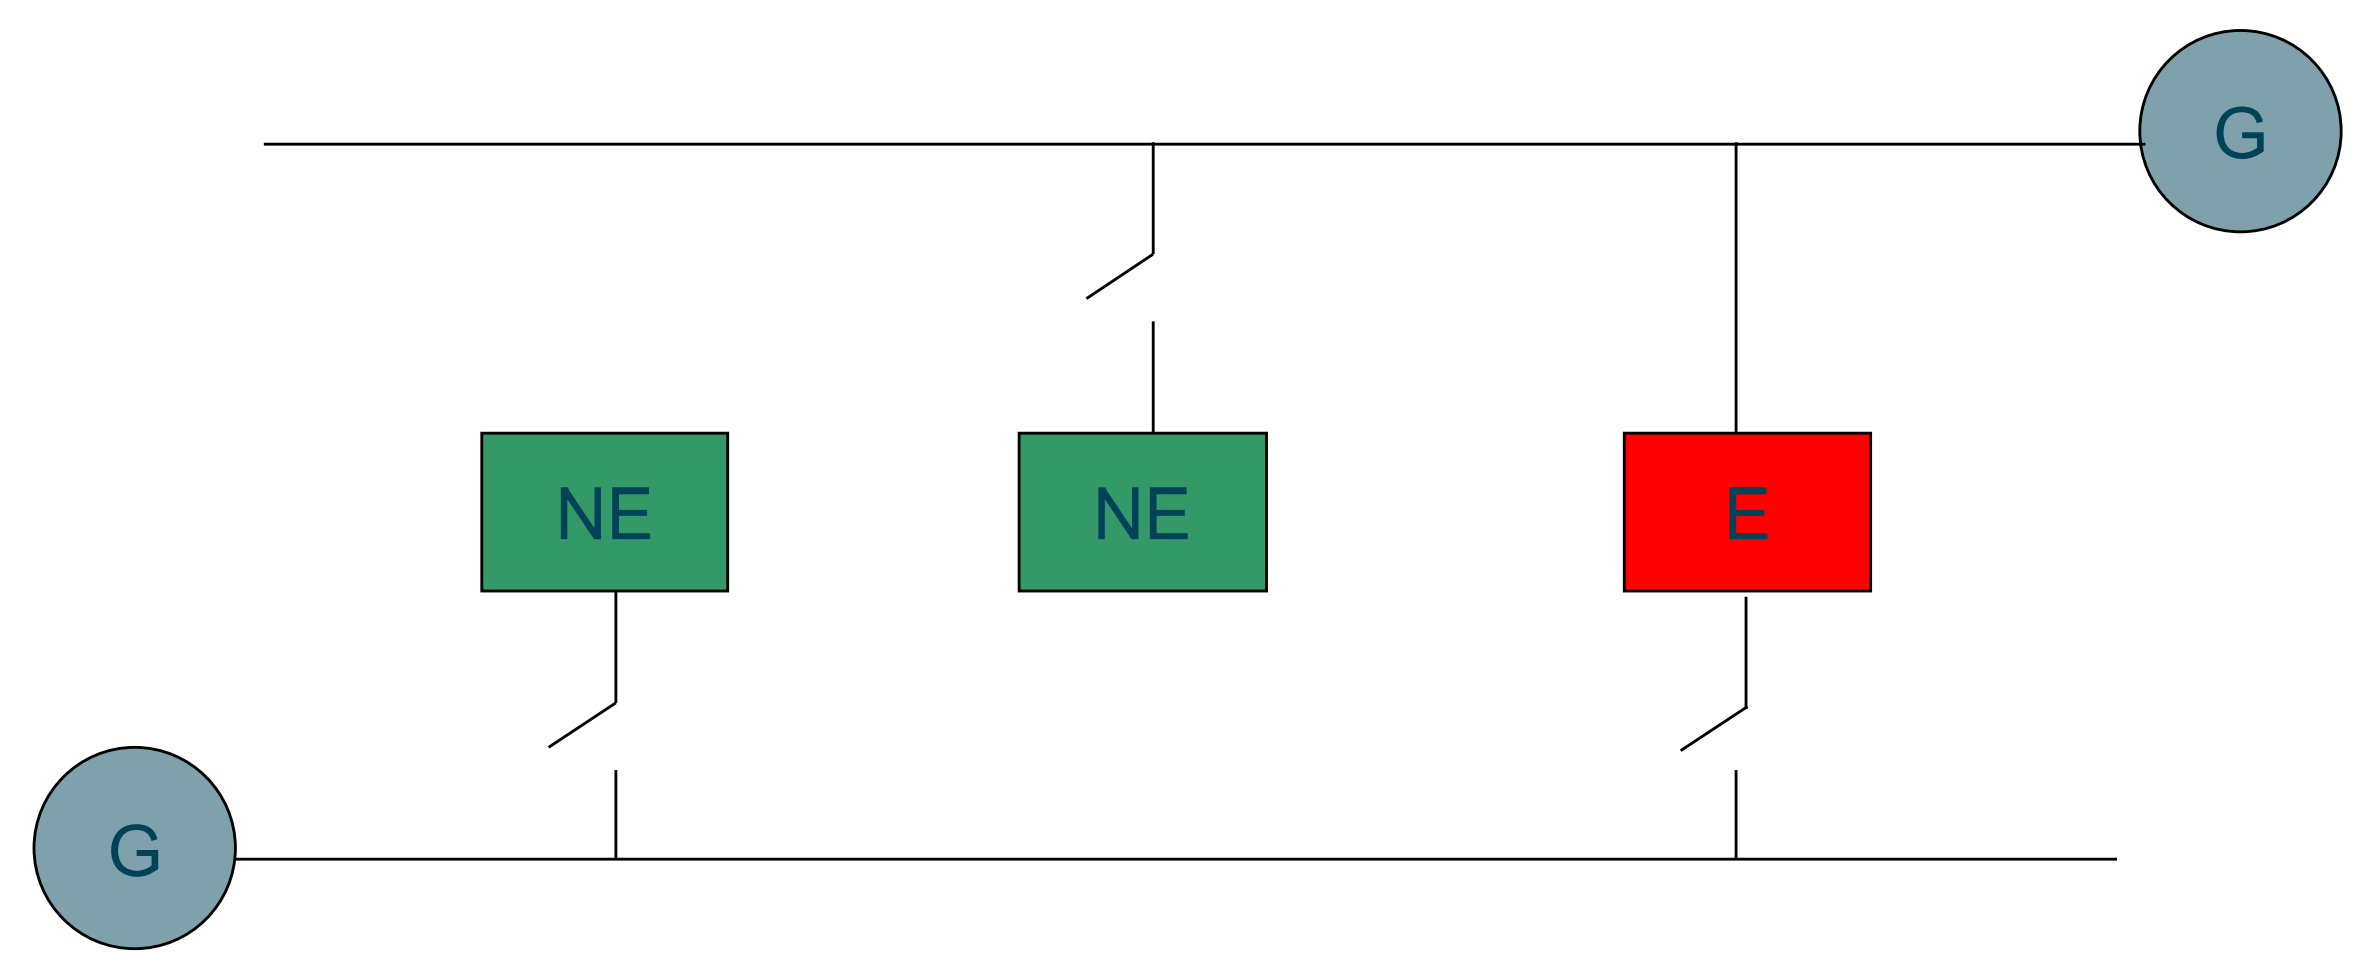
\includegraphics[width = \textwidth]{./img/figure46.png}
	\caption{Split distribution system - high integrity.}
\end{figure}
\subsection{Tree distribution}
Electrical power is generated (generators can be used in parallel) by the main generators to supply loads distibuted around the vessel. A small emergency generator is used as back-up to supply the emergency switchboard, which is usually supplied by the main board. 
\begin{figure}[H]
	\centering
	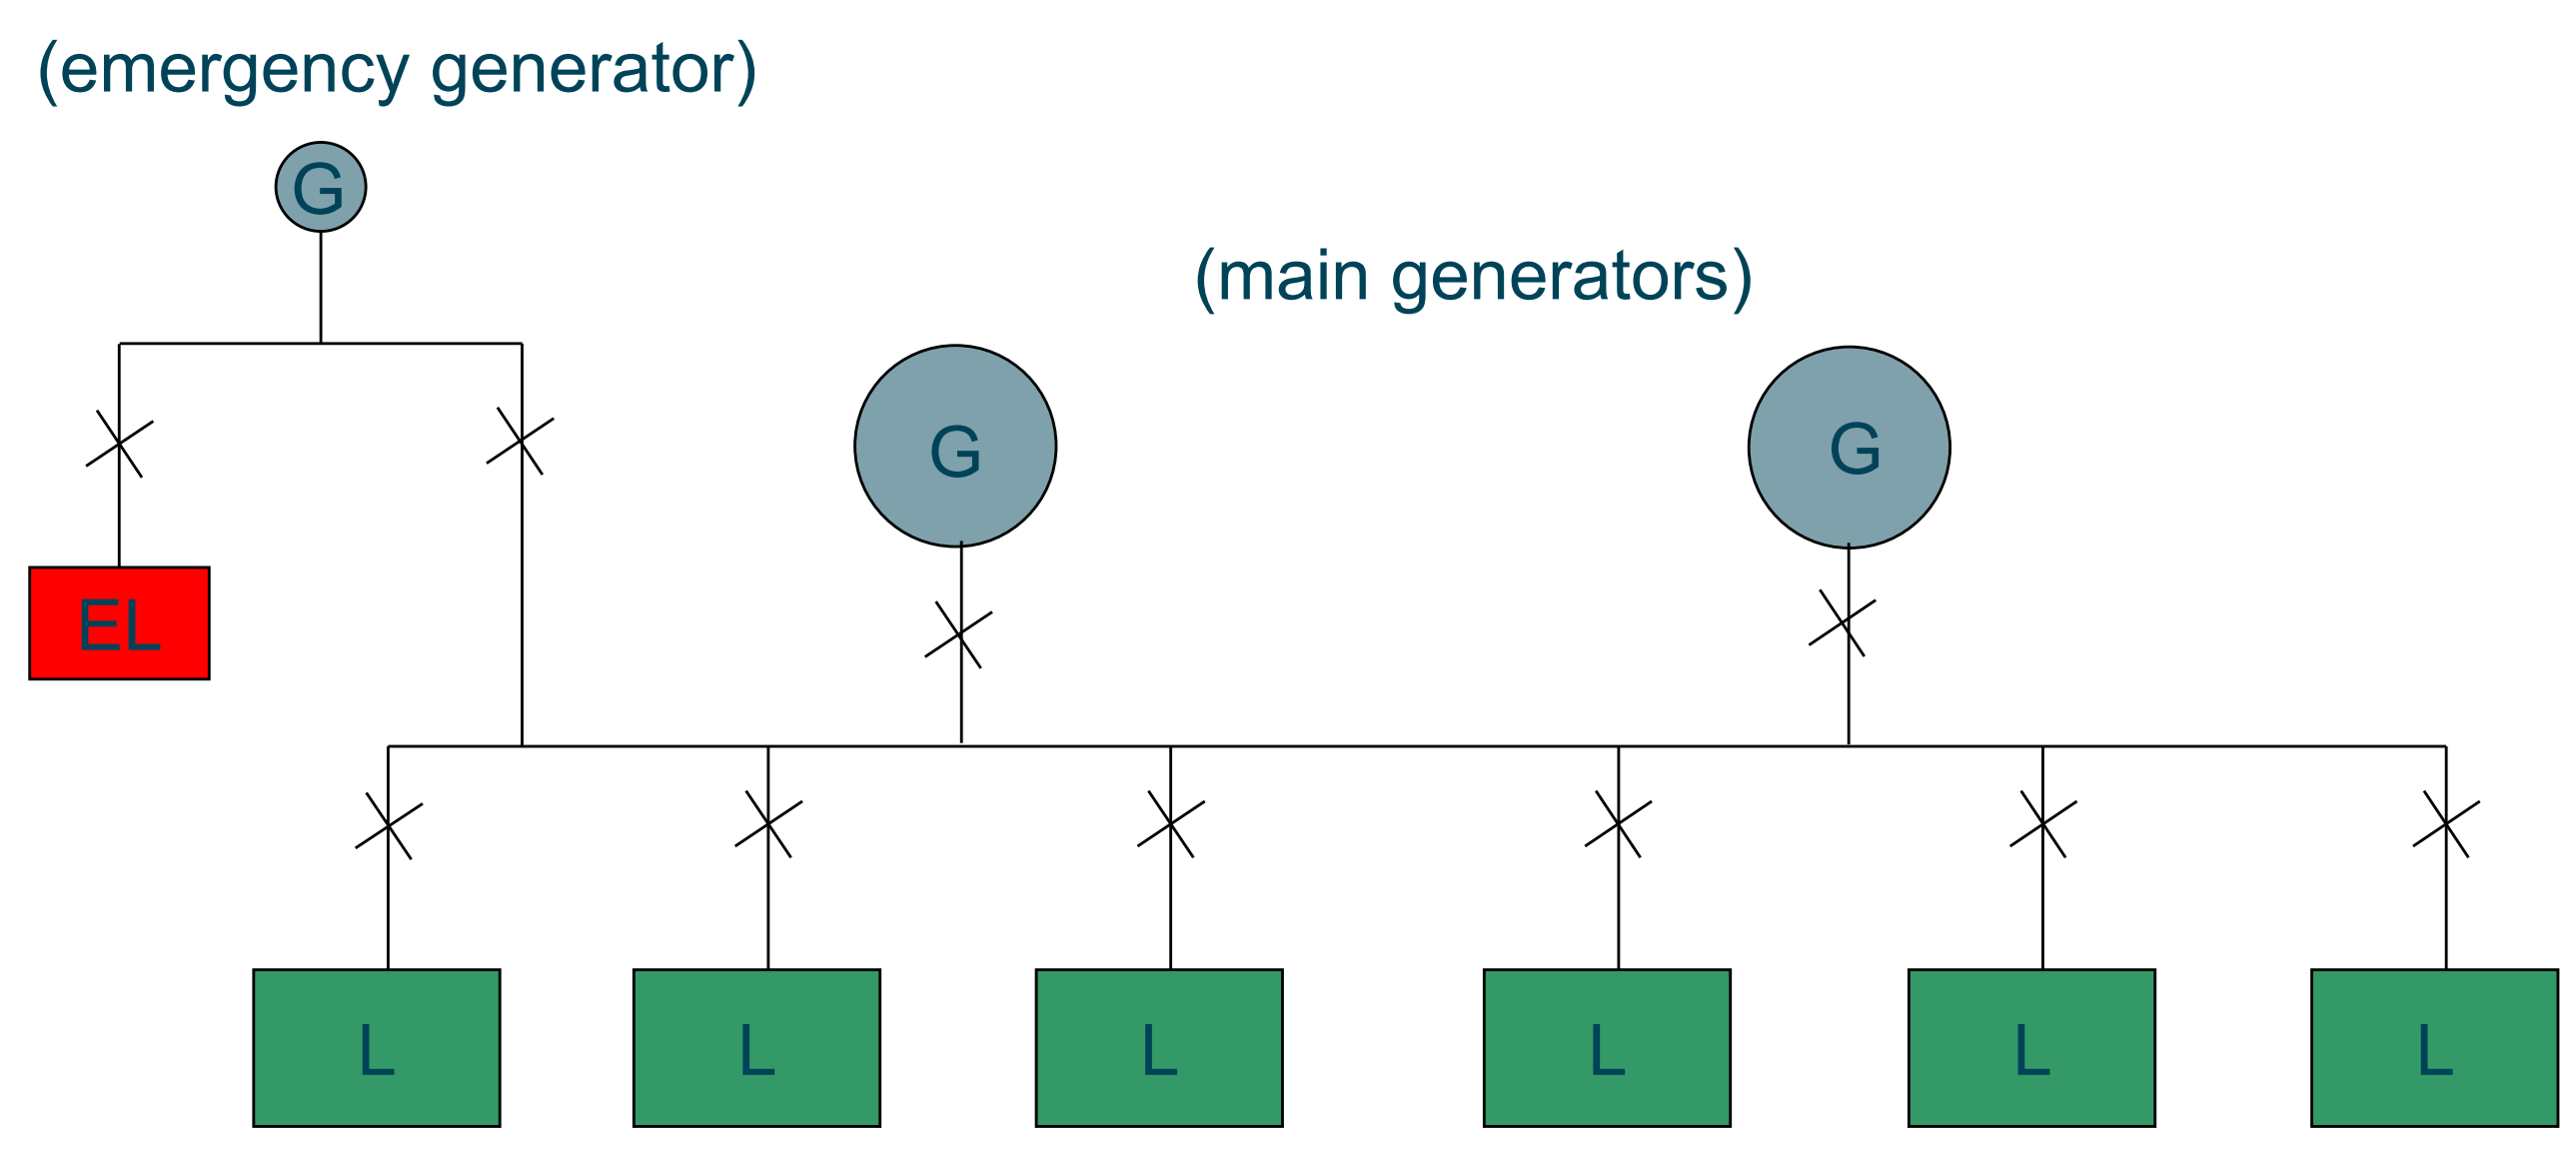
\includegraphics[width = \textwidth]{./img/figure47.png}
	\caption{Tree distribution.}
\end{figure}
\subsection{Ring networks - grids}
\begin{figure}[H]
	\centering
	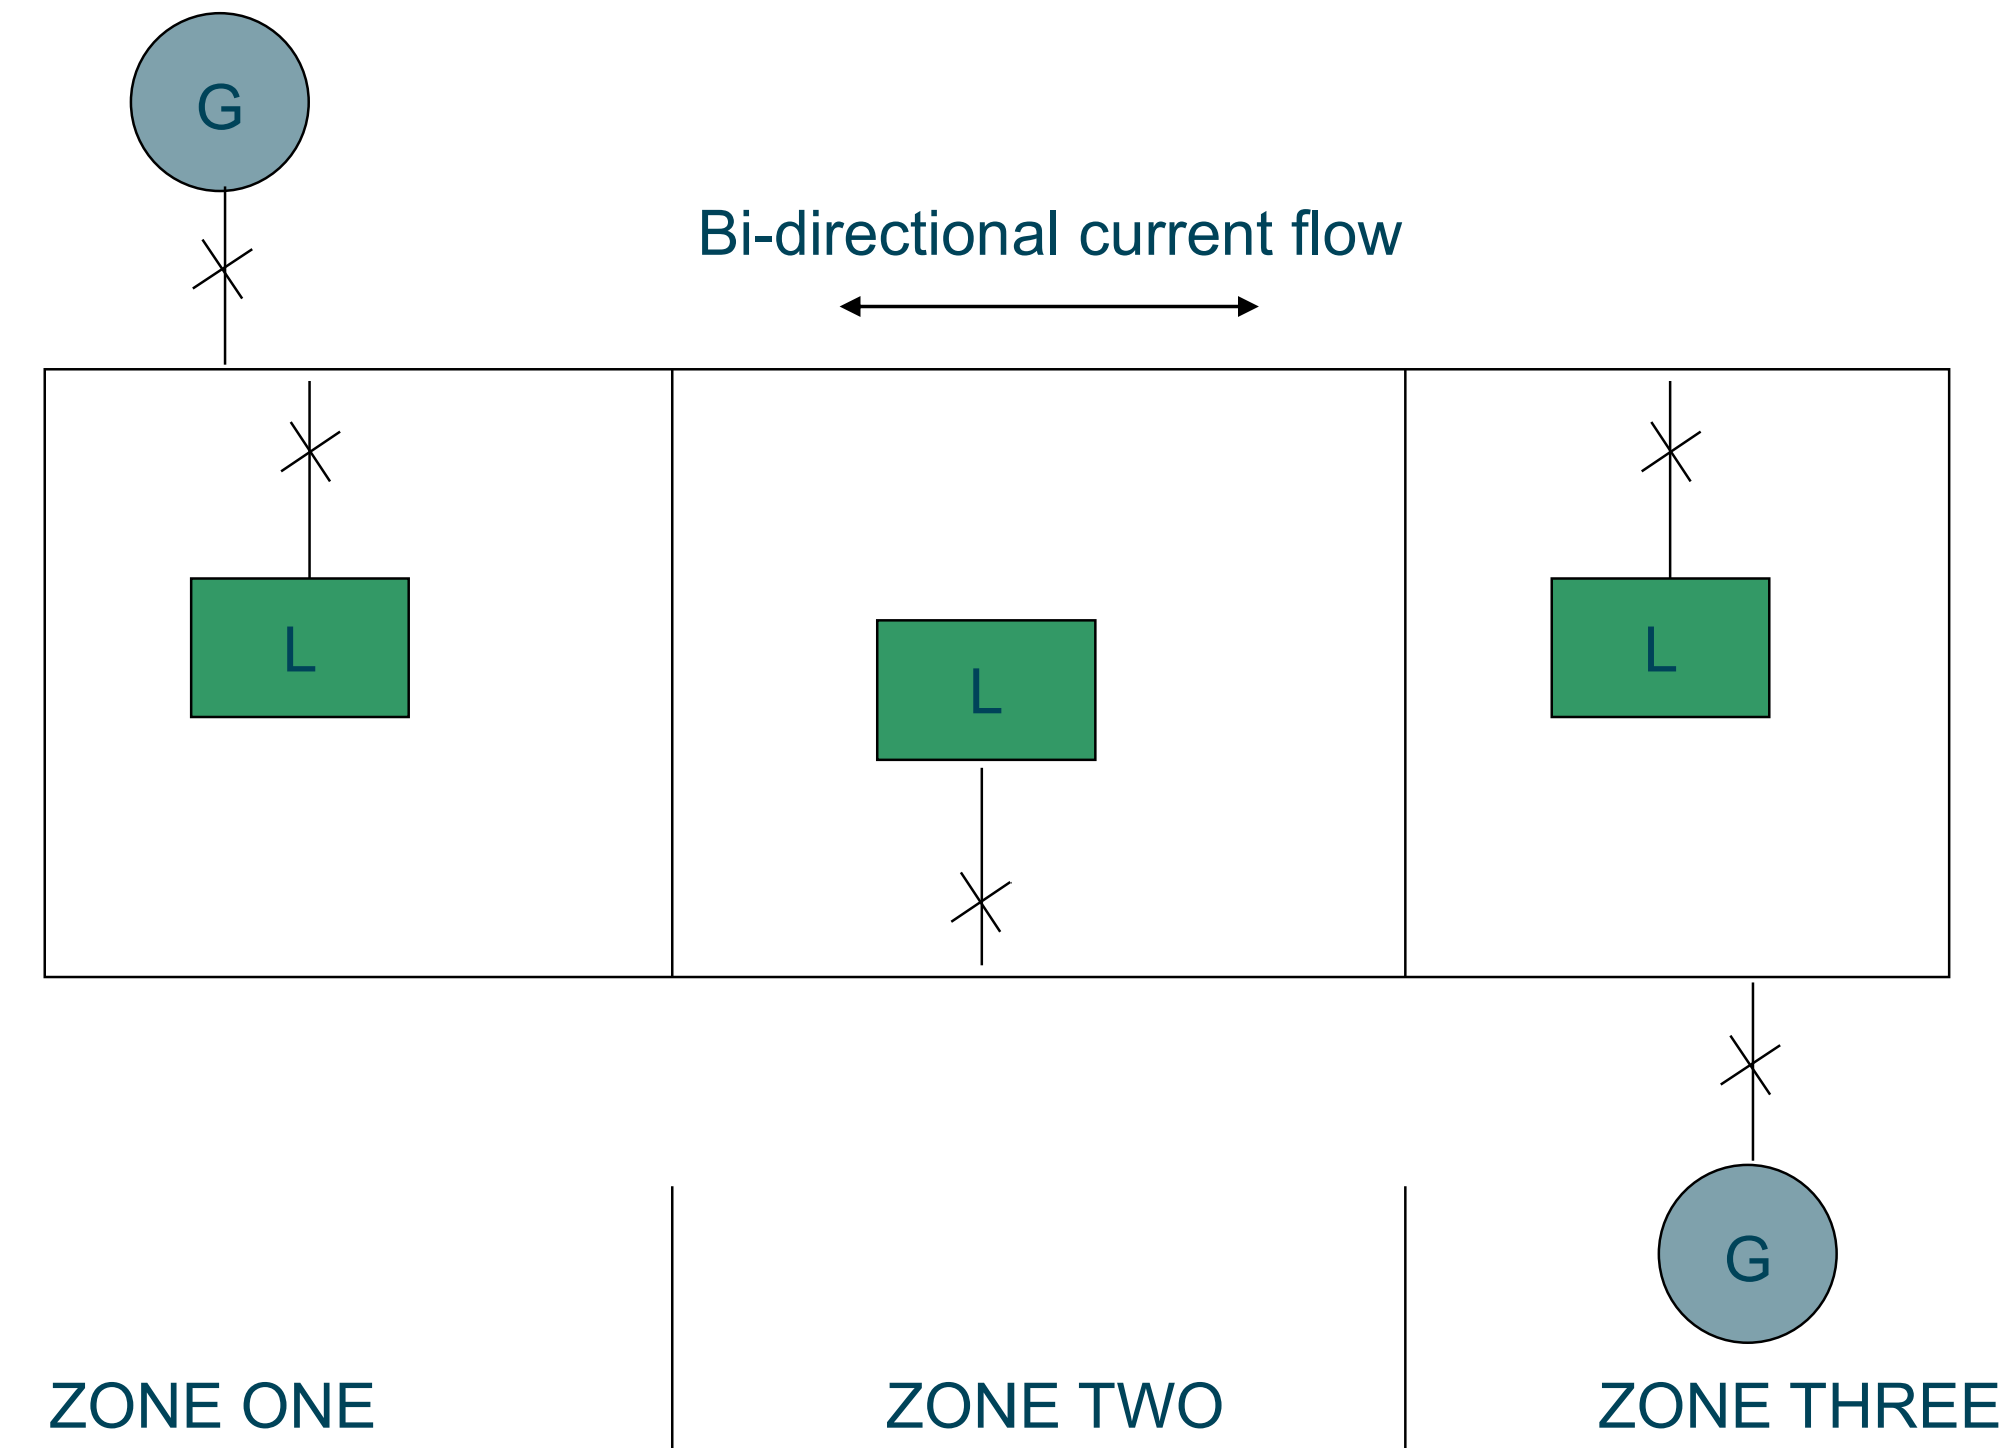
\includegraphics[width = \textwidth]{./img/figure48.png}
	\caption{Ring networks - grids.}
\end{figure}
\subsection{Network analysis}
It is essential to be able to analyse the performance of power systems whatever their design both during normal operating conditions and under fault (short-circuit) conditions. The analysis in normal steady-state operation is called a \textbf{power-flow study (load-flow study)} and it involves determing the voltages, current and real and reactive power flows in system under given load conditions. Earlier in the course, we examined the impact of an induction motor start. However, that was a single network and relatively straight forward. For more complex system, matrix methods are best used.

Today most power-flow studies are done by computer. The purpose of power flow studies is to plan ahead to be able to account for various hypothetical situations and understand steady-state, transient and faulted conditions. For instance, what if a transmission line within the power system properly supplying loads must be taken offline for maintenance. Can the remaining lines in the system handle the required loads without exceeding their rated parameters? For instance, what happens if a switchboard in a ship becomes faulty and need to be isolated or what happens when new equipment is fitted to an existing network?
\subsection{Techniques for power-flow studies}
A power-flow study (load-flow study) is an analysis of the voltages, currents and power flows in a power system and we will consider steady-state conditions. In such a study, we make an assumption:
\begin{enumerate}
	\item Either a \textbf{voltage} at a bus or the \textbf{power} being supplied to a bus for each bus in the power system
	\item We then determine the magnitude and phase angles of the bus voltages, line currents, etc. that would result from the assumed combination of voltages and power flows
	\item We use iterative methods of analysis to resolve
\end{enumerate}
\subsection{Power flow calculations}
The simplest way to perform power-flow calculations is by iteration. 
\begin{enumerate}
	\item Create a bus admittance matrix $Y_{bus}$ for the power system.
	\begin{itemize}
		\item \begin{gather}
			Y = \frac{1}{Z} = \left(G + jB\right)
		\end{gather}
		$G$ is conductance, $B$ is called susceptance and may be positive or negative. Note that: 
		\begin{gather}
			G = \frac{1}{R}, \quad B \neq \frac{1}{X}
		\end{gather}
	\end{itemize}
	\item Make an initial estimate for the voltages at each bus in the system (ideally something that is reasonable)
	\item Update the voltage estimate for each bus (one at a time), based on the estimates for the voltages and power flows at every other bus and the values of the bus admittance matrix (the voltage at a given bus depends on the voltages at all of the other buses in the system so even the updated voltage will not be correct but it will usually be closer to the answer than the original estimate). - An iterative method
	\item Repeat this process to make the voltages at each bus approaching the correct answers closer and closer\dots
\end{enumerate}
There are three types of defined bus:
\begin{itemize}
	\item Load bus
	\item Generator bus
	\item Slack bus
\end{itemize}
The process involves defining these buses and then sticking with that definition.
\subsection{Basic techniques for power-flow studies}
The equations used to update the estimates differ for different types of buses. Each bus in a power system can be classified to one of three types.
\begin{enumerate}
	\item \textbf{\underline{Load bus}} (PQ bus) - a bus at which the real and reactive power are specified, and for which the bus voltage will be calculated. \textbf{Real and reactive powers supplied to a power system are defined to be positive}, while the \textbf{powers consumed from the system are defined to be negative. All busses having no generators are load busses}
	\item \textbf{\underline{Generator bus}} (PV bus) - a bus at which the magnitude of the voltage is kept constant by adjusting the field current of a synchronous generator on the bus (\textbf{remember} - increasing the field current of the generator increases both the reactive power supplied by the generator and the terminal voltage of the system). We assume that the field current is adjusted to maintain a constant voltage $V_T$. We also know that increasing the prime mover's governor set points increases the power that the generator supplies to the power system and the frequency. Therefore, we can \textit{specify} the magnitude of the bus voltage and real power supplied
	\item \textbf{\underline{Slack bus}} (swing bus) - a \underline{special generator bus} serving as the reference bus for the power system. Its voltage is assumed to be fixed in both magnitude and phase (for instance, $1\angle\SI{0}{\degree}\, \si{pu}$). The real and reactive powers are uncontrolled: the bus supplies whatever real or reactive power is necessary to make the power flows in the system balance. 
\end{enumerate}
\subsection{Approach to analysis}
The most common approach to power-flow analysis is based on the bus admittance matrix $Y_{bus}$. However, this matrix is slightly different from the system previously since the internal impedances of generators and loads connected to the system are not included in the $Y_{bus}$. Instead, they are accounted for as specified real and reactive powers input and output from the buses.
\begin{figure}[H]
	\centering
	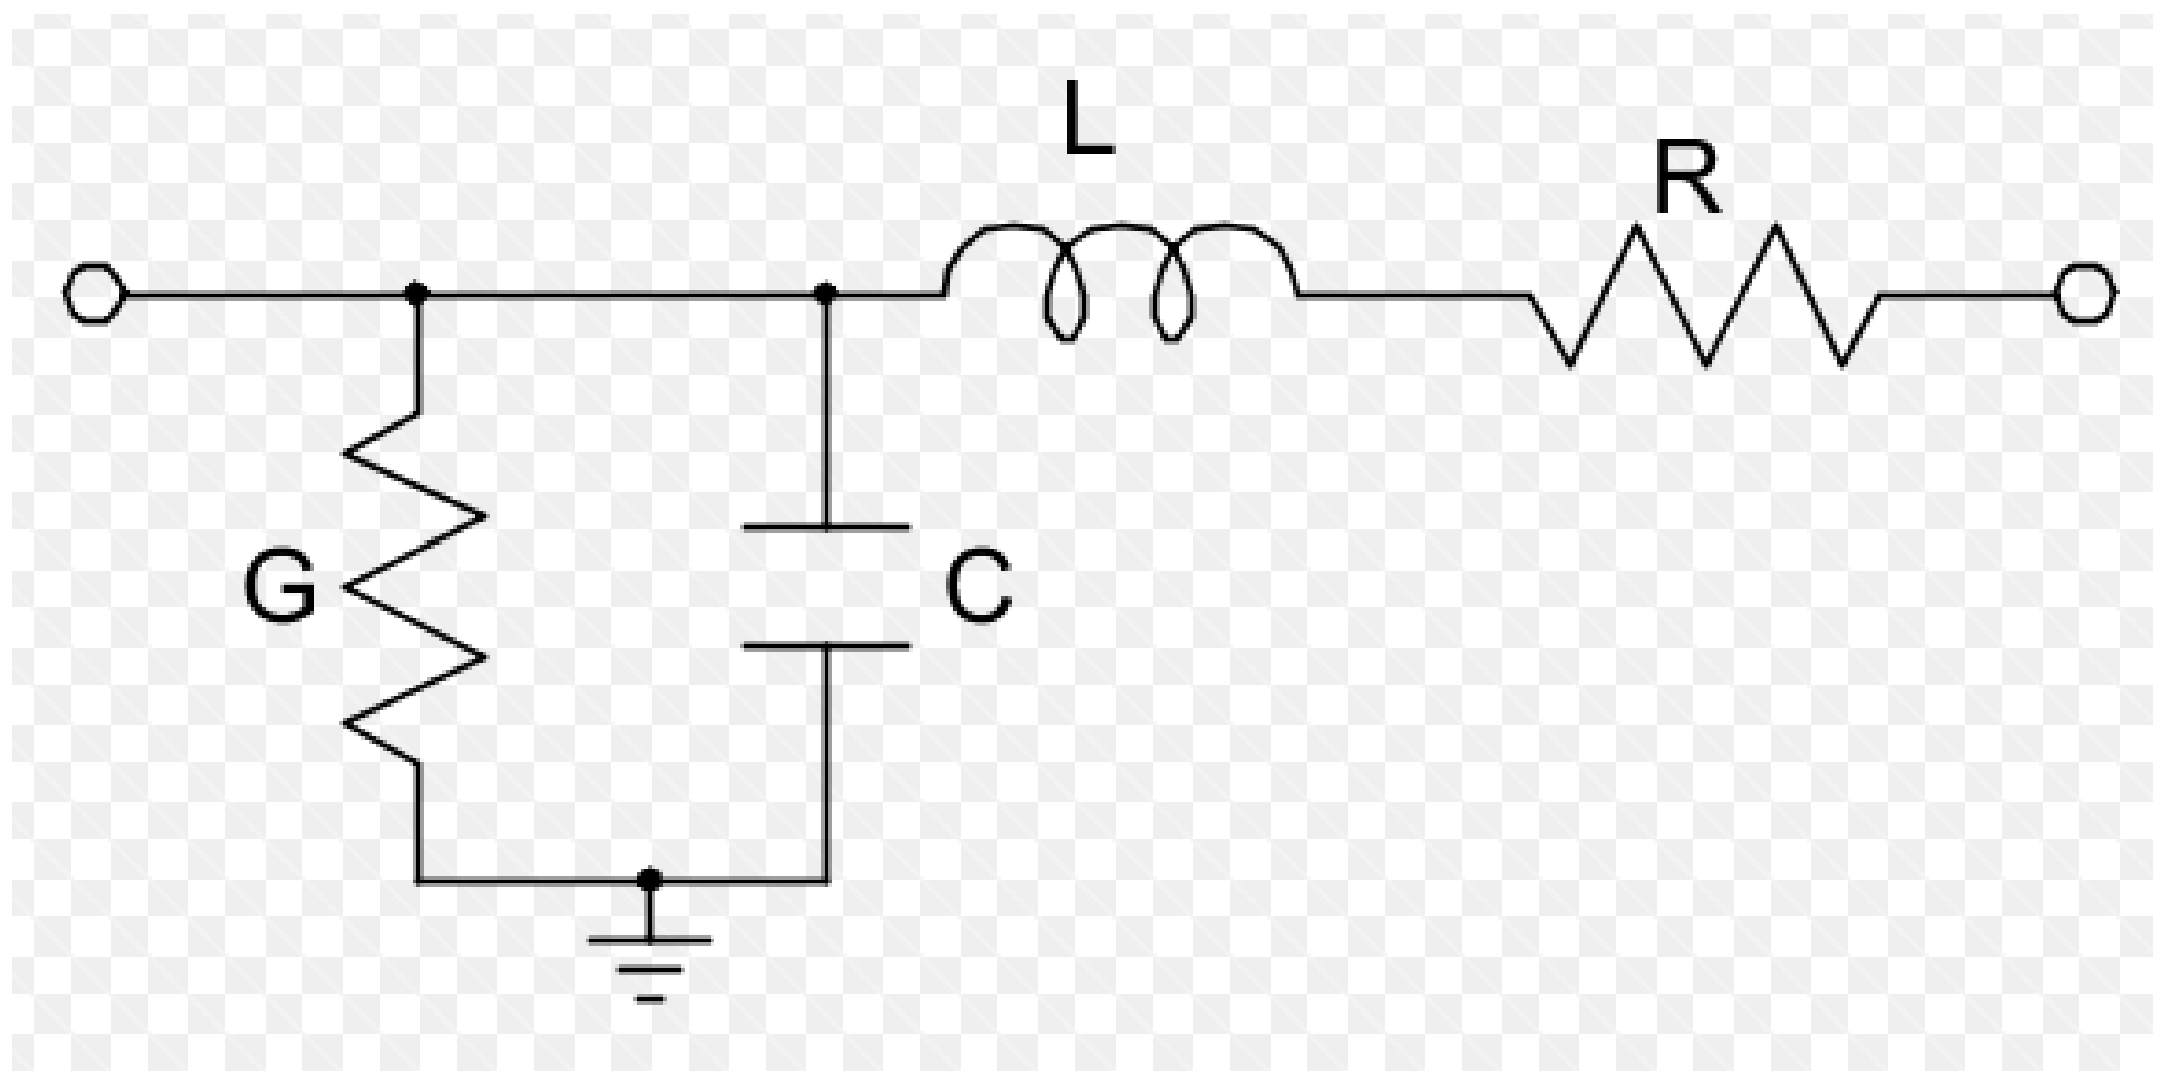
\includegraphics[width = 0.5\textwidth]{./img/figure49.png}
	\caption{Transmission line: only L and R are used in the $Y_{bus}$.}
\end{figure}
\subsection{Constructing $Y_{bus}$ for power-flow analysis}
Example 1: A simple power system has 4 busses, 5 transmission lines, 1 generator and 3 loads.
\begin{table}[H]
	\centering
	\begin{tabular}{@{}lll@{}}
		\toprule
		\textbf{line no.} & \textbf{Bus to bus} & \textbf{Series $Y$ (pu)}\\
		\midrule
		1 & 1-2 & $0.5882 - j2.3529$\\
		2 & 2-3 & $0.3846 - j1.9231$\\
		3 & 2-4 & $0.5882 - j2.3529$\\
		4 & 3-4 & $1.1765 - j4.7059$\\
		5 & 4-1 & $1.1765 - j4.7059$\\
		\bottomrule
	\end{tabular}
	\caption{Example 1 series per unit admittances.}
\end{table}
\begin{table}[H]
	\centering
	\begin{tabular}{@{}ll@{}}
		\toprule
		\multicolumn{2}{l}{\textbf{Table of busses}}\\
		\midrule
		Bus 1 & Slack bus\\
		Bus 2 & Load bus\\
		Bus 2 & Load bus\\		
		Bus 2 & Load bus\\
		\bottomrule
	\end{tabular}
	\caption{Example 1 table of busses.}
\end{table}
\begin{figure}[H]
	\centering
	\includegraphics[width = 0.7\textwidth]{./img/figure50.png}
	\caption{Transmission line: only L and R are used in the $Y_{bus}$.}
\end{figure}
The shunt admittances of the transmission lines are ignored. In this case, the $Y_{ii}$ terms of the bus admittance matrix can be constructed by summing the admittances of all transmission lines connected to each bus, and the $Y_{ij}\, (i \neq j)$ terms are just the negative of the line admittances stretching between busses $i$ and $j$. Therefore, for instance, the term $Y_{11}$ will be the sum of the admittances of all transmission lines connected to bus 1. which are the lines 1 and 5, so:
\begin{gather}
	Y_{11} = 1.7647 - j7.0588\, \si{pu}
\end{gather}
Note: if the shunt admittances of the transmission lines are not ignored, the self admittance $Y_{ii}$ at each bus would also include half of the shunt admittance of each transmission line connected to the bus.

The term $Y_{12}$ is defined as the negative of all the admittances stretching between bus 1 and bus 2, which will be the negative of the admittance of the transmission line 1, so:
\begin{gather}
	Y_{12} = -0.5882 + j2.3529
\end{gather}
The complete bus admittance matrix can be obtained by repeating these calculations for every term in the matrix.
\begin{gather}
	Y_{bus} = \begin{bmatrix}
		1.7647-j7.0588 & -0.5882 + j2.3529 & 0 & -1.1765 + j4.7059\\
		-0.5882 + j2.3529 & 1.5611-j6.5290 & -0.3746 + j1.9231 & -0.5882 + j2.3529\\
		0 & -0.3846+j1.9231 & 1.5611-j6.6290 & -1.1765 + j4.7059\\
		-1.1765+j4.7059 & -0.5882 + j2.3529 & -1.1765 + j4.7059 & 2.9412 - j11.7647
		\end{bmatrix}
\end{gather}
\subsection{Power-flow analysis equations}
The basic equation for power-flow analysis is derived fron the nodal analysis equations for the power system: 
\begin{gather}
	Y_{bus}V = I
\end{gather}
For the four-bus power system shown above, becomes:
\begin{gather}
	\begin{bmatrix}
		Y_{11} & Y_{12} & Y_{13} & Y_{14}\\
		Y_{21} & Y_{22} & Y_{23} & Y_{24}\\
		Y_{31} & Y_{32} & Y_{33} & Y_{34}\\
		Y_{41} & Y_{42} & Y_{43} & Y_{44}
	\end{bmatrix} \begin{bmatrix}
		V_1\\
		V_2\\
		V_3\\
		V_4
	\end{bmatrix}=\begin{bmatrix}
		I_1\\
		I_2\\
		I_3\\
		I_4
	\end{bmatrix}
\end{gather}
where $Y_{ij}$ are the elements of the bus admittance matrix, $V_i$ are the bus voltages, and $I_i$ are the currents injected at each node. FOr bus 2 in this system, this equation reduces to:
\begin{gather}
	Y_{21}V_1 + Y_{22}V_2 + Y_{23}V_3 + Y_{24}V_4 = I_2
\end{gather}
However, real loads are specified in terms of real and reactive powers, not as currents. The relationship between per-unit real and reactive power supplied to the system at a bus and the per-unit current injected into the system at that bus is:
\begin{gather}
	S = VI^* = P+jQ
\end{gather}
where $V$ is the per-unit voltage at the bus, $I^*$ is the complex conjugate of the per-unit current injected at the bus, $P$ and $Q$ are per-unit real and reactive powers. Therefore, for instance, the current injected at bus 2 can be found as:
\begin{gather}
	V_2 I^*_2 = P_2 + jQ_2 \rightarrow I^*_2 = \frac{P_2 + jQ_2}{V_2}
\end{gather}
Now the next steps are
\begin{enumerate}
	\item To switch $I^*_2$ and $V_2$ to use $I_2$ and $v_2^*$
	\item In doing so we have to change to $P$-$Q$ to keep sense
	\item Substitute $I$ for the relationships for $I = YZ$
\end{enumerate}
Implementing for $V_2$, yields\dots
\begin{gather}
	V_2 = \frac{1}{Y_{22}}\left[\frac{P_2-jQ_2}{V_2^*}-\left(Y_{21}V_1+Y_{23}V_3+Y_{24}V_4\right)\right]
\end{gather}
Similar equations can be created for each load bus in the power system.
\subsubsection{Gauss-Siedel iterative method}
Basic procedure:
\begin{enumerate}
	\item Calculate the bus admittance matrix $Y_{bus}$ including the admittances of all transmission lines, transformers, etc., between busses but exclides the admittances of the loads or generators themselves.
	\item Select a slack bus: one of the busses in the power system, whose voltage will arbitrarily be assumed as $1.0\angle\SI{0}{\degree}$.
	\item Select initial estimates for all bus voltages: usually, the voltage at every load bus is assumed as $1.0\angle\SI{0}{\degree}$ (flat start) lead to good covergence. Write voltage equations for every other bus in the system. The generic form is:
	\begin{gather}
		V_i = \frac{1}{Y_{ii}}\left(\frac{P_i-jQ_i}{V_i^*}-\sum^N_{k=1,\,k\neq i}T_{ik}V_k\right)
	\end{gather}
	\item Calculate an updated estimate of the voltage at each load bus in succession (except for the slack bus).
	\item Compare the differences between the old and new voltage estimates: if the differences are less than some specified tolerance for all busses, stop. Otherwise, repeat step 5.
	\item Confirm that the resulting solution is reasonable.
\end{enumerate}
\subsection{Example 2}
In a 2-bus power system, a generator attached to bus 1 and loads attached to bus 2. The series impedance of a single transmission line connecting them is $0.1 +j0.5\, \si{pu}$. The shunt admittance of the line may be negelected. Assume that bus 1 is the slack bus and that it has a voltage $V_1 = 1.0\angle\SI{0}{\degree}\,\si{pu}$. Real and reactive powers \underline{supplied} to the loads from the system at bus 2 are $P_2 = \SI{-0.3}{pu}$, $Q_2 = \SI{0.2}{pu}$. Determine voltages at each bus for the specified load conditions.
\begin{table}[H]
	\centering
	\begin{tabular}{@{}ll@{}}
		\toprule
		\multicolumn{2}{l}{\textbf{Table of busses}}\\
		\midrule
		Bus 1 & Slack bus\\
		Bus 2 & Load bus\\
		\bottomrule
	\end{tabular}
	\caption{Example 2 table of busses.}
\end{table}
\begin{figure}[H]
	\centering
	\includegraphics[height = 7cm]{img/figure51.png}
	\caption{Example 2 diagram.}
\end{figure}
\begin{enumerate}
	\item We start from calculating the bus admittance matrix $Y_{bus}$. The $Y_{ii}$ terms can be constructed by summing the admittances of all transmision lines connected to each bus, and the $Y_{ij}$ terms are the negative of the admittances of the line stretcing between busses $i$ and $j$. For instance, the term $Y_{11}$ is the sum of the admittances of all transmission lines connected to bus 1 (a single line in our case). The series admittance of line 1 is:
	\begin{gather}
		Y_{line1} = \frac{1}{Z_{line1}}= \frac{1}{0.1+j0.5} = 0.3846-j1.9231=Y_{11}
	\end{gather}
	Applying similar calculations to other terms, we complete the admittance matrix as:
	\begin{gather}
		Y_{bus} = \begin{bmatrix}
			0.3846-j1.9231 & -0.3846+j1.9231\\
			-0.3846+j1.9231 & 0.3846-j1.9231
		\end{bmatrix}
	\end{gather}
	\item Next, we select bus 1 as the slack bus since it is the only bus in the system connected to the generator. The voltage at bus 1 will be assumed $1.0\angle\SI{0}{\degree}$. 
	\item We select initial estimates for all bus voltages. Making a flat start, the initial voltage estimates at every bus are $1.0\angle\SI{0}{\degree}$. 
	\item Next, we write voltage equations for every other bus in the system. For bus 2:
	\begin{gather}
		V_2 = \frac{1}{Y_{22}}\left[ \frac{P_2-jQ_2}{V^*_{2,old}}-Y_{21}V_1 \right]
	\end{gather}
	Since the real and reactive powers \underline{suppled} at bus 2 are $P_2 = \SI{-0.3}{pu}$ and $Q_2 = \SI{0.2}{pu}$ and since $Y_s$ and $V_1$ are known, we may reduce the last equation:
	\begin{align}
		V_2 &= \frac{1}{0.3846 - j1.9231}\left[\frac{-0.3-j0.2}{V^*_{2,old}}-\left(\left(-0.3846+j1.9231\right)V_1\right)\right]\\
		&= \frac{1}{1.9612\angle\SI{-78.8}{\degree}}\left[\frac{0.3603\angle\SI{-146.3}{\degree}}{V^*_{2,old}}-\left(1.9612\angle\SI{101.3}{\degree}\right)\left(1\angle\SI{0}{\degree}\right)\right]
	\end{align}
	\item Next, we calculate an updated estimate of the voltages at each load bus in succession. In this problem we only need to calculate updated voltages for bus 2. since the voltage at the slack bus (bus 1) is assumed constant. We repeat this calculation until the voltage converges to a constant value. The initial estimate for the voltage is $V_{2,0} = 1\angle\SI{0}{\degree}$. The next estimate for the voltage is:
	\begin{align}
		V_{2,1} &= \frac{1}{1.9612\angle\SI{-78.8}{\degree}}\left[\frac{0.3603\angle\SI{-146.3}{\degree}}{V^*_{2,old}}-\left(1.9612\angle\SI{101.3}{\degree}\right)\left(1\angle\SI{0}{\degree}\right)\right]\\
		&= \frac{1}{1.9612\angle\SI{-78.8}{\degree}}\left[\frac{0.3603\angle\SI{-146.3}{\degree}}{1\angle\SI{0}{\degree}}-\left(1.9612\angle\SI{101.3}{\degree}\right)\left(1\angle\SI{0}{\degree}\right)\right]\\
		&= 1.0834\angle\SI{-9.0275}{\degree}
	\end{align}
	The new estimate for $V_2$ substituted back to the equation will produce the second estimate:
\end{enumerate}

%\newpage
%\bibliographystyle{unsrtnat}
%\bibliography{Refs.bib}
%\appendix
\chapter{Plots}
\begin{figure}[H]
    \centering
    \includegraphics[width = 0.8\textwidth]{img/Roll Type.pdf}
    \caption{RMSE results for Type-1 and Type-2 Configurations for Roll Output}
    \label{fig:roll_type}
\end{figure}
\begin{figure}[H]
    \centering
    \includegraphics[width = 0.8\textwidth]{img/Pitch Type.pdf}
    \caption{RMSE results for Type-1 and Type-2 Configurations for Pitch Output}
    \label{fig:pitch_type}
\end{figure}
\begin{figure}[H]
    \centering
    \includegraphics[width = 0.6\textwidth]{img/Yaw Type2.pdf}
    \caption{RMSE results for Type-1 and Type-2 Configurations for Yaw Output}
    \label{fig:yaw_type}
\end{figure}
\begin{figure}[H]
    \centering
    \includegraphics[width = 0.6\textwidth]{img/Thrust Type.pdf}
    \caption{RMSE results for Type-1 and Type-2 Configurations for Thrust Output}
    \label{fig:thrust_type}
\end{figure}
\begin{figure}[H]
    \centering
    \begin{minipage}[b]{0.45\textwidth}
        \includegraphics[height=5cm,keepaspectratio]{img/scenario1_pid_paths.eps}
        \caption{Scenario 1 Path taken using PID Drone Control}
        \label{fig:Paths1_pid}
    \end{minipage}
    \hfill
    \begin{minipage}[b]{0.45\textwidth}
        \includegraphics[height=5cm,keepaspectratio]{img/scenario1_fis_paths.eps}
        \caption{Scenario 1 Path taken using ANFIS Drone Control}
        \label{fig:Paths1_fis}
    \end{minipage}
\end{figure}
\begin{figure}[H]
    \centering
    \begin{minipage}[b]{0.45\textwidth}
        \includegraphics[height=5cm,keepaspectratio]{img/scenario2_pid_paths.eps}
        \caption{Scenario 2 Path taken using PID Drone Control}
        \label{fig:Paths2_pid}
    \end{minipage}
    \hfill
    \begin{minipage}[b]{0.45\textwidth}
        \includegraphics[height=5cm,keepaspectratio]{img/scenario2_fis_paths.eps}
        \caption{Scenario 2 Path taken using ANFIS Drone Control}
        \label{fig:Paths2_fis}
    \end{minipage}
\end{figure}
\begin{figure}[H]
    \centering
    \begin{minipage}[b]{0.45\textwidth}
        \includegraphics[height=5cm,keepaspectratio]{img/scenario3_pid_paths.eps}
        \caption{Scenario 3 Path taken using PID Drone Control}
        \label{fig:Paths3_pid}
    \end{minipage}
    \hfill
    \begin{minipage}[b]{0.45\textwidth}
        \includegraphics[height=5cm,keepaspectratio]{img/scenario3_fis_paths.eps}
        \caption{Scenario 3 Path taken using ANFIS Drone Control}
        \label{fig:Paths3_fis}
    \end{minipage}
\end{figure}
\begin{figure}[H]
    \centering
    \begin{minipage}[b]{0.45\textwidth}
        \includegraphics[height=5cm,keepaspectratio]{img/scenario4_pid_paths.eps}
        \caption{Scenario 4 Path taken using PID Drone Control}
        \label{fig:Paths4_pid}
    \end{minipage}
    \hfill
    \begin{minipage}[b]{0.45\textwidth}
        \includegraphics[height=5cm,keepaspectratio]{img/scenario4_fis_paths.eps}
        \caption{Scenario 4 Path taken using ANFIS Drone Control}
        \label{fig:Paths4_fis}
    \end{minipage}
\end{figure}
\begin{figure}[H]
    \centering
    \begin{minipage}[b]{0.45\textwidth}
        \includegraphics[height=5cm,keepaspectratio]{img/scenario5_pid_paths.eps}
        \caption{Scenario 5 Path taken using PID Drone Control}
        \label{fig:Paths5_pid}
    \end{minipage}
    \hfill
    \begin{minipage}[b]{0.45\textwidth}
        \includegraphics[height=5cm,keepaspectratio]{img/scenario5_fis_paths.eps}
        \caption{Scenario 5 Path taken using ANFIS Drone Control}
        \label{fig:Paths5_fis}
    \end{minipage}
\end{figure}

\end{document}